%------------------------------------------------------------------------------
% Exemplo de documento para auxiliar a padronização das monografias da 
% Faculdade de Economia - UFF
%------------------------------------------------------------------------------

\documentclass[12pt, openright, chapter=TITLE]{economia} %---------------------
% Estão disponíveis opções de impressão como frente e verso, papel A4, outras
% linguagens e ets...
%------------------------------------------------------------------------------ 

\usepackage{tikz}
\usepackage{amsmath}
\usepackage{longtable}
\usepackage{lscape}
%\usepackage{pdflscape}
\usepackage{threeparttable}
\usepackage{scalefnt}
\usepackage{amsfonts} 
\usepackage{helvet}
\renewcommand{\familydefault}{\sfdefault}
\usepackage{footnote}
\makesavenoteenv{tabular}
\makesavenoteenv{table}
%------------------------------------------------------------------------------
% INFORMAÇÕES E DADOS PARA A CAPA
%------------------------------------------------------------------------------

\titulo{Aplicações de Técnicas de Análise de Sentimentos às Atas do Comitê de Política Monetária: comparação dos períodos de 2003 à 2018}
\autor{Gustavo de Oliveira Vital}
\data{2019} 
\orientador{Prof. Dr. Jes\'us Alexei Luizar Obregon}
%\coorientador{Prof. Dr$^{a}$. Danielle Carusi Machado}

%------------------------------------------------------------------------------
%	FOLHA DE ROSTO E PREAMBULO
%------------------------------------------------------------------------------

\preambulo{Monografia apresentada ao curso de Bacharelado em Ciências Econômicas da Universidade Federal Fluminense como requisito parcial para conclusão do curso.}

%------------------------------------------------------------------------------
% INÍCIO DO DOCUMENTO
%------------------------------------------------------------------------------

\makeindex

\begin{document}

\imprimircapa 						
\imprimirfolhaderosto*	  					

\begin{folhadeaprovacao}

   	\pre
   
   	\vfill
   	Trabalho aprovado em XX de XXXXXXX de XXXX\\
   	\banca
   	\assinatura{\textbf{\imprimirorientador}\space Orientador \\ \uff} 
   	\assinatura{\textbf{Prof. Dr$^a$. } \\ \uff} % Escrever o nome do professor
   	\assinatura{\textbf{Prof. Dr. Emmanoel de Oliveira Boff} \\ \uff} % Se for outra instituição, escrever o nome
   	%\assinatura{\textbf{Professor} \\ Convidado 3}
   	%\assinatura{\textbf{Professor} \\ Convidado 4}
   	\vfill
	  
\end{folhadeaprovacao}	
\clearpage

\begin{agradecimentos}

\noindent
Agradeço a todas as pessoas que me apoiaram, sabendo que o fizeram ou não.\\

\noindent
Em especial, agradeço aos meus pais, Cesar e Katia por sempre terem me incentivado, apoiado, e por todas as oportunidades que me deram, proporcionando que eu pudesse estudar em uma universidade pública, gratuita e de qualidade. Agradeço também a todos aqueles que me acompanharam e acompanham desde o meu primeiro período na faculdade. Agradeço ao Programa de Educação Tutorial que, por mais de uma vez, me serviu como base para continuar na faculdade -- em especial aos dois tutores que tive nesse projeto: Renaut Michel e Lérida Povoleri, que infelizmente nos deixou neste ano de 2019. \\  

\noindent
Não poderia deixar de agradecer, além disso, à professora Danielle Carusi, que sempre me ajudou e aconselhou quando eu precisava, bem como pela oportunidade que me deu em contribuir para a Revista Econômica. Por fim, agradeço ao meu orientador, professor Jesús Alexei, por todo incentivo e ajuda que me deu, esperando sempre o melhor de mim e estando sempre presente para qualquer dúvida -- antes mesmo de ser meu orientador.

\end{agradecimentos}


% ------------------------------------------------------------------
% RESUMO E ABSTRACT
%
% Para iniciarmos um ambiente, seja de resumo, abstract ou outro 
% qualquer, devemos começar pelo \begin. Onde eu escrevo nesse 
% arquivo, já me encontro dentro de um ``ambiente de resumo''.
%
% Aqui, apresentarei o resumo e mais um outro comando de exemplo: o 
% \lipsum. A principal função do \lipsum é gerar textos aleatórios -
% textos dummys. Assim, por mais que no presente documento - 
% no arquivo .TeX - os \lipsum[3-5] ou \lipsum[2-4] apareçam, no 
% .pdf esses só aparecerão como textos aleatórios.
% ------------------------------------------------------------------

%\setlength{\absparsep}{18pt} % ajusta o espaçamento dos parágrafos do resumo
\begin{resumo}
Este estudo apresenta uma comparação das expressões do Comitê de Política Monetária, levando em consideração as publicações das atas disponíveis após cada reunião, para o período de 2003 à 2018 -- isto é, do período de gestão de Meirelles ao período de gestão Goldfajn. A estrutura metodológica e analítica deste trabalho apresenta as técnicas de coleta e mineração de dados; a divergência de Kullback-Liebler; índices de sentimentos; e modelos de vetores auto-regressivos, bem como a função de resposta ao impulso. Os resultados deste trabalho indicam que efetivamente a forma de expressão da política monetária é relacionada com o período a ser analisado, sendo demonstrado que, de fato, a as distribuições de termos e palavras diferem de acordo com o cenário político brasileiro (PT-PMDB), bem como índices de sentimentos podem ser considerados em modelos macroeconômicos para predizer fenômenos econômicos.

\textbf{Palavras-chave}: Analise de sentimentos; Mineração de texto; COPOM; Kullback-Liebler.
\end{resumo}

% ------------------------------------------------------------------
% No caso do abstract, faremos a mesma coisa. Só adicionaremos a 
% opção abstract como o argumento do comando.
%-------------------------------------------------------------------

\begin{resumo}[ABSTRACT] % ESCREVER EM LETRAS MAIÚSCULAS
	
This study compares the expressions of the Monetary Policy Committee, taking into account the publications of the minutes available after each meeting, from 2003 to 2018 - that is, from the Meirelles management period to the Goldfajn management period. The methodological and analytical structure of this paper presents the techniques of data collection and mining; the Kullback-Liebler divergence; indices of feelings; and autoregressive vector models, as well as the impulse response function. The results of this work indicate that the form of monetary policy expression is effectively related to the period to be analyzed, showing that, in fact, the distributions of terms and words differ according to the Brazilian political scenario (PT-PMDB), as well as sentiment indices can be considered in macroeconomic models to predict economic phenomena.

\textbf{Keywords}: Sentiment analysis; Text mining; COPOM; Kullback-Liebler. 	
\end{resumo}






\figuras

\tabelas

\sumario


% -----------------------------------------------------------------------------
% ELEMENTOS TEXTUAIS
% -----------------------------------------------------------------------------

\textual




\chapter{Introdução}

% o que é analise de sentimento
% breve histórico da análise de sentimento
% como é feita?
% por que ela é feita? Destacar ṕotencialidades da metodologia

% Quais são os objetivos gerais? Ex: ajudar a compreender tal fenômeno
% Quais são os objetivos específicos? Ou seja, o que exatamente se pretende com o trabalho? São objetivos-meio para alcançar o objetivo geral. Ex: comprovar que a evasão aumentou nos últimos anos para contribuir na elucidação do fenômeno da evasão. Este ponto tem a ver com as conclusões. Se as conclusões alcançam esses objetivos, o trabalho foi bem sucedido.

% Estrutura do trabalho
% Quais são os capítulos?
% O que será discutido em cada capítulo?
% O que se pretende alcançar com cada capítulo?

É sabido que a tomada de decisões em diversas áreas econômicas têm, por vezes, como referência boletins e resoluções de bancos centrais. Como todo documento textual, atas e boletins contém informações objetivas e subjetivas quantificáveis possibilitando uma relação com a atividade econômica; política econômica ou mesmo uma análise específica em relação à análise de conjuntura de um certo período - no que se refere as informações objetivas. É possível, através de modelagem econométrica, mapear posições de agentes econômicos, bem como trazer expectativas dos respectivos comportamentos.

%É possível, desta forma, \textit{mapear} posições de agentes econômicos afim de modelar econometricamente para melhor entendermos as posições desses agentes, bem como suas expectativas.

Naturalmente, pelas características das informações dos agentes, é esperado que o mapeamento destes fenômenos econômicos não siga o mesmo padrão diante diferentes momentos conjunturais.  

Em geral, análise de sentimentos pode ser considerada uma técnica computacional de manipulação e análise de dados que consiste em extrair e classificar informações contidas em textos naturais. O objetivo é encontrar opiniões, expressões, e mensagens que um ou mais textos podem transmitir - dado um texto, classificá-lo como positivo ou negativo, por meio de identificações de padrões e características desse texto.   

Ainda, é possível melhor entender a abordagem relativa a um texto dado um cenário econômico, social ou geo-político. Até então, pouco utilizada no âmbito econômico, essa técnica é comumente relacionada aos campos das ciências políticas e de marketing. Um dos principais motivos de não se trabalhar com análise de sentimentos em questões econômicas é não ser óbvio - a princípio - que textos podem ser analisados e classificados como dados quantitativos, o que é uma contradição frente ao aspecto de bancos centrais utilizarem ferramentas e técnicas estatísticas que permitem esse feito \cite{bholat2015text}.        

Um outro fator a ser discutido é a possibilidade de realização dessa técnica. Como se trata, majoritariamente, de uma técnica computacional e comumente é relacionado ao campo de \textit{big data}, seria inviável a utilização dessa sem uma adequada capacidade de processamento e armazenamento de dados, o que explica um crescimento recente no uso da análise de sentimentos - visto que cada vez mais computadores são capazes de processar e armazenar informações.  

A presente monografia visa estudar no contexto de análise de sentimentos as expressões das atas do Comitê de Política Monetária (COPOM) no período de 2003-2018, Lula-Temer. Dessa forma, a análise feita é referente aos três diferentes períodos de presidência do Banco Central: Henrique Meirelles; Alexandre Tombini; e Ilan Goldfajn. É verificada uma mudança nos padrões das distribuições relativas aos períodos das palavras que mais aparecem. Para a contestação das mudanças referentes as distribuições, utiliza-se a divergência de Kullback-Leibler (também conhecida como entropia relativa) \cite{kullback1951information}. %De forma geral, se a divergência de Kullback-Leibler for igual a zero, podemos esperar o mesmo comportamento entre as distribuições das palavras, enquanto uma entropia relativa igual a um indicaria que as distribuições das séries se comportariam de maneira diferente. É apresentado, além disto, os dicionários utilizados na análise de sentimentos deste trabalho, bem como suas metodologias de composição. 

O segundo capítulo deste trabalho contém essencialmente uma explicação mais aprofundada sobre análise de sentimentos e \textit{text mining}, evidenciando a importância dessas duas técnicas como parte fundamental e específica do campo da ciência de dados, bem como suas aplicabilidades. Ainda, é feita uma revisão dos tipos e características das formas de realizar essa técnica, seja ela com o uso - ou não - de dicionários de \textit{stopwords}, ou algoritmos de \textit{machine learning}. Neste capítulo, discute-se, também, a abordagem da análise de sentimentos por bancos centrais e pesquisas com base em trabalhos empíricos já realizados.

O terceiro caítulo se inicia com uma explicação das principais técnicas utilizadas nesta monografia. São elas: o \textit{web scraping} empregado, bem como o funcionamento de um algoritmo de \textit{web scraping}; tratamento dos dados e a metodologia utilizada para o tratamento dos mesmos; o dicionário de \textit{stopwords} utilizado e o porquê de utiliza-lo; e a metodologia utilizada em relação a análise de sentimentos em si. Além disso, é explicado o porquê da utilização da linguagem R na utilização desse trabalho, bem como os pacotes dessa linguagem contidos no projeto. %É explicado, também, o porquê das atas analisadas estarem em inglês (minutes). 

O quarto capítulo, por sua vez, apresenta os resultados empíricos do trabalho. Entre esses podemos citar comparações entre as frequências de palavras; a ocorrência geral das palavras corrigidas pelos tamanhos das atas; comparações das principais palavras frentes aos momentos de conjunturas analisados; e a análise de sentimentos nas atas do COPOM.

Finalizamos com o quinto capítulo, evidenciando as considerações finais do trabalho e as conclusões referentes ao que foi feito.

%Por fim, estão conditas as seções de apêndice da monografia. Nos anexos são apresentadas as principais tabelas referentes aos dicionários (\textit{stopwords}, léxico); tabelas de frequência das palavras utilizadas por períodos; tabelas de correções de palavras, assim como a metodologia utilizada para cada correção em particular; tabelas das 400 palavras que mais aparecem numa análise geral (sem distinção de termos econômicos); gráficos de distribuição e histogramas das palavras de cunho econômico que mais aparecem; resultados dos testes estatísticos; e referências aos códigos utilizados nesta monografia por meio de um repositório online. 
\chapter{Revisão da literatura}

\section{Preliminar}

A crescente pesquisa por análise de sentimentos e \textit{text mining} tende a corroborar, de forma geral, para um melhor entendimento do que acontece no cenário mundial econômico, por meio de \textit{proxys} que por muitas vezes não podem ser captadas senão de forma computacional. Compreender melhor a demanda por alguma coisa torna-se mais fácil, no quesito em que é possível automatizar resoluções de problemas econômicos e não econômicos. Como um próprio exemplo disso, podemos nos fazer valer da própria busca pelo termo \textit{sentiment analysis}. A Figura \ref{fig:google} apresenta a evolução da busca pelo termo \textit{sentiment analysis}, desde 2004 até o mês de outubro de 2019 -- A busca foi realizada no dia primeiro de novembro de 2019, com os seguintes parâmetros: 1 - termo de pesquisa: sentiment analysis; 2 - foi aplicado um período de busca de 2004 até o mês de outubro de 2019; Para todo o mundo, todas as categorias, e pesquisa na web. No volume de busca, 100 representa o máximo volume como referência. 

\begin{figure}[!h]
    \centering
    \caption{Evolução da busca pelo termo \textit{sentiment analysis}, de janeiro de 2004 até outubro de 2019}
    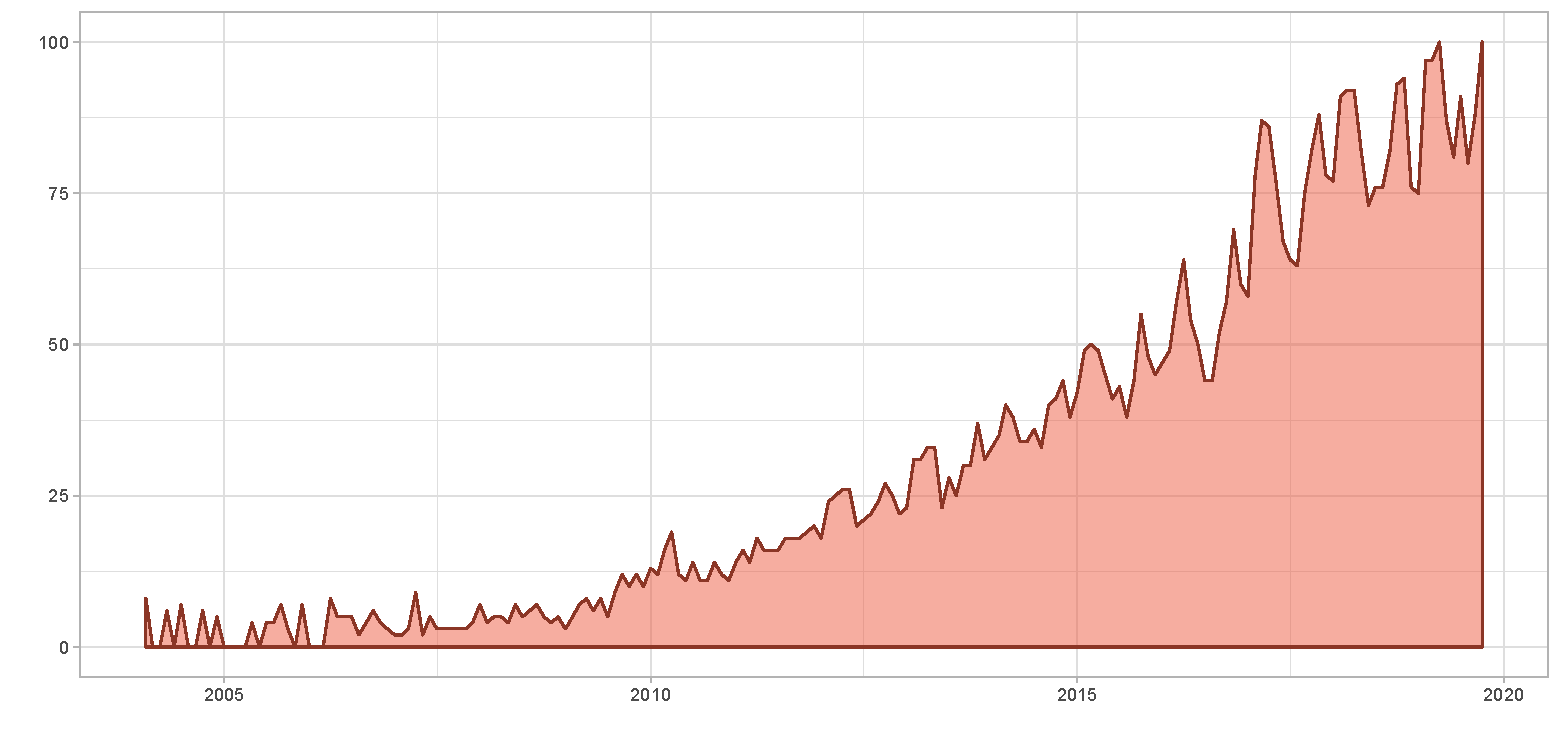
\includegraphics[width=\textwidth]{capitulos/figures/google.pdf}
    \fonte{Google trends. Elaboração própria.}
    \label{fig:google}
\end{figure}

Ainda, acrescenta-se, mesmo que atualmente o volume de buscas por esse termo seja quase insignificante para o Brasil (cerca de 4), países como a Índia ou a China apresentam volumes de buscas muito maiores: 81 e 22, respectivamente. A Índia é o pais que mais busca por esse termo. Tal qual, pode ser uma relação direta na crescente potencialidade tecnológica e de pesquisa deste país. 

\section{Mineração Textual}

Processamento de linguagem natural, conhecido também como \textit{Text Minning}, é um conjunto de procedimentos que utiliza ferramentas computacionais e técnicas estatísticas que permitem quantificar textos. Este processo de quantificação permite intuir algum significado textual -- indubitavelmente, por meio de um computador a análise e organização dos significados textuais podem ser feitas de formam muito mais precisa e automática do que de forma manual. O \textit{text mining}, ainda, possibilita a extração de \textit{significados} de textos, que podem ser difíceis de se identificar quando analisados sem o auxílio de um computador -- nos permite detectar padrões pouco prováveis ante às perspectivas humanas.

Mesmo quando muito usada em outros campos científicos, como ciências políticas e marketing, a técnica de \textit{text minning} ainda é pouco utilizada nas ciências econômicas como enuncia \citeonline{bholat2015text}

\begin{citacao}``Primeiro, pode não ser óbvio que o texto possa ser descrito e analisado como dados quantitativos. Como resultado, provavelmente existe uma falta de familiaridade nos bancos centrais com as ferramentas e técnicas estatísticas que tornam isso possível. Segundo, mesmo que os banqueiros centrais tenham ouvido falar em mineração de texto, eles já têm acesso a outros dados quantitativos prontamente disponíveis. A oportunidade e outros tipos de custos de transformar textos em dados quantitativos e aprender novas ferramentas e técnicas para analisar esses dados podem ser vistos como superando os benefícios esperados.
\footnote{First, it may not be obvious that text can be described and analysed as quantitative data. As a result, there is probably a lack of familiarity in central banks with the tools and statistical techniques that make this possible. Second, even if central bankers have heard of text mining, they already have access to other readily available quantitative data. The opportunity and other types of costs from transforming texts into quantitative data, and learning new tools and techniques to analyse these data, may be viewed as outweighing the expected benefits. \cite[p.1]{bholat2015text}}'' \cite[p.1]{bholat2015text}
\end{citacao}

Assim, a inserção do \textit{text mining} no campo da ciência econômica se apresenta de forma tardia, devido a obstáculos computacionais e por vezes desconfiança por parte dos agentes econômicos acostumados com informações quantitativas tradicionais. Uma análise a partir destes pode, ainda mais, incluir aspectos não convencionais em modelos micro e macroeconômicos, como possíveis \textit{proxys} de conjuntura política, interesses populacionais ou mesmo opiniões públicas. É notável, então, que a utilização de técnicas de \textit{text mining} poderia ser utilizada de maneira extremamente proveitosa por, por exemplo, bancos centrais. Isso é, extrair informações de formas não usuais de fontes que permitam, de alguma forma, avaliar estabilidade monetária e financeira de maneira quantitativa. Ou seja, a partir de notícias, jornais, artigos científicos, relatos de inteligência de mercado, ou mesmo relatórios empresariais, afim de quantificar estes dados para uma melhor obtenção da situação conjuntural vigente. 

A análise de um documento, ou um conjunto de documentos (tecnicamente chamado de \textit{corpus}) se daria, por exemplo, a partir de boletins informacionais de órgãos de pesquisa (vide por exemplo uma carta de conjuntura do Ipea - Instituto de Pesquisa Econômica Aplicada) ou mesmo atas de instituições financeiras.

Mesmo que ainda não seja uma técnica usual de análise, bancos centrais já se fazem valer de benefícios do \textit{text mining} diariamente. Uma busca online por determinados termos econômicos, dependendo da forma como é feita, ou mesmo proteção contra \textit{cyber-attacks} ou busca por uma base de dados de citações, no âmbito acadêmico, são exemplos usuais da funcionalidade do \textit{text mining} \cite{bholat2015text}.

\section{Análise de Sentimentos}

Em um recente artigo publicado pelo Banco da Inglaterra, \citeonline{bholat2015text},  é relatado os interesses dos bancos centrais e como estes, por meio textuais, não são devidamente aproveitados. Um exemplo de aplicação em relação a estes volumes de dados é a própria pesquisa realizada na internet, em termos econômicos ou mesmo em relação ao volume de buscas. Ainda podemos citar a correlação entre Jobseeker’s Allowance (JSA) e a taxa oficial de desemprego no Reino Unido, como mostra \citeonline{mclaren2011using}:

\begin{citacao}``É notável que os 'empregos', que provavelmente foram pesquisados por quem está dentro e fora do emprego, não aumentaram muito durante a recessão. As pesquisas por "desempregados" aumentaram acentuadamente durante a recessão. O termo "JSA" (sigla para Subsídio de Desemprego) foi escolhido porque seus movimentos melhor se correlacionaram com os dos dados oficiais. Também é provável que seja usado por aqueles que pensam que podem em breve ficar desempregados e, portanto, buscam mais informações sobre benefícios de desemprego.\footnote{It is notable that ‘jobs’, which is likely to have been searched for by both those in and out of employment, did not increase much during the recession.  Searches for ‘unemployed’ rose markedly during the recession.  The term ‘JSA’ (acronym for Jobseeker’s Allowance) was chosen because its movementsbest correlated with those in the official data.  It is also a termlikely to be used by those who think they may soon become unemployed and so search for more information on unemployment benefit. \cite[p.136]{mclaren2011using}}'' \cite[p.136]{mclaren2011using}
\end{citacao}

Faz sentido uma busca na internet por ``emprego'' quando a pessoa está desempregada, bem como por ``auxílio desemprego'' (Jobseeker’s Allowance). No mesmo artigo, os autores vão além: é possível identificar, ainda, uma correlação entre ``inflação imobiliária'' e ``agentes imobiliários''. Assim, a partir de expressões como ``preços de casas''; ``comprar imóvel''; e ``vender imóvel'' é possível obter uma \textit{proxy} para a demanda por moradia:

\begin{citacao}``Para o mercado imobiliário, segue-se uma abordagem semelhante à adotada acima para o mercado de trabalho. Uma proporção significativa de pesquisas relacionadas a habitação é para sites de empresas específicas. No entanto, essas pesquisas variam ao longo do tempo, dependendo da popularidade de cada site. Portanto, uma ampla variedade de termos de pesquisa genérica é considerada (incluindo "preços de casas", "casa de compra", "casa de venda", "hipoteca" e "agentes imobiliários"). Os termos de pesquisa 'comprar casa' e 'vender casa' foram inicialmente considerados, pois capturariam a demanda e a oferta de casas.\footnote{For the housing market a similar approach is followed to thattaken above for the labour market.  A significant proportion ofhousing-related searches are for specific companies’ websites.However, these searches vary over time depending on thepopularity of each website.  So a wide range of more genericsearch terms are considered (including ‘house prices’, ‘buyhouse’, ‘sell house’, ‘mortgage’ and ‘estate agents’).  The searchterms ‘buy house’ and ‘sell house’ were initially considered,since they would capture the demand for and supply of houses. \cite[p.137]{mclaren2011using}}'' \cite[p.137]{mclaren2011using}
\end{citacao}

Em ambos os casos, os autores obtiveram exito em suas pesquisas, o artigo ``Using internet search data as economic indicators'' \cite[p.136]{mclaren2011using}, publicado também pelo Banco da Inglaterra, apresenta resultados econométricos significativos frente a regressões utilizando variáveis reais regredidas em variáveis obtidas por meio de volume de buscas online. Isso é, seja em relação à taxa de desemprego como em relação à inflação imobiliária, ambas as séries puderam ser explicadas por meio das séries dos volumes de pesquisa online -- Nos exemplos citados no texto, o mecanismo de busca utilizado foi o \textit{google trends}.

Outra maneira de se aproveitar algorítimos e volumes de buscas online é levar em consideração medidas de risco e incerteza no âmbito econômico e financeiro dado um determinado momento. Uma recente contribuição nessa direção foi apresentada por \citeonline{nyman2018news}: é proposta uma teoria sobre ``hipótese financeira emocional'', a qual sustenta que ``os indivíduos se convencem a assumir posições nos mercados financeiros, criando narrativas sobre os possíveis resultados de suas ações''\footnote{``individuals gain conviction to take positions in financial markets by creating narratives about the possible outcomes of their actions'' \cite{nyman2018news, bholat2015text}}. Os autores correlacionam emoções de ``exitação'' com ganhos financeiros e ``ansiedade'' com possíveis perdas. Essas narrativas, entretanto, não são compostas de simples textos, e sim de interações sociais entre agentes. As hipóteses foram testadas a partir de três textos fundamentais: the Bank’s daily market commentary (2000-2010), broker research reports (2010-2013) and the Reuters’ News Archive (1996-2014). A partir disto, os autores propõe um índice de medida de sentimento textual:

$$SI_t=\frac{N_e - N_a}{N_t}$$ 

\noindent
onde $N_e$ e $N_a$ representam o número de palavras correlacionadas com os estados de, respectivamente, excitação e ansiedade. $N_t$ denota o número total de palavras do documento. O sinal do índice nos fornece um indicativo do que acontece no mercado: sendo esse positivo é simbolizado crescimento financeiro; caso negativo, uma retração no mercado financeiro -- respectivamente \textit{bullish} e \textit{bearish}.
%caso positivo, há o chamado \textit{bullish}\footnote{No mercado financeiro, \textit{bullish} representa o ataque de um touro. Isso é, atacando de baixo para cima -- simbolizando o crescimento financeiro} - isso é, quando o mercado está em ascensão; caso contrário (sinal negativo), determina-se um momento de \textit{bearish}\footnote{No mercado financeiro, \textit{bearish} representa o ataque de um Urso. Isso é, atacando de cima para baixo -- simbolizando uma queda financeira}
O índice, então, é comparado com outros eventos históricos e outros indicadores financeiros \cite{bholat2015text}. 

Uma vez que a incerteza econômica é medida, esta poderia ser utilizada como uma variável explicativa em modelos de bancos centrais - essa torna-se, então, um possível indicador quanto às orientações de política monetária de bancos centrais.

A análise de sentimentos pode ser definida como o resultado de uma sequência hierarquizada de processos de ``classificação''. Por sua vez, a classificação é entendida como uma função, ou domínio, em um conjunto de entidades e imagens em um conjunto binário: positivo, negativo. Indo além, existem três principais níveis de classificação em análise de sentimento: documento, aspecto e sentença.

\begin{citacao}``
Em documentos o objetivo é classificar a opinião do documento como expressando um sentimento ou opinião positiva ou negativa. É considerado o documento em sua totalidade como uma unidade de informação (falando sobre um tópico). Com
relação às sentenças, o objetivo é classificar o sentimento expresso em cada sentença. O primeiro passo é identificar se a sentença é subjetiva ou objetiva. Se a sentença é subjetiva a análise determinará se a sentença expressa opiniões positivas ou negativas. Já em nível de aspecto, o alvo é classificar o sentimento com relação as aspectos específicos das entidades a partir da identificação das entidades e seus aspectos dada a possibilidade de existir diferentes opiniões sobre aspectos distintos da mesma entidade (como em: A qualidade da chamada do telefone não é boa, mas a bateria dura muito tempo). '' \cite[p.12]{costa2016ensaios}
\end{citacao}

Em geral, pode-se classificar algorítimos de análise de sentimentos de duas formas: baseados em \textit{machine learning}, sendo possível dividir esses algorítimos em forma de aprendizado supervisionado e aprendizado não supervisionado; a outra forma é trabalhar por meio de dicionários (\textit{léxicos}). Como exemplo, podemos citar o dicionário \texttt{qdap} contido no pacote de mesmo nome do R implementado por \citeonline{qdapdict} que pode determinar, segundo seus critérios de análise, se uma palavra pode ser classificada como positiva ou negativa.

Para exemplificarmos a utilização de um dicionário léxico, um trabalho recente de \citeonline{costa2016ensaios}, apresenta uma análise de sentimentos para as atas do Comitê de Política Monetária para o período de 2000 à 2016. No estudo, um \textit{corpus} é composto por 157 atas e analisado e, por meio deste, um índice é proposto, onde $I_t$ é o índice de sentimento:
\begin{align} \label{indicecosta}
    I_t = \frac{NP_t - NN_t}{N} \quad ,
\end{align}


\noindent
para cada ata divulgada em $t$, $NP_t$ é a quantidade de palavras ``positivas'', $NN_t$ a quantidade de palavras ``negativas'', e $N$ a quantidade de palavras na ata \cite[p.13]{costa2016ensaios}.

Os autores chegam a conclusão, finalmente, de uma correlação entre determinadas variáveis macroeconômicas (taxa de juros Selic, IPCA, IPCA Meta) e o índice para tomada de decisão da autoridade monetária. A correlação se apresenta de maneira mais forte no que diz respeito ao comportamento de longo prazo dessas variáveis. Em períodos de alta de inflação há uma diminuição do \textit{score} do índice de sentimentos, o que representa uma maior cautela na expectativa econômica representada pela maior quantidade de palavras ``negativas'' utilizadas nas atas divulgadas no período analisado. Comportamento análago ocorre quando se compara o \textit{score} do índice com a taxa de juros Selic.

\section{Aplicações Econométricas}

Formuladores de políticas econômicas (\textit{policy makers}) e aqueles que participam do mercado confiam amplamente em uma variedade de modelos que incorporam o que é chamado de informação branda. Ao contrário de informações complexas, que incluem variáveis objetivas e diretamente quantificáveis (como produção e taxa de desemprego), informações brandas influem medidas subjetivas relativas a atitudes em relação às condições econômicas atuais e futuras. Há, assim, uma ampla variedade de variáveis flexíveis disponíveis, mas sem dúvida as mais amplamente levadas em consideração  são as medidas relativas às confianças de mercado e sentimento do consumidor \cite{shapiro2018measuring}.

No artigo ``Measuring News Sentiment'' de \citeonline{shapiro2018measuring}, mais um índice de sentimentos foi proposto levando em consideração a estimação dos efeitos de positividade em artigos de forma mensal. Isto é, os autores consideram positividades em artigos em jornais de cunho econômico. 

Este índice de sentimento proposto foi utilizado como um exercício de aplicação, relacionando-o com a atividade econômica dos Estados Unidos. Neste exercício, é avaliado se especificamente a positividade do índice surte algum efeito na atividade econômica futura. Para isso foi utilizado o o método de projeção local proposto por \citeonline{jorda2005estimation}, similar a um vetor auto-regressivo (VAR), porém, menos restritivo. De forma geral, este método analisa como um choque do novo índice de sentimentos afeta um dado nível de atividade econômica. O novo choque do índice de sentimentos é construído como um componente da nova série de sentimentos que é ortogonal a atual e a seis defasagens de atividade econômica bem como a seis defasagens de si mesmo. Isso é, para cada previsão num horizonte $h$, uma regressão diferente é estimada para cada valor da atividade econômica calculada ($y_j$) no momento respectivo e defasado do novo índice de sentimentos e de outras quatro medidas econômicas (consumo, produção, taxa de juros real, e inflação) \cite{shapiro2018measuring}.

Feita a estimação, chega-se a conclusão que um choque positivo no índice de sentimentos, afeta positivamente o consumo, bem como na produção, e na taxa de juros real do FED. Houve, entretanto, uma leve redução para o nível de preços. O efeito no nível de preços é transitório, mas os efeitos no consumo, na produção e na taxa real dos fundos são mais duradouros, aumentando gradualmente até 12 meses após o choque, nas palavras de \citeonline{shapiro2018measuring}.


\begin{citacao}
``Estender o horizonte ainda mais [\dots] indica que as respostas de consumo, produção e taxa real atingem um pico entre 12 e 18 meses após o choque, antes de diminuir gradualmente.\footnote{Extending the horizon out further [\dots] indicates that the responses of consumption, output, and the real rate peak between 12 and 18 months after the shock before gradually waning.}'' \cite[p.19-20]{shapiro2018measuring}
\end{citacao}

Isso é, é possível avaliar uma notável melhora nas variáveis macroeconômicas, ainda, após os 12 meses a frente estimados no impulso resposta.

Em outro artigo \citeonline{shapiro2018measuring} tiveram como inspiração um segundo artigo de \citeonline{barsky2012information} -- que apresenta resultados semelhantes, foi verificado que um choque positivo de sentimentos leva a um aumento persistente em consumo, produção, e taxa real de juros; mas resulta em uma queda na inflação. A similaridades dos resultados, assim, fortalece a hipóteses que um possível índice de sentimentos tem medidas similares em impactos macroeconômicos, como por exemplo, o índice de sentimentos do consumidor.

%No artigo ``Measuring News Sentiment'' de \citeonline{shapiro2018measuring}, mais um índice de sentimentos foi proposto levando em consideração a estimação dos efeitos-fixos do mês $\hat{f}_{t(a)}^i$ a partir da seguinte regressão \cite[p.17]{shapiro2018measuring}:

%$$s_a^i = f_{t(a)}^i + f_{p(a),j(a)}^i + \epsilon_a^i \quad ,$$

%\noindent
%onde $s_a^i$ é o \textit{score} de positividade para o artigo $a$, $f_{t(a)}^i$ é a amostra do mês de referência ($t$) para o efeito fixo. Jornais são indexados por $j$ e artigos - independente do tipo, seja este regular ou não - são anexados por $ f_{p(a),j(a)}^i$ 

%Esse novo índice de sentimento proposto foi utilizado como um exercício de aplicação, relacionando-o com a atividade econômica dos Estados Unidos. Foi avaliado se especificamente este novo índice de atividade econômica surte algum impacto na atividade econômica futura. Para isso foi utilizado o o método de projeção local proposto por \citeonline{jorda2005estimation}, similar a um vetor auto-regressivo (VAR), porém, menos restritivo. De forma geral, este método analisa como um choque do novo índice de sentimentos afeta um dado nível de atividade econômica. O novo choque do índice de sentimentos é construído como um componente da nova série de sentimentos que é ortogonal a atual e a seis defasagens de atividade econômica bem como a seis defasagens de si mesmo. Isso é, para cada previsão num horizonte $h$, uma regressão diferente é estimada para cada valor da atividade econômica calculada ($y_j$) no momento respectivo e defasado do novo índice de sentimentos e de outras quatro medidas econômicas \cite{shapiro2018measuring}.

%\begin{align} \label{novoindice}
%    y_{j,t+h} = \beta_{i,j}^h S_{i,t} + \sum_{l=1}^6 \alpha_{k}S_{i, t-l} + A\sum_{l=0}^6 Y_{t-l} + \epsilon_{i, t}
%\end{align}

%\noindent
%onde o vetor Y = $y_j$ inclui consumo, produção, taxa de juros real, e inflação. A taxa de juros real é medida pelo fundo federal de taxas; o consumo, por sua vez, é mensurado pelas despesas reais em consumos pessoais (real personal consumption expenditures - PCE), produzido pelo Bureau of Economic Analysis (BEA); a inflação é mensurada como o logaritmo do índice de preços PCE (também produzido pelo BEA); e a produção é medida pelo índice de produção industrial produzido pela Reserva Federal dos Estados Unidos. Foi utilizado nesse exercício o índice de produção ao invés do Produto interno Bruto, pois o índice de produção é dado mensalmente, enquanto o PIB é dado de forma trimestral - essas variáveis visam cobrir de forma geral aspectos amplos da economia.

%O impulso resposta para um choque no novo índice de sentimentos proposto nas medidas econômicas é estimado com base na equação (\ref{novoindice}), considerando um horizonte de 12 meses após o choque.

%Feita a estimação, chega-se a conclusão que um choque positivo no índice de sentimentos, afeta positivamente o consumo, bem como na produção, e na taxa de juros real do FED. Houve, entretanto, uma leve redução para o nível de preços. O efeito no nível de preços é transitório, mas os efeitos no consumo, na produção e na taxa real dos fundos são mais duradouros, aumentando gradualmente até 12 meses após o choque, nas palavras de \citeonline{shapiro2018measuring}.

%\begin{citacao}
%``Estender o horizonte ainda mais [\ dots] indica que as respostas de consumo, produção e taxa real atingem um pico entre 12 e 18 meses após o choque, antes de diminuir gradualmente.\footnote{Extending the horizon out further [\dots] indicates that the responses of consumption, output, and the real rate peak between 12 and 18 months after the shock before gradually waning.}'' \cite[p.19-20]{shapiro2018measuring}
%\end{citacao}

%Isso é, é possível ainda, avaliar uma notável melhora nas variáveis macroeconômicas, ainda, após os 12 meses a frente estimados no impulso resposta.

%Em outro artigo \citeonline{shapiro2018measuring} tiveram como inspiração um segundo artigo de \citeonline{barsky2012information} -- que apresenta resultados semelhantes, foi verificado que um choque positivo de sentimentos leva a um aumento persistente em consumo, produção, e taxa real de juros; mas resulta em uma queda na inflação.
%A similaridades dos resultados, assim, fortalece a hipóteses que um possível índice de sentimentos tem medidas similares em impactos macroeconômicos, como por exemplo, o índice de sentimentos do consumidor.

\section{Entendendo a Função Objetivo de um Banco Central por meio de Análise de sentimentos}

Em um outro estudo recente a abordagem em relação ao \textit{score} de sentimentos foi diferente. O objetivo do artigo ``Taking the Fed at its Word: A New Approach to Estimating Central Bank Objectives using Text Analysis'' \cite{shapiro2019taking} é entender, por meio de publicações, qual é a função objetivo de um banco central -- sendo essa uma importante questão macroeconômica a ser tratada. A literatura atual, por exemplo \citeonline{walsh2017monetary} pressupõe que a abordagem canônica, frente aos modelos macroeconômicos, assumem uma forma quadrática ao tratamento da inflação, e meta inflacionária. 

\begin{citacao}
``Embora exista amplo consenso sobre como deve ser a função do objetivo do banco central, com base na ampla literatura sobre política monetária ideal, houve muito pouco estudo sobre o que realmente é a função do objetivo do banco central na prática\footnote{Although there is broad consensus on what the central bank objective function should look like based on the large literature on optimal monetary policy, there has been very little study of what the central bank objective function actually is in practice \cite[p.2]{shapiro2019taking}.}'' \cite[p.2]{shapiro2019taking}
\end{citacao}

A escassez de análises positivas da função objetivo do banco central é surpreendente, considerando que é implicitamente a base subjacente às regras de política monetária \cite{shapiro2019taking}. Ainda, a dispersão de análises não se deve a uma crença de que a função objetiva de um banco central é bem entendida. Um exemplo disto é a forma própria forma funcional, mesmo considerando os parâmetros, não é muito bem aceita. Segundo \citeonline{blinder1997distinguished}:

\begin{citacao}
``macroeconomistas acadêmicos tendem a usar funções de perda quadrática por razões de conveniência matemática, sem pensar muito em suas implicações substantivas. A suposição não é inócua ... banqueiros centrais e acadêmicos práticos se beneficiariam de um pensamento mais sério sobre a forma funcional da função de perda\footnote{academic macroeconomists tend to use quadratic loss functions for reasons of mathematical convenience, without thinking much about their substantive implications. The assumption is not innocuous...practical central bankers and academics would benefit from more serious thinking about the functional form of the loss function \cite[p.6]{blinder1997distinguished}. }\cite[p.6]{blinder1997distinguished}''
\end{citacao}

O autor propõe, assim, uma nova abordagem na estimação dos parâmetros objetivos de um banco central -- a partir de um índice de negatividade construído por meio das discussões internas do U.S. Federal Open Market Committee's (FOMC). A medida de negatividade foi baseada fundamentalmente em dicionários (léxicos) criados especificamente para economia/finanças \citeonline{loughran2011liability}, contém milhares de palavras e termos econômicos.

Desta forma, para cada expressão de cada encontro do FOMC foi construído uma medida de negatividade baseada na frequência utilidade de palavras positivas e negativas. Para medir as variáveis que potencialmente entram na função de perda de curto prazo do FOMC, os autores usam dados em tempo real nas previsões da equipe do Federal Reserve (Greenbook) sobre as principais inações de variáveis econômicas reais.

%\begin{citacao}
%``The results from this exercise challenge two key aspects of the conventional wisdom on FOMC preferences. First, the analysis indicates that the FOMC had an implicit inflation target of approximately $1\frac{1}{2}$ percent on average over the 2000-2013 sample period.1 This finding is robust to using alternative measures of negativity, including or excluding additional factors in the objective function, and allowing for asymmetric preferences. Our implicit inflation target estimate is significantly below the 2 percent value assumed in many macroeconomic models as well as both average realized inflation and survey measures of longer-run inflation expectations over that period, implying a persistently positive inflation gap.2 It is also below the explicit 2 percent target that was publicly announced by the FOMC in its January 2012 `Statement on Longer-Run Goals and Monetary Policy Strategy' '' \cite[p.3]{shapiro2019taking}
%\end{citacao}

Assim, o exercício proposto questiona dois pontos cruciais sobre as preferências do FOMC:
\begin{enumerate}
    \item Foi indicado que o FOMC tinha como meta de inflação cerca de $1 \frac{1}{2}$\% em média no período de 2000-2013. Foi estimado que nesse período, a meta de inflação está significantemente abaixo de 2\%. Dessa forma, chega-se a um \textit{gap} inflacionário positivo. Além disso, está abaixo, também, da própria meta anunciada pelo ``Statement on Longer-Run Goals and Monetary Policy Strategy'', que também corresponde ao valor de 2\%. 
    
    Dada essa diferença entre o valor estimado e a meta para inflação de $1 \frac{1}{2}$\% e o valor convencional de 2\%, é completada a regressão com uma análise narrativa que identifica e tabula os casos em que os participantes do FOMC declararam uma preferência para a meta de inflação. Embora a preferência para a meta declarada seja conceitualmente distinta da meta de inflação implícita consistente com o tom geral das discussões do comitê, foi chegado ao consenso que a preferência para a meta era de $1 \frac{1}{2}$\% para a maior parte do período analisado. Entretanto, também foi documentada uma mudança de 2\% no final da Grande Recessão, tal qual o consenso para o período teria sido, realmente, uma meta para inflação de 2\% \cite{shapiro2019taking}\footnote{The upward shift after 2008 seen in the narrative analysis begs the question of whether the FOMC's implicit inflation target also increased around that time. Though the ability to identify a post-2008 break in the inflation target is somewhat limited by the short time series dimension [\dots]}.
    
    \item Em contraste às típicas formulações de função de perda do banco central, que a perda do FOMC está monotonicamente reduzindo a atividade econômica. Especificamente, os resultados apontam que a perda em FOMC decresce em relação ao crescimento\footnote{We find little evidence that the loss function depends on the level of slack or the quadratic of slack. While the finding that the FOMC appears to care more about output growth than slack may seem surprising given that slack is commonly assumed to be part of the FOMC's loss function (while growth in the loss function is somewhat less common), it is consistent with narrative evidence from the FOMC's public communications. \citeonline{thornton2011does} documents that from 1991 until 2009 the FOMC's policy directive, announced to the public after each FOMC meeting, stated ``The Federal Open Market Committee seeks monetary and financial conditions that will foster price stability and promote sustainable \textit{growth in output}''. Thornton further notes that neither ``maximum sustainable employment nor the unemployment rate'' is mentioned in these directives.} e performance no mercado financeiro. Assim, uma função objetivo, formulada por \citeonline{barro1983rules}, e descrita por \citeonline{walsh2017monetary}, tem uma importante implicação:   

\begin{citacao}
    ``o banco central está disposto a negociar uma diferença positiva de inflação em troca de uma atividade real mais alta\footnote{the central bank is willing to trade of a positive inflation gap in exchange for higher real activity \cite[p.4]{shapiro2019taking}.}''\cite[p.4]{shapiro2019taking}
\end{citacao}
    Isso é, um hiato positivo da inflação no estado estacionário é teoricamente consistente com preferências lineares sobre a atividade real. Os resultados empíricos, portanto, coincidem com as previsões de um modelo simples novo keynesiano com uma função de perda \citeonline{shapiro2019taking}.
\end{enumerate}

Percebe-se, então, que uma abordagem utilizando uma análise textual acaba por complementar o estudos das preferências do banco central. Anteriormente as análises foram baseadas em inferências indiretas derivando as preferências dos banqueiros centrais, a partir dos votos observados nas taxas de juros, ou nas declarações sobre as taxas de juros desejadas, vistas através de uma regra de juros estimada. 

Dessa forma, é possível concluir que a ferramenta de \textit{text minning}, mais especificamente o uso dessa como um potencial mecanismo para entendimento do que acontece co cenário macroeconômico torna-se cada vez mais eficaz. A utilização desta para avaliações de expressões dos agentes econômicos, bem como ferramenta potencial para melhor compreensão da atividade econômica por meio de bancos centrais, vem crescendo e sendo incorporada em modelos econométricos para aprimorar os modelos econômicos já existentes.






\chapter{Metodologia} \label{metodologia}

Neste capítulo, apresentaremos as ferramentas que adotamos para a análise de sentimentos dos dados obtidos nos \textit{corpus} textuais; técnicas de \textit{web scraping} e \textit{text mining}; critérios de frequência de distribuições empíricas de probabilidades; e a análise de sentimento. Para esse efeito, dividimos esse capítulo em quatro partes: a primeira contém as ferramentas de \textit{web scraping} e \textit{text mining}; a segunda o critério de divergência de Kullback-Leibler; na terceira, será feito uma descrição de como funciona a análise de sentimento por meio de um dicionário léxico; por fim, apresentamos introdutoriamente o funcionamento de um vetor auto-regressivo e da função resposta ao impulso . 

\section{Coleta de Dados (\textit{Web Scraping})}

Coleta de Dados ( ou \textit{web scraping}) pode ser definida como a técnica de coleta de informação (dados) a partir de um ambiente web - rede mundial de computadores - possibilitando uma automatização de obtenção de dados como um todo. Esta técnica tem como sustento as características homogêneas que existem no armazenamento das informações dos computadores. Bem como o fato dos computadores serem máquinas  com alta capacidade de processamento de informações. 
%Desta forma, é possível utilizar microprocessadores para obter e processar informações contidas em computadores.  Por outro lado, a presença de uma rede mundial de computadores é um lócus amplo no qual podem ser realizadas as diferentes coletas de dados.  Por isso, o número elevado de redes condiz, naturalmente a implementação de algorítimos que permitem obter a informação objeto nas diferentes bases de dados, as quais estão armazenadas em conjuntos de computadores e provedores interligados, que estão simultaneamente homogeneizados, através de um protocolo computacional.
Dizemos, então, que o \textit{web scraping} compreende um conjunto de algorítimos afim de processar informações na rede.

Podemos demonstrar o processo de \textit{web scraping} por meio de um circuito iterativo (Figura \ref{fig:webscraping}). Dado o momento em que podemos coletar um dado específico de um site, por exemplo uma classe específica de um ambiente HTML (\textit{Hypertext Markup Language}), é possível a generalização na coleta de dados que acabam por seguir o mesmo padrão -- dado uma conexão com o servidor deste site.  

\begin{figure}[!h]
    \centering
    \caption{Fluxo de funcionamento de um web scraping}
    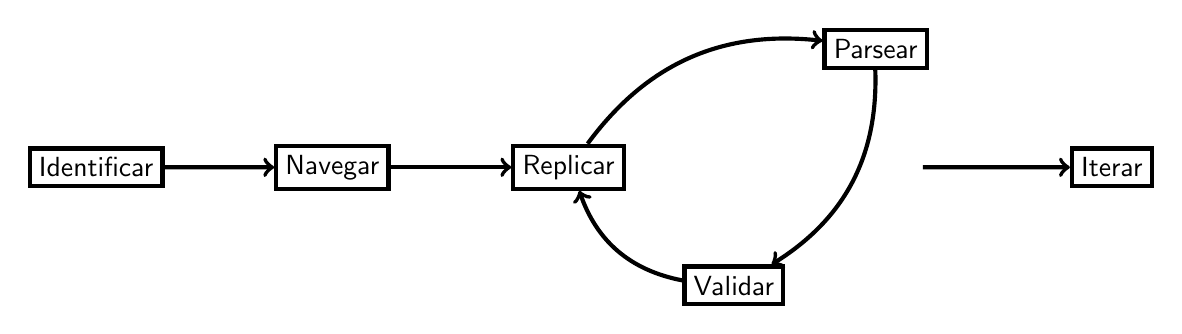
\begin{tikzpicture}[scale = 3, line width = 1.5pt]
\draw
    (1,1) node[ draw](a1){Identificar}
    (2,1) node[ draw](a2){Navegar}
    (3,1) node[ draw](a3){Replicar}
    (4.3,1.5) node[ draw](a4){Parsear}
    (3.7,0.5) node[draw](a5){Validar}
    (5.3,1) node[ draw, line width = 1.5](a6){Iterar};
    
    \draw [->] (a1) -- (a2) node[midway,below] {};
    \draw [->] (a2) -- (a3) node[midway,above] {};
    \draw[->] (4.5,1) -- (a6);
    
    \path[->] (a5) edge [bend left = 30] node[left, red] {} (a3);
    \path[->] (a3) edge [bend left = 30] node[left, red] {} (a4);
    \path[->] (a4) edge [bend left = 30] node[left, red] {} (a5);
                                                                                                                                                                                                                                                                                                                                                                                                                                                                                                                                            
\end{tikzpicture}

    \fonte{Elaboração própria}
    \label{fig:webscraping}
\end{figure}

A possibilidade da reprodução de algorítimos por meio de \textit{web scraping} nos permite -- por vezes -- realizarmos coletas volumosas de dados da internet, como por exemplo, dados econômicos estruturados e não-estruturados. 

O \textit{web scraping} cada vez mais vem sendo utilizado no mundo empresarial e em políticas públicas. A partir deste, é possível monitorar atividades em tempo real, bem como variações de preços ou acontecimentos políticos de forma automatica.

De forma mais generalizada, exemplos de aplicações do \textit{web scraping} podem ser dados como: 1 - \textbf{área comercial e de vendas}, visto que é possível qualificar base de dados de maneira automática bem como adicionar informações às mesmas - como informações de clientes, ou algo que possa interessar; 2 - \textbf{monitorar preços de concorrência}, manter listado e atualizado a preços reais variações de preços, bem como lista de vendas de setores específicos; 3 - \textbf{\textit{marketing} e investigação de mercado}, investigar compradores, tendências, monitorar marcas. Neste ponto, o \textit{web scraping} pode ser utilizado para - desde a monitoração de fóruns \textit{onlines} até - investigações de tendências em redes sociais \cite{web2019utilidade}.

\subsection{O Fluxo de Funcionamento do \textit{web scraping}}

Utilizando termos mais técnicos, o funcionamento do \textit{web scraping} é baseado num fluxo partindo da identificação dos dados a serem coletados; a \textit{navegação} web; um fluxo interativo (replicação, \textit{parseamento} e validação); e finalmente a Iteração dos dados.\cite{web2019}

O primeiro passo, quando nos referimos a identificação, é definirmos o que queremos coletar. No presente trabalho, o foco se restringe as atas do COPOM (\textit{minutes}), disponíveis em inglês. Definem-se as páginas no site do Banco Central, e a partir delas, busca-se as informações necessárias para a coleta.  \cite{costa2016ensaios}. Tendo identificado nosso objetivo, foi feita uma seleção das atas necessárias para o presente trabalho. Como o escopo do estudo foram as atas do ano de 2003 ao ano de 2018, por meio de um algorítimo\footnote{http://selectorgadget.com/} definimos onde deveríamos trabalhar. A replicação dos dados ocorre por meio de um script no software R, no qual realizamos todo o processo anterior, bem como o download das atas. A iteratividade realizada nos permite baixar todas as atas em formato pdf, bem como armazená-las para o estudo posterior.


%\subsection{Utilidades mais comuns do \textit{web scraping}}

\section{A Divergência de Kullback-Liebler}

Como partes das ferramentas estatísticas na análise de discrepâncias ou semelhanças entre variáveis aleatórias, foi proposto a divergência de Kullback-Liebler (K-L). É importante salientar que esta função é base na construção do critério de Akaike para escolhas de modelos - critério muito utilizado na esfera econométrica \cite{wooldridge2006introduccao, gujarati2011econometria}.

\subsection{A Divergência de Kullback-Liebler ou Entropia Relativa}

Sejam $f$ e $g$ as funções de densidade de duas variáveis aleatórias unidimensionais contínuas. A informação de K-L, para o caso contínuo, pode ser dada por: 
\begin{align} \label{kullbackliebler}
I(f, g) = \int f(x)\log\left(\frac{f(x)}{g(x)}\right) \quad dx,
\end{align}

\noindent
onde $\log$ representa o logaritmo natural. A notação $I(f, g)$ pode ser estabelecida como `` a informação perdida quando $g$ é usado para aproximar $f$''. Dessa forma, $I(f, g)$ é a distância de $g$ para $f$. Outra interpretação da divergência de K-L é em relação a uma medida de ineficiência: dado a distribuição $g$ quando a distribuição $f$ é verdadeira.
\noindent
Para o caso de distribuições discretas, teremos:
\begin{align} \label{kullbackdiscreta}
I(f, g) = \sum_{i=1}^{k} p(x_{i}) \cdot \log\left( \frac{p(x_{i})}{q(x_{i})}\right),
\end{align}

\noindent
onde a verdadeira probabilidade do \textit{inésimo} termo é dada por $p(x_{i})$ enquanto $q(x_{i})$ constitui a distribuição de probabilidades aproximadas. %Neste caso, teríamos: $0 < p_i < 1$, $0 < \pi < 1$ e desta forma: $\sum p_i = \sum \pi_i = 1$. Assim, $f$ e $g$ corresponderiam a $p_i$ e $\pi_i$ respectivamente \cite[p. 51]{burnham2002practical}.

Caso distribuições iguais, teríamos $I(f,g) = 0 \iff p_i = q_i$. A medida de K-L, contextualizada como uma distância entre dois modelos - isso é, a discrepância entre eles  \cite[p. 51]{burnham2002practical}..

\subsection{Exemplos de K-L}

Podemos ilustrar a distância de K-L ($I(f, g)$) simulando distribuições. Seja $f$ uma distribuição Gamma com parâmetros de forma $\alpha$ e escala $\beta$ iguais a 4; isto é $\alpha = 4$ e $\beta = 4$. Consideraremos, então, 4 distribuições $g_i$, cada uma com 2 parâmetros: distribuição Weibull; Lognormal; gaussiana inversa; e F de Fisher-Snedecor (Tabela \ref{ref:tabeladist}) \cite[p. 54]{burnham2002practical}.

\begin{table}[!h]
\centering
\caption{Distribuições para comparação}
\begin{tabular}{lllc}
\hline
      & Modelo Aproximado                                            & $I(f, g_i)$ & Ordem \\ \hline
$g_1$ & Distribuição Weibull ($\alpha = 2, \beta = 20$)              & 0.046189    & 1     \\
$g_2$ & Distribuição Lognormal ($\theta = 2, \sigma^2 = 2$)          & 0.672316    & 2     \\
$g_3$ & Gaussiana Inversa ($\alpha = 16, \beta = 64$)                & 0.059960    & 3     \\
$g_4$ & Distribuição F de Fisher-Snedecor ($\alpha = 4, \beta = 10$) & 5.745504    & 4     \\ \hline
\end{tabular}
\fonte{Elaboração própria}
\label{ref:tabeladist}
\end{table}

De acordo com a Tabela \ref{ref:tabeladist}, a distribuição simulada que mais se aproxima da Gamma -- dado os parâmetros -- é a distribuição de Weilbul, seguido pela gaussiana inversa. Na Figura \ref{figcompa} apresentamos as distribuições de probabilidades comparadas na Tabela \ref{ref:tabeladist}.
\begin{figure}[!h]
    \centering
    \caption{Gráficos de gamma comparado às distribuições}
    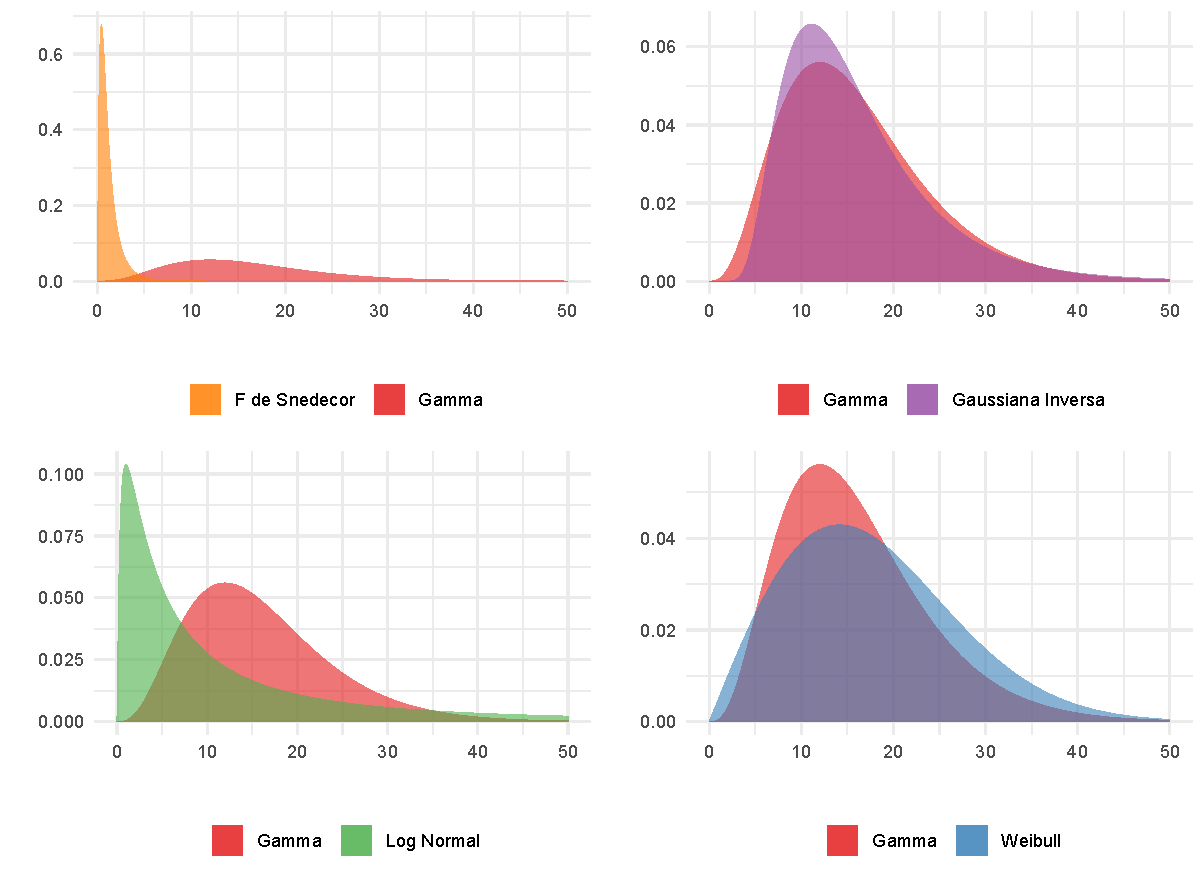
\includegraphics[width=\textwidth, height=10cm]{capitulos/figures/grafgamma.pdf}
    \fonte{Elaboração própria}
    \label{figcompa}
\end{figure}

%Na Figura \ref{figcompa} apresentamos as distribuições de probabilidades comparadas na Tabela \ref{ref:tabeladist}.
Supondo duas distribuições $f$ e $g$ normais $N(\Theta, \tau^2)$ e $N(\mu, \sigma^2)$ respectivamente. Se $E_f$ é a esperança referente a $f$ e a moda de um exemplo mais qualitativo, ou analítico, considere que $f$ é a densidade de uma distribuição normal $\mathbb{N}(\Theta, \tau^2)$.

\subsection{K-L para Distribuições Normais}
\label{normal}

Supondo duas distribuições $f$ e $g$ normais $N(\Theta, \tau^2)$ e $N(\mu, \sigma^2)$ respectivamente. Se $E_f$ é a esperança referente a $f$ e a moda de um exemplo mais qualitativo, ou analítico, considere que $f$ é a densidade de uma distribuição normal $\mathbb{N}(\Theta, \tau^2)$.

Seja $X$ uma variável aleatória governada por uma normal uniforme $N(\mu, \sigma^2)$. Isto é $X \sim N(\mu, \sigma^2)$, observamos que se denotarmos a esperança referente a $f$, $E_f$ temos: 
\begin{align*}
    E_f[(X - \mu)^2] &= E_f[(X - \Theta)^2 + 2(X - \Theta)(\Theta - \mu) + (\Theta - \mu)^2]\\
                     &= \tau^2 + (\Theta - \mu)^2
\end{align*}
então, para uma distribuição normal $g(x) = (2\pi\sigma^2)^{-\frac{1}{2}}\exp\{-(x - \mu)^2 / (2\sigma^2)\}$, temos:
\begin{align*}
    E_f[\log g(X)] &= E_f\left[\frac{1}{2}\log(2\pi\sigma^2)-\frac{(X-\mu)^2}{2\sigma^2}\right]\\
                   &= -\frac{1}{2}\log(2\pi\sigma^2) - \frac{\tau^2 + (\Theta - \mu)^2}{2\sigma^2}
\end{align*}
e, particular, se considerarmos $\mu = \Theta$ e $\sigma^2 = \tau^2$ nessa expressão, teremos:
\begin{align*}
    E_f[\log f(x)] = -\frac{1}{2}\log(2\pi\tau^2) - \frac{1}{2}
\end{align*}
assim, a distância de K-L de $f$ em relação a $g$ é dada por (\ref{kullbackliebler}):
\begin{align*}
    I(f,g) &= E_f[\log g(X)] - E_f[\log f(X)]\\
           &= \frac{1}{2}\left\{\log\frac{\sigma^2}{\tau^2} + \frac{\tau^2 + (\Theta - \mu)^2}{\sigma^2} - 1 \right\} \quad ,
\end{align*}

\noindent
a Figura \ref{fig:normal}, apresenta a variação de $I(f,g)$ dado que $\sigma^2 = 1$ e $\mu = 0$. $y$ representa $\tau$ e $x$ representa $\Theta$, da última equação. Na escala, os valores aproximados para a divergência de K-L.

\begin{figure}[!h]
    \centering
    \caption{Comparações de $I(f,g)$ quando $\Theta$ e $\tau$ variam, assumindo uma normal padrão ($N(0, 1)$)}
    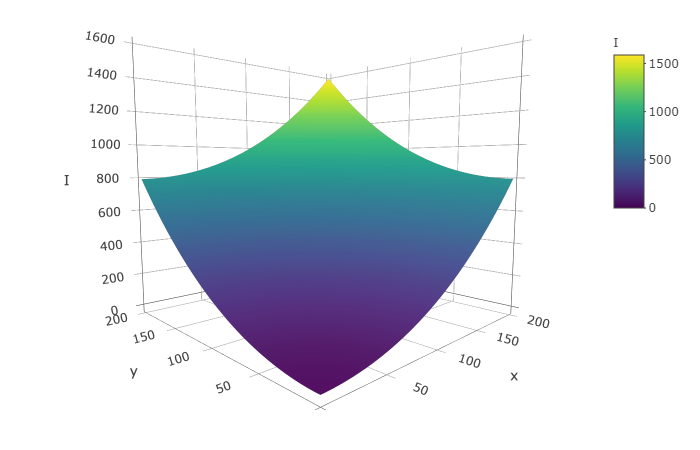
\includegraphics[width=.8\textwidth]{capitulos/figures/plot3d.png}
    \fonte{Elaboração própria}
    \label{fig:normal}
\end{figure}

\subsection{K-L para Modelos Normais e de Laplace}
\label{laplace}

Assumimos desta vez que $f$ segue uma distribuição de Laplace, tal que $f(x) = \frac{1}{2}\exp(-|x|)$ e $f(x) = N(\mu, \sigma^2)$. Neste caso nós teríamos:
\begin{align*}
    E_f[\log f(X)] &= -\log 2 - \frac{1}{2}\int_{-\infty}^{\infty}|x|e^{-1|x|}dx\\
                   &= -\log 2 - \frac{1}{2}\int_{-\infty}^{\infty}xe^{-x}dx\\
                   &= -\log 2 -1,\\
    E_f[\log g(X)] &= -\frac{1}{2}\log(2\pi\sigma^2) - \frac{1}{4\sigma^2}\int_{-\infty}^{\infty}(x - \mu)^2e^{-|x|}dx\\
                   &= -\frac{1}{2}\log(2\pi\sigma^2) - \frac{1}{4\sigma^2}(4 + 2\mu^2).
\end{align*}
então, a divergência de K-L é dada por:
\begin{align*}
    I(f,g) = \frac{1}{2}\log(2\pi\sigma^2) + \frac{2 + \mu^2}{2\sigma^2} - \log 2 - 1.
\end{align*}

\begin{figure}[!h]
    \centering
    \caption{Valores da divergência de K-L para uma distribuição normal-laplace, dado $\mu = 0$}
    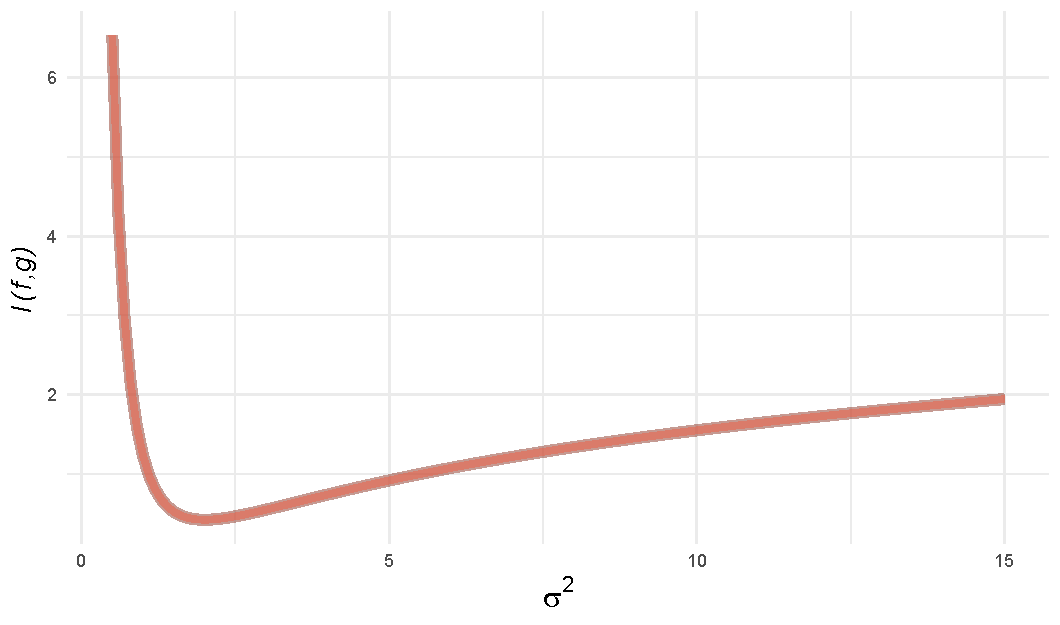
\includegraphics[width=.8\textwidth]{capitulos/figures/kllaplace.pdf}
    \fonte{Elaboração própria}
    \label{fig:laplacesomente}
\end{figure}


Na Figura (\ref{fig:laplacesomente}), apresentamos a variação de $I(f,g)$, assumindo $\mu=0$. Em ambos os casos, podemos variar os parâmetros (nas distribuições normais, fixar $\sigma$ e permitir a variação de $\tau$ e $\Theta$, e em relação ao normal laplace, permitir a variação de $\sigma$ e $\mu$)

\section{Índice de \textit{Otimismo}}

Analisar o que um texto expressa não necessariamente é algo simples. Automatizar este processo, além disso, pode ser algo bem custoso. A questão fundamental de uma analise de sentimentos é saber o que uma frase; texto; quer -- essencialmente -- expressar. Esta técnica nos permite identificar, por exemplo, a polaridade de um texto, se esse se manifesta de forma mais positiva ou negativa. É possível, além disso, contabilizar as palavras mais ditas num \textit{corpus} - ou num conjunto de textos, bem como suas distribuições de frequências. 

A partir do momento que possuímos um texto, precisamos tratá-lo. Existem técnicas diferentes para esse tratamento. Neste trabalho, utilizamos dicionários de \textit{stopwords}. Isso é, dado um texto qualquer, removemos \textbf{todas as palavras} contidas num dicionário de \textit{stopwords}. 

É comum que em qualquer que seja o \textit{corpus}, possuamos palavras que \textit{de forma geral} não contribuiriam de maneira nenhuma para entendermos o que o texto está expressando. De forma geral, dicionários de \textit{stopwords} estão em inglês - bem como os dicionários léxicos - e então somos forçados a trabalhar com textos em inglês\footnote{O COPOM disponibiliza suas atas em inglês (minutes)}. Geralmente, palavras de um dicionário de \textit{stopwords} concentram-se em palavras como ``\textit{the}'', ``\textit{and}'', ``\textit{these}'',``\textit{of}'' (Tabela \ref{tab:stopwords}). Esta tabela contém exemplos de palavras de um dicionário de \textit{stopwords} disponível no pacote \textbf{tidytext} \cite{tidystop} disponível para a linguagem R. Este dicionário apresenta três dicionários léxicos de \textit{stopwords}, o \textbf{onix}; o \textbf{SMART} e o \textbf{snowball}\footnote{http://www.lextek.com/manuals/onix/stopwords1.html, http://www.jmlr.org/papers/volume5/lewis04a/lewis04a.pdf, http://snowball.tartarus.org/algorithms/english/stop.txt}. 

\begin{table}[!h]
\centering
\caption{Exemplos de palavras de um dicionário de \textit{stopwords}}
\begin{tabular}{lllllll}
  \hline
 a & across & all & also & and & anyway & are \\ 
 a's & actually & allow & although & another & anyways & aren't \\ 
 able & after & allows & always & any & anywhere & around \\ 
 about & afterwards & almost & am & anybody & apart & as \\ 
 above & again & alone & among & anyhow & appear & aside \\ 
 according & against & along & amongst & anyone & appreciate & ask \\ 
 accordingly & ain't & already & an & anything & appropriate & asking \\ 
   \hline
\end{tabular}
\fonte{Elaboração própria}
\label{tab:stopwords}
\end{table}

Neste trabalho, utilizaremos a análise de sentimentos para montarmos um índice simples de otimismo, configurado da seguinte forma \cite{costa2016ensaios}:

\begin{align} \label{indice} 
    I_O &= \frac{N_P}{N_P + N_N} \quad ,
\end{align}

\noindent
isso é, em \ref{indice} representamos que o valor do índice é dado pelo número total de palavras positivas ($N_P$) dividido pela soma do número total de palavras positivas mais o número total de palavras negativas ($N_N$). Ainda, de tal forma que $0 \leq I_O \leq 1$.  

A classificação das palavras, é feita, entretanto, por meio de um dicionário léxico. Dicionários léxicos, na maioria das vezes, são dicionários criados por instituições de pesquisa que visam classificar palavras com valores de forma - ou não - categórica. Dessa maneira, a cada palavra é atribuído um valor ou uma característica. 

A Tabela \ref{tab:lexico} apresenta palavras de um dicionário léxico proposto por \citeonline{hu2004mining} de polaridade contido no pacote \textbf{qdapDictionaries} \cite{qdapdict}, parte do \textit{software R}. Neste exemplo, o dicionário visa classificar uma palavra de forma positiva ou negativa, tal que $palavra = -1$ se negativa ou $palavra = 1$ se positiva.

\begin{table}[!h]
\centering
\caption{Exemplos de palavras de um dicionário léxico}
\begin{tabular}{rlrlrlr}
  \hline
 & \textbf{Palavra} & \textbf{Valor} & \textbf{Palavra} & \textbf{Valor} & \textbf{Palavra} & \textbf{Valor} \\ 
  \hline
1 & a plus & 1.00 & abomination & -1.00 & abrade & -1.00 \\ 
  2 & abnormal & -1.00 & abort & -1.00 & abrasive & -1.00 \\ 
  3 & abolish & -1.00 & aborted & -1.00 & abrupt & -1.00 \\ 
  4 & abominable & -1.00 & aborts & -1.00 & abruptly & -1.00 \\ 
  5 & abominably & -1.00 & abound & 1.00 & abscond & -1.00 \\ 
  6 & abominate & -1.00 & abounds & 1.00 & absence & -1.00 \\ 
   \hline
\end{tabular}
\fonte{Elaboração própria}
\label{tab:lexico}
\end{table}

\section{Vetor Auto-regressivo}

O surgimento dos modelos auto-regressivos são oriundos da década de 80, como alternativa às críticas dos grandes números de restrições impostas às estimações pelos modelos estruturais \citeonline{var2012bcb}. 

\begin{citacao}
``A ideia era desenvolver modelos dinâmicos com o mínimo de restrições, nos quais todas as variáveis econômicas
fossem tratadas como endógenas. Sendo assim, os modelos VAR examinam relações lineares entre cada variável e os valores defasados dela própria e de todas as demais variáveis, impondo como restrições à estrutura da economia somente: a escolha do conjunto relevante de variáveis e do número máximo de defasagens envolvidas nas relações entre elas.'' \cite[p.1]{var2012bcb}
\end{citacao}

\noindent
matematicamente, é possível representar um modelo VAR de primeira ordem (VAR(1)) da seguinte forma:
\begin{align} \label{var1}
\begin{split}
    y_{1t} &= \delta_1 + \phi_{11}y_{1,t-1} + \phi_{12}y_{2,t-1} + u_{1t} \\
    y_{2t} &= \delta_2 + \phi_{21}y_{1,t-1} + \phi_{22}y_{2,t-1} + u_{2t}
\end{split}
\end{align}

\noindent
onde $y_1$ e $y_2$ são variáveis endógenas e $u_1$ e $u_2$ são os erros para cada equação. $\phi_{12}$ por sua vez representa a dependência linear de $y_{11}$ em $y_{2, t-1}$ na presença de $y_{1, t-1}$ - isso é, representa o efeito condicional de $y_{2, t-1}$ sobre $r_{1t}$, dado $y_{1, t-1}$. Dessa forma, se $\phi_{12} = 0$, então $y_{1t}$ não depende de $y_{2, t-1}$. De forma análoga, se $\phi_{21}=0$, então a segunda equação mostra que $y_{2t}$ não depende de $y_{1, t-1}$ quando $y_{2, t-1}$ é dado. Ainda, podemos representar o sistema \ref{var1}, da seguinte forma:
\begin{align*}
\begin{bmatrix}
    y_{1t} \\
    y_{2t}
\end{bmatrix}
&=
\begin{bmatrix}
    \delta_1 \\
    \delta_2 \\
\end{bmatrix}
+
\begin{bmatrix}
    \phi_{11} & \phi_{21} \\
    \phi_{12} & \phi_{22} \\
\end{bmatrix}
\begin{bmatrix}
    y_{1,t-1} \\
    y_{2,t-1} \\
\end{bmatrix}
+
\begin{bmatrix}
    u_{1t} \\
    u_{2t} \\
\end{bmatrix}
\end{align*}



\noindent
ou, de acordo com as definições apropriadas \cite[p.322]{verbeek2008guide}:
\begin{align*}
    \Vec{Y}_t = \phi + \Theta \Vec{Y}_{t-1} + \Vec{\epsilon_t} 
\end{align*}

\noindent
onde $\Vec{Y}_t=[ y_{1t}, y_{2t}]'$ e $\Vec{\epsilon_t}=[u_{1t}, u_{2t}]'$. Isso estende um modelo auto-regressivo de primeira ordem para um caso de \textit{mais dimensões}. De forma geral, um VAR(p) para um vetor k-dimensional pode ser dado por:
\begin{align*}
    \Vec{Y}_t = \phi + \Theta_1 \Vec{Y}_{t-1} + \dots + \Theta_p \Vec{Y}_{t-p} + \Vec{\epsilon}_t
\end{align*}
\noindent
onde cada $\Theta_j$ é uma matriz $k \times k$ e $\Vec{\epsilon}_t$ é um vetor de comprimento $k$ de ruídos brancos (\textit{white noises}), com matriz de covariância $\sum$. No caso \textit{univariado}, poderíamos definir a matriz polinomial a partir do operador de defasagem:
\begin{align*}
    \Theta(L) = I_k - \Theta_1 L - \dots - \Theta_p L^p
\end{align*}
\noindent
sendo $I_k$ uma matriz identidade $k$. Logo, poderíamos escrever o VAR como:
\begin{align*}
    \Theta(L)\Vec{Y}_t = \phi + \Vec{\epsilon}_t.
\end{align*}
\noindent
a matriz \textit{lag} polinomial é uma matriz $k \times k$, onde cada elemento corresponde a ordem $p$ num polinômio $L$

O modelo VAR implica um modelo ARMA para cada um de seus componentes. As vantagens em se considerar os componentes de forma simultânea é que o modelo acaba por ser mais parcimonioso, inclui menos defasagens, e possibilita previsões mais precisas, visto que o conjunto de informações é estendido para incluir também o histórico das outras variáveis \cite[p.322]{verbeek2008guide}. Por uma outra perspectiva, \citeonline{sims1980macroeconomics} afirma que o uso de modelos VAR ao invés de equações simultâneas estruturais é vantajoso, isso porquê a distinção entre variáveis exógenas e endógenas não tem que ser feita \textit{a priori} e de restrições `arbitrária' não são necessárias.    

\section{Função de impulso resposta} \label{respostaimpulso}

Da mesma forma que é possível representar um auto-regressivo a partir do seu componente de média móvel, podemos escrever um VAR como um vetor de média móvel (VMA). A representação de um VMA tem funcionalidade essencial na metodologia de \citeonline{sims1980macroeconomics}, a qual permite traçarmos as diferentes projeções dado choques nas variáveis contidas no VAR. Considerando a representação matricial de um VAR(1), temos:
\begin{align} \label{var1mat}
\begin{bmatrix}
    y_{1t} \\
    y_{2t}
\end{bmatrix}
=
\begin{bmatrix}
    \delta_1 \\
    \delta_2 \\
\end{bmatrix}
+
\begin{bmatrix}
    \phi_{11}y_{1,t-1} \\
    \phi_{12}y_{1,t-1} \\
\end{bmatrix}
+
\begin{bmatrix}
    \phi_{21}y_{2,t-1} \\
    \phi_{22}y_{2,t-1} \\
\end{bmatrix}
+
\begin{bmatrix}
    u_{1t} \\
    u_{2t} \\
\end{bmatrix}    
\end{align}

\noindent
podemos representar da seguinte forma:
\begin{align} \label{var2mat}
\begin{bmatrix}
    y_{1t} \\
    y_{2t}
\end{bmatrix}
=
\begin{bmatrix}
    \overline{y_1} \\
    \overline{y_2} \\
\end{bmatrix}
+ \sum_{i=0}^{\infty}
\begin{bmatrix}
    \phi_{11} & \phi_{12} \\
    \phi_{21} & \phi_{22}\\
\end{bmatrix}^i
\begin{bmatrix}
    u_{1t-i} \\
    u_{2t-i} \\
\end{bmatrix}
\end{align}

\noindent
a equação (\ref{var2mat}) expressa $y_{1t}$ e $y_{2t}$ em termos de \{$u_{1t}$\} e \{$u_{1t}$\} respectivamente. Podemos, entretanto -- e ainda -- reescrever (\ref{var2mat}) em termos de \{$u_{y_1t}$\} e \{$u_{y_2t}$\}. Assim, o vetor de erros pode ser escrito como \cite{enders2008applied}:
\begin{align} \label{var3mat}
\begin{bmatrix}
    u_{1t} \\
    u_{2t}
\end{bmatrix}
= \frac{1}{1 - b_{12}b_{21}}
\begin{bmatrix}
    1 & -b_{12} \\
    -b_{21} & 1 \\
\end{bmatrix}
\begin{bmatrix}
    u_{y_1t} \\
    u_{y_2t}\\
\end{bmatrix}
\end{align}

\noindent
combinando (\ref{var2mat}) e (\ref{var3mat}), temos:
\begin{align*} 
\begin{bmatrix}
    y_{1t} \\
    y_{2t}
\end{bmatrix}
=
\begin{bmatrix}
    \overline{y_1} \\
    \overline{y_2} \\
\end{bmatrix}
+ \frac{1}{1 - b_{12}b_{21}} \sum_{i=0}^{\infty}
\begin{bmatrix}
    \phi_{11} & \phi_{12} \\
    \phi_{21} & \phi_{22}\\
\end{bmatrix}^i
\begin{bmatrix}
    1 & -b_{12} \\
    -b_{21} & 1 \\
\end{bmatrix}
\begin{bmatrix}
    u_{y_1t} \\
    u_{y_2t}\\
\end{bmatrix}
\end{align*}

\noindent
ainda, para simplificar a notação, substituiremos a matriz 2 $\times$ 2, tal que:

\begin{align*}
\Gamma_i = \frac{A_1^i}{1 - b_{12}b_{21}}
\begin{bmatrix}
    1 & -b_{12} \\
    -b_{21} & 1 \\
\end{bmatrix}
\end{align*}

\noindent
consequentemente, a representação de média móvel apresentada em (\ref{var2mat}) e (\ref{var3mat}) pode ser escrita em termos de $u_{y_1t}$ e $u_{y_2t}$:
\begin{align} 
\begin{bmatrix}
    y_{1t} \\
    y_{2t}
\end{bmatrix}
=
\begin{bmatrix}
    \overline{y_1} \\
    \overline{y_2} \\
\end{bmatrix}
+ \sum_{i=0}^{\infty}
\begin{bmatrix}
    \Gamma_{11} (i) & \Gamma_{12} (i) \\
    \Gamma_{21} (i) & \Gamma_{22} (i)\\
\end{bmatrix}^i
\begin{bmatrix}
    u_{y_1t} \\
    u_{y_2t} \\
\end{bmatrix}
\end{align}
\noindent
ou de forma mais compacta:
\begin{align} \label{mediamovel}
    x_t = \epsilon + \sum_{i=0}^{\infty}\Gamma_i u_{t-1}
\end{align}

A representação apresentada em (\ref{mediamovel}) é uma ferramenta extremamente útil para examinar interações entre as variáveis $y_1$ e $y_2$. os coeficientes de $\Gamma_i$ podem ser utilizados para gerar efeitos de $u_{y_1t}$ em choques de $u_{y_1t}$ para períodos de tempo de $y_t$ e $y_2$. Dessa forma, é possível visualizar que os quatro elementos $\Gamma_{jk}(0)$ são \textbf{multiplicadores de impacto} \cite[p.295]{enders2008applied}.

Os efeitos acumulados de um impulso em  $u_{y_1t}$ e/ou $u_{y_2t}$ podem ser obtidos pela soma apropriada dos coeficientes das \textit{funções de resposta impulso}. Por exemplo,podemos perceber que, depois de $n$ períodos o efeito de $u_{y_2t}$ no valor de $y_{1 + n}$ é $\Gamma_{12}(n)$. Assim, depois de $n$ períodos a soma acumulada dos efeitos de $u_{y_2t}$ em $y_1$ é
\begin{align*}
    \sum_{i=0}^n \Gamma_{12}(i)
\end{align*}

\noindent
se $y_1$ e $y_2$ são estacionárias, os valores de $\Gamma_{jk}(i)$ converge para zero, quanto maior $i$ for. Assim, \textit{os choques não podem ter efeitos permanentes em séries estacionárias}. Disso segue que:
\begin{align*}
    \sum_{i=0}^\infty \Gamma_{jk}^2(i)  \text{ é finito}
\end{align*}

\noindent
os quatro conjuntos de coeficientes $\Gamma_{11}(i)$, $\Gamma_{12}(i)$, $\Gamma_{21}(i)$ e $\Gamma_{22}(i)$ são chamados de \textbf{função de resposta impulso}.


\chapter{Resultados Obtidos} \label{capitulo4}

O objetivo deste capítulo é apresentar os resultados obtidos a partir da metodologia desenvolvida no capítulo \ref{metodologia}. É realizado um exercício prático que visa melhor entender as expressões que as reniões do banco central desejam transmitir por meio das atas. Utilizaremos, entretanto, suas versões em inglês (\textit{minutes}), devido ao fato de não haver dicionários léxicos em português que permita um tratamento às atas.

O trabalho feito aqui é referente ao período de 2003-2018. Que por sua vez compete da gestão Meirelles à gestão Ian Goldfajn frente ao BCB -- do governo Lula ao governo Temer. Vale salientar, além disto, o \textit{software}/linguagem de programação utilizado: este trabalho foi feito exclusivamente por meio da linguagem R \cite{cran}. Sua escolha foi devido a esta linguagem ser considerada moderna e de alto nível, possibilitando de forma simples uma análise robusta dos dados. Ainda, por ser uma linguagem de programação voltada para estatística, como no próprio manual ``feita por estatísticos, para estatísticos'', o R possibilita uma vasta gama de opções para análise textual e de dados. Os códigos deste capítulo, bem como deste trabalho estão disponíveis no \href{https://github.com/gustavovital/Monografia}{repositório online da monografia} \url{https://github.com/gustavovital/Monografia}.

\section{Base de dados}

De acordo com o período analisado, de 2003 à 2018, foram disponibilizadas 140 atas do BCB das respectivas reuniões. Dessa forma, totaliza-se 140 reuniões do COPOM. A partir de um algoritmo de \textit{web scraping}, acessamos essas atas e fizemos download, das suas correspondentes em inglês (\textit{minutes}).

O período escolhido é relacionado com as mudanças políticas e econômicas no Brasil, levando em consideração, também, o tamanho amostral, afim de compreendermos melhor o que se passou nesses anos.

%\subsection{Obtenção da Base de Dados}

%Como dito anteriormente, foi utilizado um algoritmo de \textit{web scraping} para a obtenção das atas do COPOM. 

Inicialmente, por meio do pacote \textit{rvest} \cite{rvest} descobrimos as URL's referentes as atas do COPOM - isso é, de todas. Feito isto, obtemos as URL's por meio do pacote ``\textbf{cronoAno a}''\footnote{http://selectorgadget.com/}, bem como obtemos os links das atas.

Por meio de uma estrutura de repetição simples armazenamos estas atas em listas e realizamos os \textit{downloads} das atas, já do período selecionado, 2003-2018 . Armazenamos estas num diretório.

Utilizando o pacote \textit{tm} \cite{tm}, fazemos a leitura dos PDF's e criamos um \textit{dataframe} que contém os \textit{corpus}\footnote{Efetivamente os textos que iremos trabalhar neste \textit{corpus}, contém basicamente os caracteres das leituras dos PDF's} das atas. Nosso \textit{dataframe} fica com três colunas (numero da ata, nome do PDF, e \textit{corpus}) e 140 linhas (cada uma referente a uma ata). 

Para cada \textit{corpus} contido no documento aplicamos uma técnica de \textit{stop words}, por meio do dicionário \textit{stopwords} \cite{tidystop}, e adicionamos palavras que julgamos ser desnecessárias, assumindo que tal palavra aparece \textit{pelo menos} 400 vezes no total dos corpus. Dentre as palavras que desconsideramos, podemos citar como exemplo numerais ou nomes próprios sem relevância para uma análise econômica. Além disso, removemos palavras com erro de leitura devido a quebra de linhas (por exemplo \texttt{ninflation})\footnote{As palavras com erro de leitura foram desconsideradas nesta parte do processo. Na contagem geral de palavras, passamos a considerar, por essas poderem interferir no resultado final.}.
\begin{figure}[!h]
    \centering
    \caption{Núvem de palavras das palavras que mais aparecem nas atas do COPOM durante todo o período analisado}
    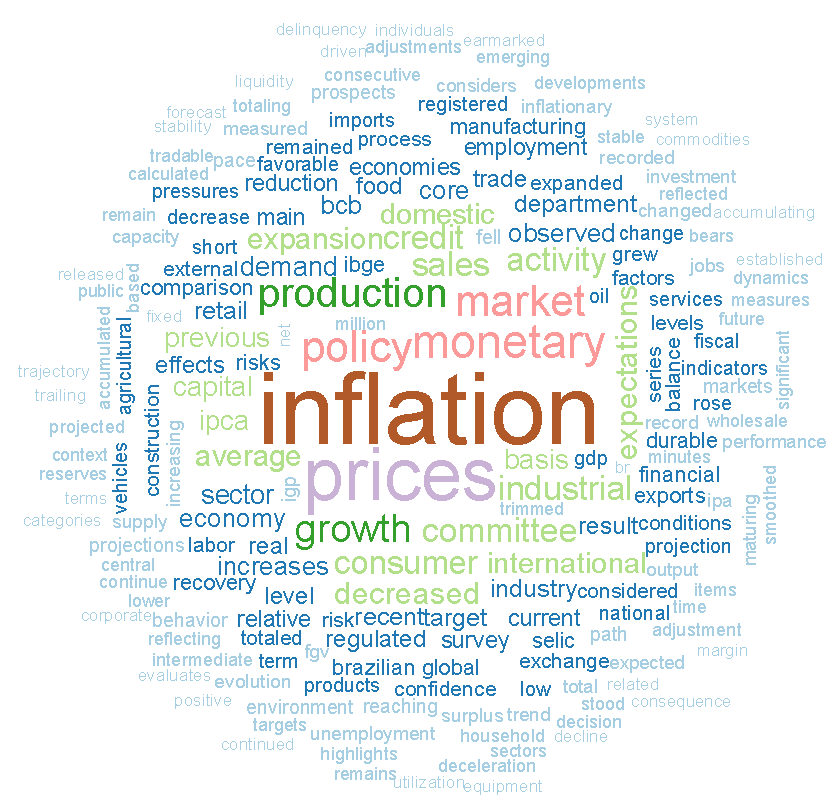
\includegraphics[width=.8\textwidth]{capitulos/figures/wordcloud.pdf}
    \fonte{BCB. Elaboração própria}
    \label{fig:wc01}
\end{figure}

A Figura \ref{fig:wc01} apresenta em escala as palavras que mais aparecem nas atas do COPOM, levando em consideração a técnica aplicada de \textit{stopwords}. Nitidamente, nos atentamos ao fato de \textbf{inflation}, \textbf{prices}, e \textbf{market} tomarem o primeiro plano, quanto a nossa atenção às palavras mais recorrentes.

\subsection{Estatísticas Descritivas}

O primeiro \textit{dataframe} de análise que obtemos diz respeito as frequências das palavras de cunho econômico. Feito isso, é interessante uma contagem das palavras. Na Tabela \ref{tab:contgeral}, podemos ver as palavras que mais aparecem nas atas do COPOM no período estudado. Ainda, devemos salientar:  essa é a contagem ``\textbf{líquida}'' das palavras - isso é, já foi feita a correção relativa às palavras repetidas ou não contabilizadas\footnote{Por exemplo, na contagem bruta, teríamos levado em consideração palavras como \textit{nprices, price} e \textit{nprices}}. 

\begin{table}[!h]
\centering
\caption{Palavras que mais aparecem nas atas do COPOM (2003-2018)}
\begin{tabular}{ll|ll|ll|ll}
\hline
Palavra    & n    & Palavra      & n    & Palavra       & n    & Palavra   & n    \\ \hline
inflation  & 7370 & committee    & 1785 & decreased     & 1579 & capital   & 1279 \\
prices     & 5079 & industrial   & 1785 & expansion     & 1468 & ipca      & 1256 \\
monetary   & 2882 & sales        & 1778 & average       & 1433 & demand    & 1221 \\
policy     & 2651 & credit       & 1775 & international & 1427 & sector    & 1187 \\
market     & 2562 & consumer     & 1701 & domestic      & 1364 & economy   & 1166 \\
production & 2373 & activity     & 1698 & previous      & 1327 & observed  & 1159 \\
growth     & 2194 & expectations & 1593 & basis         & 1316 & increases & 1157 \\ \hline
\end{tabular}
\label{tab:contgeral}
\end{table}

Dito isso, pode-se, também, apresentar a contagem das palavras referente aos períodos específicos analisados. As Tabelas \ref{tab:contmeir}, \ref{tab:conttom}, e \ref{tab:contian} apresentam essas contagens.

\begin{table}[h]
\centering
\caption{Palavras que mais aparecem nas atas do COPOM (período Meirelles)}
\begin{tabular}{llllllll}
  \hline
Palavra & n & Palavra & n & Palavra & n & Palavra & n \\ 
  \hline
inflation & 4348 & industrial & 1329 & consumer & 1033 & activity & 926 \\ 
prices & 3212 & growth & 1272 & expansion & 983 & domestic & 926 \\ 
market & 1595 & policy & 1259 & average & 977 & expectations & 907 \\ 
production & 1559 & sales & 1211 & ipca & 935 & previous & 871 \\ 
monetary & 1395 & credit & 1162 & basis & 932 & capital & 864 \\ 
   \hline
\end{tabular}
\label{tab:contmeir}
\end{table}

\begin{table}[h]
\centering
\caption{Palavras que mais aparecem nas atas do COPOM (período Tombini)}
\begin{tabular}{llllllll}
  \hline
Palavra & n & Palavra & n & Palavra & n & Palavra & n \\ 
  \hline
inflation & 2377 & growth & 903 & activity & 607 & sector & 500 \\ 
  prices & 1781 & committee & 844 & credit & 605 & bcb & 492 \\ 
  monetary & 995 & production & 813 & sales & 567 & expansion & 477 \\ 
  policy & 960 & decreased & 754 & industry & 564 & observed & 475 \\ 
  market & 919 & consumer & 663 & international & 526 & changed & 473 \\ 
   \hline
\end{tabular}
\label{tab:conttom}
\end{table}

\begin{table}[!h]
\centering
\caption{Palavras que mais aparecem nas atas do COPOM (período Goldfajn)}
\begin{tabular}{llllllll}
  \hline
Palavra & n & Palavra & n & Palavra & n & Palavra & n \\ 
  \hline
inflation & 645 & expectations & 246 & brazilian & 156 & easing & 117 \\ 
  monetary & 492 & risks & 211 & baseline & 153 & projections & 117 \\ 
  policy & 432 & activity & 165 & balance & 126 & governor & 116 \\ 
  committee & 429 & department & 165 & central & 119 & process & 116 \\ 
  economy & 306 & evolution & 165 & adjustments & 118 & risk & 116 \\ 
   \hline
\end{tabular}
\label{tab:contian}
\end{table}

Trivialmente, percebemos que a palavra que mais aparece nas atas é \textit{inflation}. O controle da inflação frente a meta para a inflação é um dos pontos de interesse do BC, além disso temos que levar em consideração o crescimento da inflação ao final do governo Dilma. \textit{Price} deixa de aparecer como uma palavra importante nas atas da gestão Goldfajn e \textit{policy} não aparece nas atas referentes ao governo Lula.

A partir da contagem total das palavras\footnote{O \textit{dataframe} referente possui mais de 12.000 palavras identificadas, dentre as quais considera-se numeral como um caractere} devemos definir nosso objeto de estudo. Trabalharemos com as 10 palavras de cunho econômico que mais aparecem nas atas do COPOM.

Alguns pontos têm que ser considerados. Primeiramente, esse estudo prevê um período de 16 anos, um total de 140 atas. Entretanto, os períodos de gestão do BCB não foram regulares, e mesmo que fossem, não poderíamos supor que o número de atas por período seria o mesmo, bem como os tamanhos das atas.

\subsection{Frequência das Principais Palavras}

Das 140 atas que utilizamos, no período Lula (gestão Meirelles) temos um total de 76 atas; no período Dilma (gestão Tombini) temos um total de 45 atas; por fim, no período Temer (gestão Goldfajn) temos um total de 19 atas. Ainda, a partir das 10 palavras \textit{de cunho econômico} que mais aparecem nas atas do COPOM, podemos fazer um estudo dirigido para cada período. Inicialmente, vamos considerar os valores \textit{absolutos} das palavras - isso é, a simples contagem de quantas vezes cada palavra aparece, independentemente do tamanho da ata\footnote{Ver repositório online}. 

As palavras que mais aparecem em cada período, como já exposto anteriormente, se encontram nas Tabelas \ref{tab:contmeir}, \ref{tab:conttom}, e \ref{tab:contian}. Podemos, agora, ilustrar, por meio de um histograma, suas distribuições; e um gráfico de linha, para em relação às ocorrências das palavras.

Inicialmente, como feito na seção anterior, faremos isso para todos os períodos (2003-2018)\footnote{Ver repositório online}. A distribuição das palavras acaba por não seguir um distribuição identificável visualmente. Nos histogramas, podemos notar isso quando em relação aos \textit{kernels} apresentados. As figuras estão disponíveis no repositório da Monografia.

\subsection{Frequências Relativas}

Como é possível perceber, se fossemos trabalhar com as ocorrências das palavras de forma \textit{absoluta}, teríamos um problema notável: como os tamanhos das atas variam, não poderíamos comparar as ocorrências das palavras de forma direta. Desta forma, como metodologia utilizada, passaremos a considerar as frequências relativas das palavras em relação a cada ata.

Basicamente, a metodologia utilizada foi, dado o número de ocorrências de uma palavra, divide-se este número pelo total de palavras nas atas - já desconsiderado as palavras de dicionários de \textit{stopwords}, tal que:
$$Fp_i = \frac{p_i}{N_i}$$
\noindent
em que $Fp_i$ é a frequência da palavra $p$, dada por $\frac{p_i}{N_i}$; ou seja, o número de ocorrências da palavra $p$, dividido pelo número total de ocorrência de todas as palavras $N$, na ata $i$.

Podemos perceber um tendência principal nas palavras \textit{inflation} e \textit{monetary}, possivelmente relacionada com a conjuntura econômica que o país vivia - crise econômica acentuada em 2015. Enquanto, por exemplo, \textit{prices}, \textit{industrial}, \textit{credit}, \textit{growth}, \textit{consumer}, e \textit{market} praticamente deixam de aparecer no período Goldfajn - por vezes nem aparecem, se referem somente ao responsável da sessão, no BC, isso é não há nenhuma interpretação econômica para essas palavras nas atas no período pós-impeachment

É possível ainda, sugerir uma interpretação econômica para o desaparecimento dessas palavras. Se analisarmos o caso das palavras \textit{monetary} e \textit{policy}, percebemos que a correlação das frequências dessas palavras é de \texttt{0.973746}, nos dando um indício de que essas são utilizadas conjuntamente, em \textit{monetary policy} - de tal forma que isso indique que o andamento dessas palavras se refira ao tratamento com a política monetária\footnote{Não utilizamos essa técnica de trabalho neste documento. Se fosse o objetivo trabalhar com conjuntos de palavras, trabalharíamos com \textit{clusters}}.  

\begin{figure}[!h]
    \centering
    \caption{Comparação das frequências de \textit{Monetary} e \textit{Policy}}
    \includegraphics[width=\textwidth]{capitulos/figures/policy_monetary_ggplot.pdf}
    \fonte{BCB. Elaboração própria}
    \label{fig:monetarypolicy}
\end{figure}

A Figura \ref{fig:monetarypolicy} apresenta as frequências relativas às atas das palavras \textit{monetary} e \textit{policy} no decorrer do período analisado. Nitidamente, é possível verificar uma correlação dessas duas palavras. 

\begin{figure}[!h]
    \centering
    \caption{Comparação das frequências de \textit{Monetary} e \textit{Policy} com o IPCA acumulado em 12 meses}
    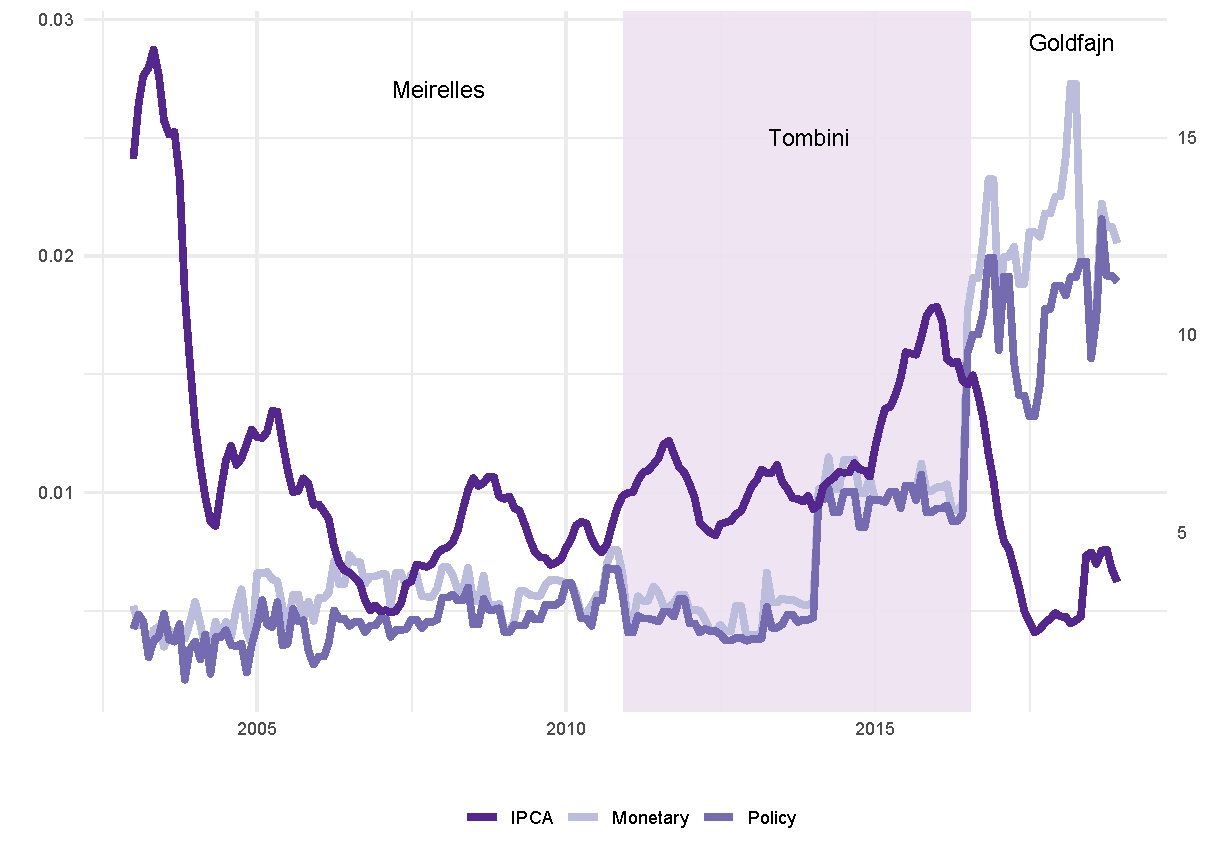
\includegraphics[width=\textwidth]{capitulos/figures/graficoipcapolicy.pdf}
    \fonte{BCB. Elaboração própria}
    \label{fig:monpolipca}
\end{figure}

A Figura \ref{fig:monpolipca} apresenta a evolução do ipca acumulado em 12 meses de acordo com os períodos de gestão do BCB, isso é: o aumento em relação a frequência do aparecimento das palavras \textit{policy} e \textit{monetary} pode estar relacionado com uma possível ênfase a mudança de política monetária adotada pelo BC. A partir de 2015 há um \textit{boom} na inflação acumulada, sendo o tratamento dessa uma prioridade, faz sentido que se espere uma mudança em relação à política monetária, se esta não estiver surtindo efeito.

\section{A divergência de Kullback-Liebler nas frequências das Atas do COPOM}

Como primeiro exercício prático deste trabalho, é proposto o cálculo da divergência de K-L. Isso é, verificaremos se as expressões das atas nos períodos analisados possuem similaridades com base nas 148 palavras que mais aparecem no conjunto dos 140 \textit{minutes} do COPOM. Num primeiro momento, a intenção foi o cálculo das 200 palavras que mais aparecem nas atas, entretanto, durante o período Goldfajn algumas palavras deixam de aparecer\footnote{As palavras que deixam de aparecer nas atas são: sales, basis, capital, industry, comparison, ibge, exports, durable, manufacturing, expanded, grew, series, construction, totaled, rose, oil, registered, agricultural, imports, products, vehicles, igp, surplus, jobs, recorded, record, output, ipa, fgv, maturing, intermediate, household, smoothed, totaling, calculated, bears, million, trimmed, tradable, liquidity, driven, trailing, br, categories, evaluates, earmarked, equipment, individuals, net, delinquency, commodities, fixed}, já como um indício de mudança em relação a abordagem de política monetária e -- assim -- não seria possível o cálculo da divergência de K-L. 

Como o tamanho das atas variam de período a período analisado -- bem como de ata para ata -- foi necessário trabalharmos com a frequência relativa dessas palavras.

%A diferença de K-L é uma medida, dentro do campo da teoria da informação, capaz de mensurar o quanto uma distribuição $f(x)$ é \textit{próxima} a uma distribuição $g(x0)$. Como apresentado no capítulo \ref{metodologia}, para o caso discreto, esta é calculada da seguinte forma:
%\begin{align*}
%I(f, g) = \sum_{i=1}^{k} p(x_{i}) \cdot \log\left( \frac{p(x_{i})}{q(x_{i})}\right)
%\end{align*}
%\noindent
%a fim de aplicarmos essa medida de distância, podemos considerar a equação da seguinte forma: 1 - considerando $f(x)$ a distribuição para as atas do período Meirelles e $g(x)$ para o período Goldfajn, teríamos que a divergência de K-L seria dada como o somatório das distribuições das palavras do período Meirelles multiplicado pelo logaritmo natural da diferença das distribuições de palavras do período Meirelles pela distribuições de palavras do período Goldfajn.

É sabido que a política monetária adotada pelos períodos Meirelles e Tombini foram políticas monetárias sobre vigência do \textit{Partido dos Trabalhadores} (PT); por um outro lado, durante o período Goldfajn, o partido vigente foi o Partido do Movimento Democrático Brasileiro (PMDB). É esperado então que haja uma similaridade maior em relação aos períodos Meirelles-Tombini do que, por exemplo, os períodos Meirelles-Goldfajn. Ainda, podemos assumir uma possível transição de política monetária no que diz respeito ao período Tombini -- dessa forma, consideramos as distribuições de palavras, ou expressão das atas, levando em consideração três períodos distintos de política brasileira: Meirelles (Lula), Tombini (Dilma), e Goldfajn (Temer).

\subsection{Análise para os Períodos de Gestão do Banco Central}

Essa subseção é dividida em três partes. Na primeira faremos uma análise levando em consideração como distribuição das palavras tomando como referência o período Meirelles, na segunda o período Tombini, e por fim o período Goldfajn. Isso é necessário pois a medida de informação de K-L não é uma medida simétrica, logo quando analisada tomando como referência o período Meirelles contra, por exemplo o período Tombini, não teríamos o mesmo resultado quando tomando o período Tombini como referência. Ao final é apresentado uma tabela geral com os valores da divergência de K-L para as 10, 20, 50, 100, e 148 palavras.

\subsubsection*{Período Meirelles}

A primeira comparação feita é em relação ao período Meirelles. Tomando a distribuição de palavras desse período como referência, é calculado o valor da divergência de K-L em comparação aos outros dois períodos: Tombini e Goldfajn.

\begin{figure}[!h]
    \centering
    \caption{Divergência de K-L conforme o acréscimo de palavras para o cálculo (período Meirelles)}
    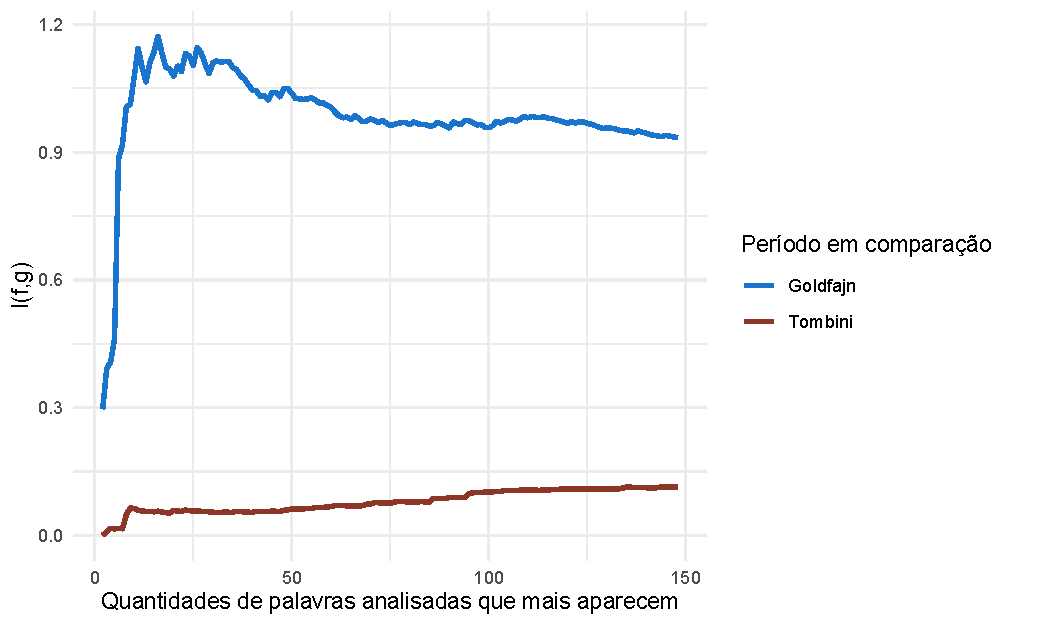
\includegraphics[width=\textwidth]{capitulos/figures/klmeirelles.pdf}
    \fonte{Elaboração própria.}
    \label{fig:klmeirelles}
\end{figure}

A Figura \ref{fig:klmeirelles} apresenta a evolução da divergência de K-L conforme o acréscimo das palavras que mais aparecem nas atas. Nitidamente, as distribuições de palavras do período Meirelles se aproxima da distribuições de palavras do período Tombini de forma mais expressiva do que do período Goldfajn, com uma diferença mínima próxima a 0.3 no valor do critério de K-L.

\subsubsection*{Período Tombini}

Tomando a distribuição de palavras do período Tombini como referência, é calculado o valor da divergência de K-L em comparação aos outros dois períodos: Meirelles e Goldfajn.

\begin{figure}[!h]
    \centering
    \caption{Divergência de K-L conforme o acréscimo de palavras para o cálculo (período Tombini)}
    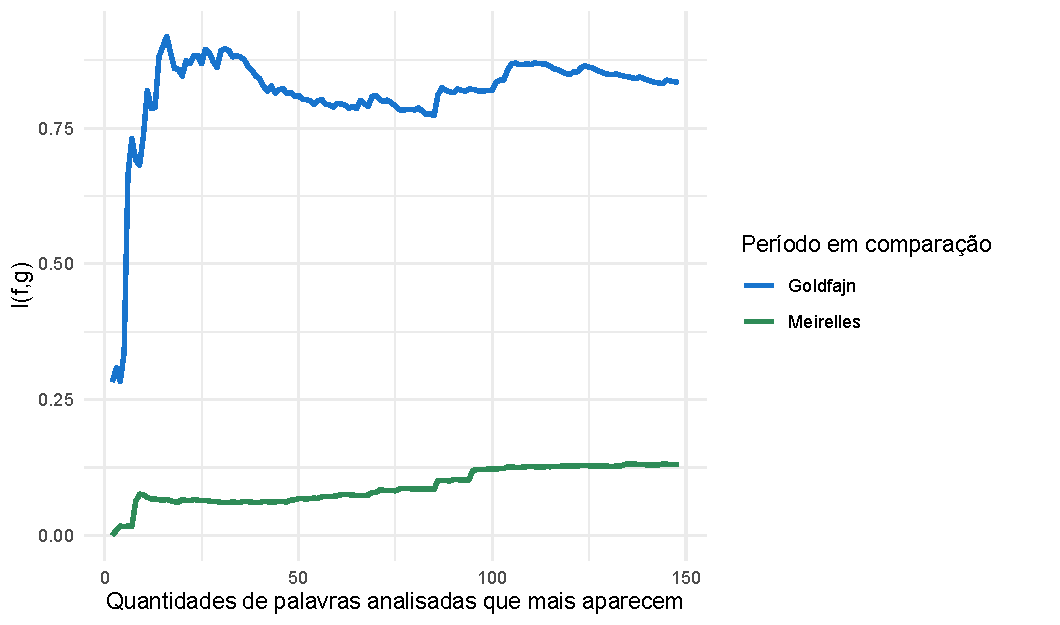
\includegraphics[width=\textwidth]{capitulos/figures/kltombini.pdf}
    \fonte{Elaboração própria.}
    \label{fig:kltombini}
\end{figure}

A Figura \ref{fig:kltombini} apresenta, então, a evolução da divergência de K-L conforme o acréscimo das palavras que mais aparecem nas atas quando tomamos por referência o período Tombini. Nitidamente, as distribuições de palavras desse período analisado se aproxima da distribuições de palavras do período Meirelles de forma mais expressiva -- novamente -- do que do período Goldfajn, com uma diferença mínima próxima a 0.25 no valor do critério de K-L.

É enfatizado, então, uma semelhança quando as distribuições de palavras estão contidas num período de mesma gestão política vigente (PT); enquanto quando comparado ao período político PMDB as distribuições se tornam mais distantes.

\subsubsection*{Período Goldfajn}

Por fim, analisa-se como período de referência a gestão Goldfajn. Então, é feita uma comparação frente aos outros dois períodos: período Meirelles e período Tombini.

Como já apresentado, é esperado que essa distribuição de palavras seja mais distinta à distribuição de palavras da gestão Meirelles -- consequentemente mais próxima a gestão Tombini.

\begin{figure}[!h]
    \centering
    \caption{Divergência de K-L conforme o acréscimo de palavras para o cálculo (período Tombini)}
    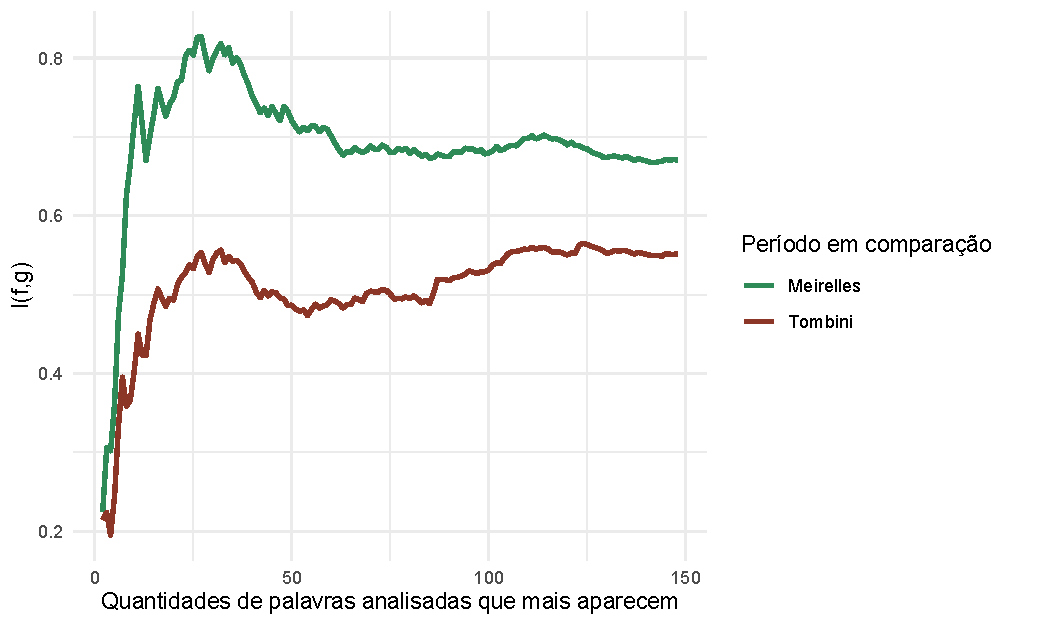
\includegraphics[width=\textwidth]{capitulos/figures/klgoldfajn.pdf}
    \fonte{Elaboração própria.}
    \label{fig:klgoldfajn}
\end{figure}

De fato, a Figura \ref{fig:klgoldfajn} demonstra que ainda que as distâncias das distribuições tenham sido reduzidas (quando o período Goldfajn é referência), elas ainda indicam uma proximidade maior ao período Tombini do que ao período Meirelles.

De forma geral, podemos apresentar os resultados das Figuras \ref{fig:klmeirelles}, \ref{fig:kltombini} e \ref{fig:klgoldfajn} como um indicador do que acontece frente as expressões das atas no que diz repeito ao âmbito de política monetária. Isso é, no período Meirelles a distribuição de palavras realmente se assemelha mais ao período Tombini e menos ao período Goldfajn. Seja pela própria política monetária ou mesmo em relação ao âmbito de um outro cenário macroeconômico.

Uma outra abordagem que pode ser levada em consideração é em relação aos termos econômicos. Conforme o número de palavras nas distribuições aumentam a tendência é que menos palavras sejam relacionadas a questão econômica/conjuntural vigente em um determinado período.

Se nos atentarmos as dez palavras mais recorrentes, teremos -- em ordem: \textit{inflation, prices, market, production, monetary, industrial, growth, policy, sales,} e \textit{credit}. Entretanto, e obviamente, de \textbf{todas} as palavras analisadas, nem todas são referentes às questões econômicas de forma \textit{direta}. Por exemplo, ainda entre as palavras mais recorrentes em todo o período analisado podemos perceber palavras como \textit{previous} e \textit{observed} -- que obviamente estão relacionadas a termos econômicos, mas não são termos econômicos em si. 
\newpage

\begin{table}[] 
\caption{Valores de $I(f,g)$ para diferentes números de palavras utilizadas para o cálculo}
\begin{tabular}{l|l|l|l|l|l}
\hline
\multicolumn{6}{c}{Período Referente: Meirelles}                                                  \\ \hline
                   & \multicolumn{5}{l}{$N^o$ de palavras mais recorrentes utilizadas para o cálculo} \\ \cline{2-6} 
Período comparado & 10             & 20            & 50            & 100          & 148          \\ \hline
Tombini            & 0.063          & 0.058         & 0.062         & 0.1          & 0.11         \\
Goldfajn           & 1.1            & 1.1           & 1             & 0.96         & 0.94         \\ \hline
\multicolumn{6}{c}{Período Referente: Tombini}                                                    \\ \hline
                   & \multicolumn{5}{l}{$N^o$ de palavras mais recorrentes utilizadas para o cálculo} \\ \cline{2-6} 
Período comparado & 10             & 20            & 50            & 100          & 148          \\ \hline
Meirelles          & 0.074          & 0.066         & 0.068         & 0.12         & 0.13         \\
Goldfajn           & 0.74           & 0.85          & 0.81          & 0.82         & 0.84         \\ \hline
\multicolumn{6}{c}{Período Referente: Goldfajn}                                                   \\ \hline
                   & \multicolumn{5}{l}{$N^o$ de palavras mais recorrentes utilizadas para o cálculo} \\ \cline{2-6} 
Período comparado & 10             & 20            & 50            & 100          & 148          \\ \hline
Meirelles          & 0.72           & 0.75          & 0.72          & 0.68         & 0.67         \\
Tombini            & 0.4            & 0.49          & 0.49          & 0.53         & 0.55         \\ \hline
\end{tabular}
\label{tabelageral}
\fonte{Elaboração própria}
\end{table}

A Tabela \ref{tabelageral} apresenta os diferentes valores das distâncias de K-L para diferentes números de palavras utilizados para o cálculo da divergência de K-L. De forma quase genérica, quanto maior o número de palavras utilizadas para o cálculo, maior o valor da divergência.


\section{Índices de Otimismo  e Expressões das Atas}

O objetivo, agora, deste trabalho é apresentar um possível índice de otimismo. Como apresentado no capítulo \ref{metodologia}, o índice de otimismo consiste \textit{basicamente} em considerar o numero de palavras positivas identificadas nas atas dividido pelo número total de palavras positivas e negativas contidas nestas, como segue na Equação (\ref{indicecosta}).

Para criarmos este índice é necessário algumas mudanças na série das atas. Como se sabe, as reuniões do BC não são/foram sempre regulares em relação as datas. Isto é, não temos um série regular de tempo. A metodologia utilizada foi transformar esta série em mensal - normalmente o COPOM se reúne oito vezes por ano, desta forma o que foi feito foi considerar o último valor observado do índice referente à ata da reunião. Para a contagem das palavras, foi utilizado o dicionário do pacote \textit{qdap} do R \cite{qdapdict}, e a partir dele realizamos a soma das palavras positivas e negativas em cada ata - por fim, de todas as atas.

Como dito anteriormente, o \textit{score} do índice varia de 0 a 1, dessa forma é possível verificarmos uma possível correlação entre o índice e a situação conjuntural brasileira.

\begin{table}[!h] 
\centering
\caption{Exemplo de \textit{scores} e contagem de palavras positivas e negativas}
\begin{tabular}{llll}
\hline
       & \multicolumn{2}{l}{Palavras}               & \multirow{2}{*}{Score} \\ \cline{2-3}
       & \multicolumn{1}{l|}{Positivas} & Negativas &                        \\ \hline
ATA 80 & 66                             & 58        & 0.532                  \\
ATA 81 & 73                             & 59        & 0.553                  \\
ATA 82 & 53                             & 69        & 0.434                  \\
ATA 83 & 39                             & 51        & 0.472                  \\ \hline
\end{tabular} \label{scores1}
\fonte{Elaboração própria}
\end{table}

A Tabela \ref{scores1} apresenta um exemplo de \textit{score} para as atas 80 à 83. A partir dos \textit{scores} podemos definir momentos de otimismo e pessimismo para as atas dos COPOM. Isso é, dado que o índice varia de 0 a 1, quando o valor do \textit{score} é menor que 0.5, podemos determinar um período de pessimismo na ata; caso contrário, determina-se otimismo.

\begin{figure}[!h]
    \centering
    \caption{Índice de otimismo ao longo do período analisado}
    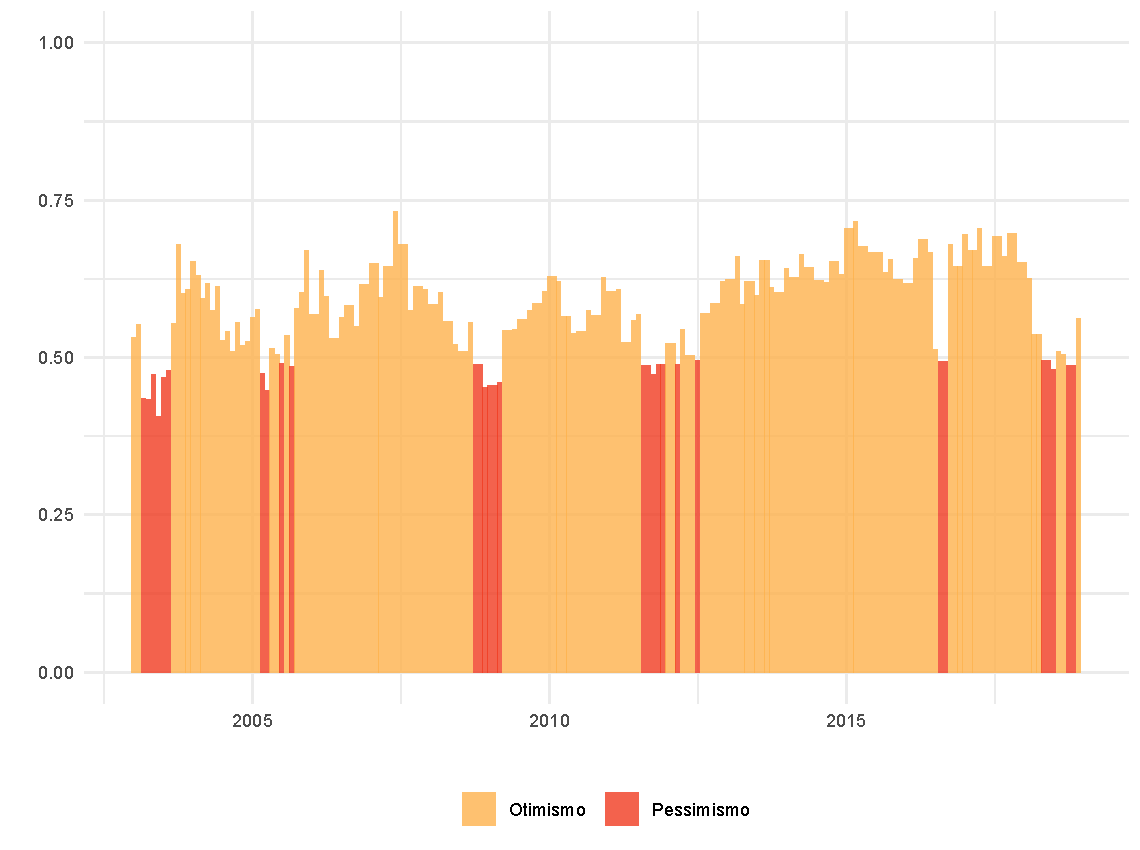
\includegraphics[width=\textwidth]{capitulos/figures/graf_indice_ggplot.pdf}
    \fonte{Elaboração própria}
    \label{fig:grafind}
\end{figure}


A Figura \ref{fig:grafind} apresenta a variação do índice proposto. Na barra abaixo da série é apresentado momentos de ``otimismo'' e ``pessimismo'' de acordo com o \textit{score}. De forma geral, percebe-se que o índice se mantem na maior parte do tempo de forma positiva - mesmo em momentos de crise. Argumenta-se que a abordagem do COPOM aos momentos críticos na conjuntura brasileira é dado de forma otimista. 

O índice de otimismo proposto pode ser utilizado como uma ferramenta de apoio à analise conjuntural brasileira, de tal forma que seria possível determinar a expressão do BCB para o período atual. Assim, este poderia servir como um indicador - \textit{proxy} - para o tipo de atuação do BCB frente a uma possível situação conjuntural mais crítica. 

\section{Exemplo de Aplicação}

Como proposto em \citeonline{shapiro2018measuring} e \citeonline{shapiro2019taking}, a partir de um índice de \textit{positividade} ou \textit{negatividade} é possível tentarmos entender o que aconteceria com a economia ou com esse índice, dados choques de algumas variáveis macroeconômicas.

Para entendermos o que poderia acontecer em alguns cenários, iremos nos basear em \citeonline{shapiro2019taking} e iremos reproduzir o exercício de função impulso resposta para algumas variáveis macroeconômicas brasileiras. Isso é, assumindo endogeneidade nas variáveis, estima-se um VAR para melhor compreender o que aconteceria se, por exemplo, num cenário de choque positivo no índice, como o Índice de Preços ao Consumidor Amplo (IPCA) acumulado em 12 meses reagiria. 

\subsection{Base de Dados e Período de Estimação}

Para a realização deste exercício, utilizaremos o IPCA acumulado em 12 meses, como uma \textit{proxy} da inflação acumulada; e o Índice de Atividade Econômica do Banco Central (IBC-Br) - com ajuste sazonal. respectivamente, representam as séries de número 13522 e 24364, do SGS - Sistema Gerenciador de Séries Temporais (BCB). Além dessas séries, utilizaremos, também, o índice proposto em (\ref{indice}). 

Uma primeira questão que nos toma, é se as séries são estacionárias. Para nos certificarmos da presença ou não de estacionariedade, utilizaremos o teste de Dickey-Fuller aumentado (ADF). Esse teste tem como hipótese nula ($H_0$) a presença de raiz unitária; usualmente, sua hipótese alternativa ($H_A$) é aceita como presença de estacionariedade - condição necessária para a estimação do VAR.  

\begin{table}[!h]
\centering
\caption{Testes de raiz unitárias para as variáveis utilizadas no exercício}
\begin{tabular}{llllc}
  \hline
Variáveis & ADF (-) & ADF (c) & ADF (ct) & Integração \\ 
  \hline
IbcBr & 1.9531 & -2.1196 & -0.7971 & I(1)\\ 
IPCA*** & -2.7598 & -4.3018*** & -4.1054*** & I(0) \\ 
Índice & -0.4107 & -3.7810*** & -3.9939*** & I(0)\\ 
D(IbcBr) & -7.4123*** & -7.6612*** & -7.8751*** & I(0)\\ 
D(IPCA) & -6.4765*** & -6.5740*** & -6.6907*** & I(0)\\ 
D(Índice) & -11.4768*** & -11.4444*** & -11.4429*** & I(0)\\ 
Est. de Teste (Tau) (10\%) & -1.6200 & -2.5700 & -3.1300 & -\\ 
Est. de Teste (Tau) (5\%) & -1.9500 & -2.8800 & -3.4300 & -\\ 
Est. de Teste (Tau) (1\%) & -2.5800 & -3.4600 & -3.9900 & -\\ 
   \hline
\end{tabular} \label{adf}
\fonte{Elaboração própria.}
\nota{* Rejeita-se a hipótese nula a nível de 10\%, ** Rejeita-se a hipótese nula a nível de 5\%, *** Rejeita-se a hipótese nula a nível de 1\%}
\end{table}

A Tabela \ref{adf} apresenta os resultados dos testes de raiz unitária realizados. De acordo com os testes realizados, podemos rejeitar a hipótese de presença de raiz unitária para todas as séries em diferença. Trabalhando em nível, entretanto, só podemos rejeitar esta hipótese para as séries IPCA e índice - mesmo assim, para as últimas duas séries, somente com presença de intercepto e tendência.

É necessário, desta forma, trabalharmos com a série \texttt{D(IbcBr)} - a série em diferênça do Índice de Atividade Econômica do Banco Central.

\subsection{O Modelo Estimado}

A partir do pacote \textit{vars} pode-se estipular a ordem do VAR, dado critérios de informação de akaike, Hannan-Quinn, e Bayesian Information Criterion; respectivamente AIC, HQ, e BIC \cite{pfaff2008var}. Foi verificado que para todos os critérios de informação apontaram para um VAR de segunda ordem. Isso é: foi regredido nas três variáveis utilizadas (D(IbcBr), IPCA, e índice) até a segunda ordem de defasagem de cada uma, de tal forma que o sistema de cada apresente 6 regressores. A equação estimada do VAR(2) para o indice, ficaria, então:
\begin{align*}
    indice_t = \Gamma_1 indice_{t-1} + \Gamma_2 indice_{t-2} &+ \Gamma_3 IPCA_{t-1} + \Gamma_4 IPCA_{t-2}\quad+ \\
                                                           & + \Gamma_5 \Delta IbcBr_{t-1} + \Gamma_6 \Delta IbcBr_{t-6} + const + trend + \epsilon
\end{align*}

\noindent
feito isso, e realizadas das estimações, pode-se estimar a função resposta ao impulso.

\subsection{Impulso Resposta ao Índice}
Como apresentado em (\ref{respostaimpulso}) em \citeonline{shapiro2019taking} e em \citeonline{jorda2005estimation}, realizamos o procedimento de estimação do VAR(2) e obtivemos suas funções de resposta ao impulso do índice.

\begin{figure}[!h]
    \centering
    \caption{Resposta das variáveis utilizadas a um choque em \textit{índice}}
    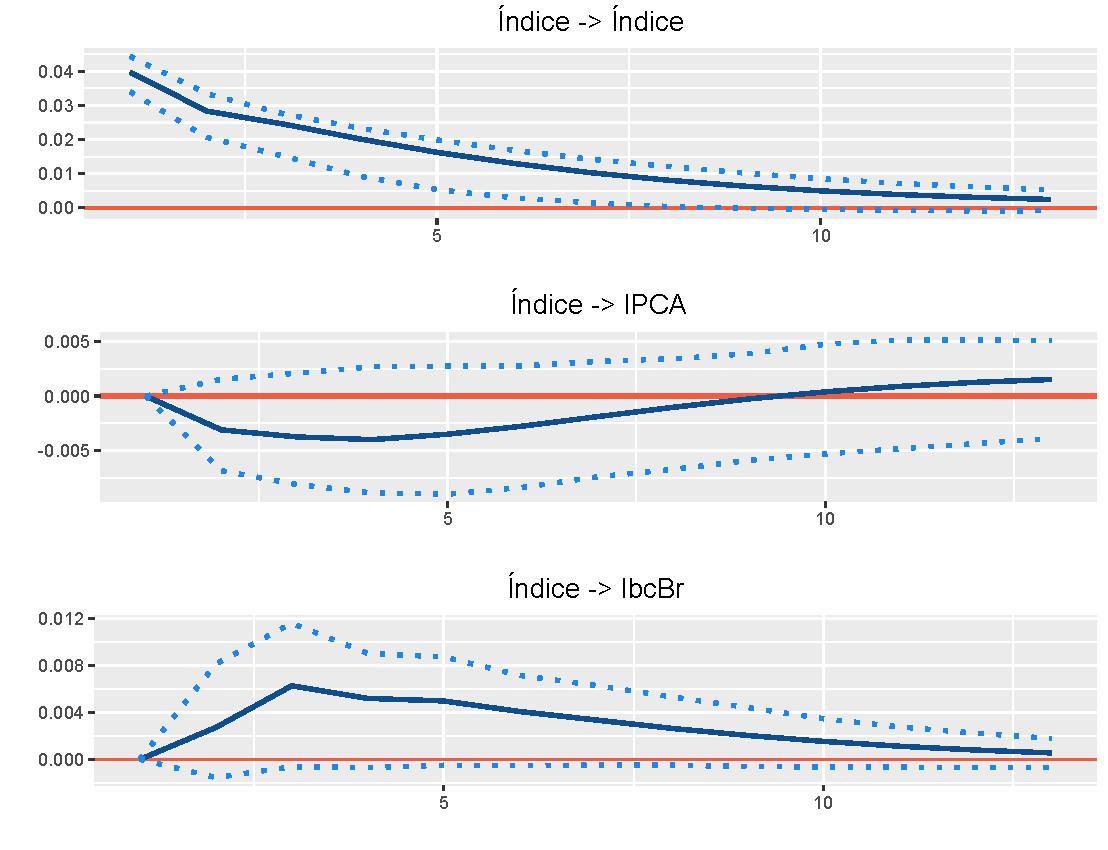
\includegraphics[width=.8\textwidth]{capitulos/figures/irf.pdf}
    \fonte{Elaboração própria}
    \label{fig:fri}
\end{figure}

A Figura \ref{fig:fri} apresenta a projeção para um choque em índice para um período posterior de 12 meses. Isto é, de acordo com a estimação, obtida a partir da \textit{identificação de cholesky} (ver \citeonline{enders2008applied}), dado um choque positivo no índice de otimismo obtido, a tendência de projeção seria que, para as variáveis obtidas:

\begin{enumerate}
    \item A varição do Índice de Atividade Econômica do Banco Central tenderia a ser positiva por um período de 12 meses a frente. Ainda, em cerca de 15 períodos esta voltaria ao seu estado original (não representado na figura);
    \item Em relação ao IPCA, o Índice de Preços ao Consumidor amplo sofreria uma queda inicial, em relação ao acumulado em 12 meses. Posteriormente, essa queda seria convertida em acréscimo, entretanto, com valor inferior a queda inicial. Após cerca de 17 períodos o valor do IPCA acumulado em 12 meses tenderia ao seu estado inicial (não representado na figura). 
\end{enumerate}

É válido salientar que há uma vasta opção de variáveis macroeconômicas brasileiras que poderiam ser utilizadas como referência para uma possível correlação com o índice de otimismo. Utilizamos o IPCA e o Ibc-Br como forma de aproximar o exercício da proposta inicial de \citeonline{shapiro2019taking}, visto que foram variáveis de escolhas próximas. Nada impede, entretanto, de utilizarmos outras variáveis como componentes do VAR - bem como nada impede a utilização de outras técnicas de estimação, ou mesmo testes para verificação de causalidade, por exemplo.






\chapter{Considerações Finais}

Nesta monografia apresentamos as técnicas de \textit{web scraping} conjuntamente com as ferramentas de análise de sentimentos aplicados à métodos quantitativos para melhor compreender as expressões das atas do COPOM.

A partir da análise realizada foi possível encontrar semelhanças e diferenças quanto às expressões das atas em relação a diferentes períodos de gestão de política monetária do Banco Central do Brasil.

Levando em consideração estatísticas descritivas e medidas estatísticas mais robustas, podemos considerar que houve -- de fato -- uma maior semelhança em relação às políticas monetárias do período PT (Meirelles e Tombini) do que do período PMDB (Goldfajn).

Através de algorítimos e técnicas de \textit{web scraping} e \textit{text mining} foram feitos os \textit{downloads} das atas do COPOM, e o \textit{corpus} foi tratado mediante dicionários e algorítimos de \textit{stopwords}.

Por meio de nuvens de palavras (\textit{wordclouds}) e tabelas descritivas, foram apresentados os termos mais utilizados em cada período, de 2003 à 2018 bem como a variação da divergência de Kullback-Liebler quando comparamos esses principais termos -- até finalmente chegarmos a conclusão de que para \textbf{todos} os períodos a divergência de K-L foi menor em relação a Meirelles-Goldfajn (qualquer que seja o período referência) do que para qualquer outro período analisado.

Ainda, foi proposto um índice de otimismo, baseado em \citeonline{costa2016ensaios} para uma melhor compreensão de como as reuniões do Comitê de Política Monetária se comportavam frente às variações do cenário macroeconômico brasileiro. Dessa forma, foi possível apresentar períodos de otimismo e de pessimismo para as reuniões do COPOM de 2003 à 2018, de acordo com os termos mais utilizados nas atas das reuniões periódicas do BCB.

Indo além, e com base na metodologia adotada por \citeonline{shapiro2019taking}, foi apresentado e estimado um VAR(2) bem como uma função de resposta ao impulso, apresentando uma relação de endogeneidade para o índice proposto, o Índice de Atividade Econômica do Banco Central e o IPCA acumulado em 12 meses. 

A função de resposta ao impulso indicou que mediante um choque positivo no índice de otimismo, o Índice de Atividade Econômica do Banco Central sofreria uma variação positiva; bem como dado esse mesmo choque, o IPCA acumulado em 12 meses sofreria uma variação negativa -- assim, afirmando um sentido econômico.

Dessa forma, foi possível concluir que quantificar dados textuais pode ser interessante no âmbito de entendermos como o Banco Central do Brasil se expressa, bem como compreender que essas expressões reafirmam uma tendência em relação à política monetária adotada em diferentes períodos -- seja quando essas reafirmam posições frente à variáveis macroeconômicas ou mesmo em relação a linha política adotada.  





% ----------------------------------------------------------
% ELEMENTOS PÓS-TEXTUAIS
% ----------------------------------------------------------
\postextual

% ----------------------------------------------------------
% Referências bibliográficas
% ----------------------------------------------------------

\bibliography{referencias}

%\begin{apendicesenv}
%\begin{landscape}
\chapter{Frequência de palavras de cunho econômico e distribuição das palavras} \label{anexoa}

\begin{longtable}{rrrrrrrrrrr}
\caption{Número de ocorrências das palavras de cunho econômico nas atas} \label{tab:long} \\
\hline
& inflation & prices & monetary & policy & market & production & growth & industrial & consumer & credit \\ \hline
\endfirsthead
 
\hline
& inflation & prices & monetary & policy & market & production & growth & industrial & consumer & credit \\ \hline
\endhead

\hline \multicolumn{11}{r}{{Continua na próxima página}} \\ \hline
\endfoot

\hline
\endlastfoot


ATA 80 & 29.00 & 42.00 & 11.00 & 9.00 & 12.00 & 5.00 & 6.00 & 6.00 & 8.00 & 4.00 \\ 
  ATA 81 & 39.00 & 55.00 & 10.00 & 11.00 & 19.00 & 2.00 & 6.00 & 10.00 & 10.00 & 5.00 \\ 
  ATA 82 & 43.00 & 59.00 & 10.00 & 10.00 & 18.00 & 3.00 & 6.00 & 7.00 & 10.00 & 2.00 \\ 
  ATA 83 & 33.00 & 43.00 & 6.00 & 6.00 & 14.00 & 10.00 & 3.00 & 7.00 & 10.00 & 8.00 \\ 
  ATA 84 & 40.00 & 50.00 & 9.00 & 8.00 & 14.00 & 10.00 & 5.00 & 11.00 & 12.00 & 7.00 \\ 
  ATA 85 & 66.00 & 70.00 & 11.00 & 10.00 & 15.00 & 6.00 & 7.00 & 11.00 & 16.00 & 10.00 \\ 
  ATA 86 & 59.00 & 71.00 & 10.00 & 14.00 & 22.00 & 10.00 & 6.00 & 12.00 & 15.00 & 10.00 \\ 
  ATA 87 & 53.00 & 48.00 & 11.00 & 10.00 & 17.00 & 5.00 & 8.00 & 13.00 & 8.00 & 7.00 \\ 
  ATA 88 & 43.00 & 56.00 & 12.00 & 11.00 & 16.00 & 13.00 & 14.00 & 9.00 & 11.00 & 6.00 \\ 
  ATA 89 & 48.00 & 43.00 & 11.00 & 12.00 & 15.00 & 12.00 & 4.00 & 14.00 & 7.00 & 13.00 \\ 
  ATA 90 & 37.00 & 44.00 & 11.00 & 6.00 & 19.00 & 10.00 & 15.00 & 15.00 & 9.00 & 16.00 \\ 
  ATA 91 & 36.00 & 39.00 & 12.00 & 9.00 & 20.00 & 7.00 & 22.00 & 10.00 & 7.00 & 13.00 \\ 
  ATA 92 & 62.00 & 63.00 & 16.00 & 11.00 & 28.00 & 5.00 & 17.00 & 19.00 & 16.00 & 16.00 \\ 
  ATA 93 & 53.00 & 33.00 & 12.00 & 8.00 & 26.00 & 13.00 & 18.00 & 20.00 & 9.00 & 10.00 \\ 
  ATA 94 & 67.00 & 63.00 & 11.00 & 13.00 & 21.00 & 14.00 & 16.00 & 21.00 & 19.00 & 14.00 \\ 
  ATA 95 & 50.00 & 47.00 & 9.00 & 6.00 & 22.00 & 14.00 & 14.00 & 15.00 & 8.00 & 1.00 \\ 
  ATA 96 & 56.00 & 58.00 & 14.00 & 12.00 & 32.00 & 11.00 & 15.00 & 23.00 & 13.00 & 12.00 \\ 
  ATA 97 & 49.00 & 60.00 & 10.00 & 10.00 & 25.00 & 5.00 & 15.00 & 12.00 & 8.00 & 10.00 \\ 
  ATA 98 & 51.00 & 48.00 & 13.00 & 12.00 & 27.00 & 7.00 & 18.00 & 18.00 & 12.00 & 16.00 \\ 
  ATA 99 & 44.00 & 57.00 & 12.00 & 11.00 & 26.00 & 8.00 & 19.00 & 19.00 & 9.00 & 17.00 \\ 
  ATA 100 & 75.00 & 68.00 & 19.00 & 13.00 & 26.00 & 12.00 & 23.00 & 23.00 & 14.00 & 13.00 \\ 
  ATA 101 & 42.00 & 61.00 & 18.00 & 11.00 & 32.00 & 3.00 & 21.00 & 24.00 & 15.00 & 9.00 \\ 
  ATA 102 & 34.00 & 68.00 & 12.00 & 7.00 & 18.00 & 7.00 & 13.00 & 24.00 & 10.00 & 11.00 \\ 
  ATA 103 & 42.00 & 71.00 & 12.00 & 12.00 & 25.00 & 8.00 & 25.00 & 21.00 & 11.00 & 11.00 \\ 
  ATA 104 & 51.00 & 70.00 & 21.00 & 14.00 & 28.00 & 10.00 & 22.00 & 24.00 & 11.00 & 12.00 \\ 
  ATA 105 & 59.00 & 73.00 & 23.00 & 19.00 & 22.00 & 25.00 & 26.00 & 22.00 & 17.00 & 16.00 \\ 
  ATA 106 & 55.00 & 61.00 & 21.00 & 14.00 & 26.00 & 9.00 & 17.00 & 18.00 & 16.00 & 11.00 \\ 
  ATA 107 & 61.00 & 53.00 & 22.00 & 15.00 & 29.00 & 25.00 & 17.00 & 31.00 & 16.00 & 11.00 \\ 
  ATA 108 & 65.00 & 54.00 & 21.00 & 18.00 & 23.00 & 21.00 & 25.00 & 15.00 & 14.00 & 11.00 \\ 
  ATA 109 & 51.00 & 57.00 & 16.00 & 11.00 & 20.00 & 17.00 & 27.00 & 16.00 & 13.00 & 12.00 \\ 
  ATA 110 & 49.00 & 62.00 & 13.00 & 11.00 & 22.00 & 21.00 & 14.00 & 21.00 & 18.00 & 16.00 \\ 
  ATA 111 & 68.00 & 61.00 & 19.00 & 17.00 & 21.00 & 24.00 & 24.00 & 17.00 & 15.00 & 14.00 \\ 
  ATA 112 & 62.00 & 67.00 & 20.00 & 16.00 & 21.00 & 23.00 & 28.00 & 20.00 & 18.00 & 15.00 \\ 
  ATA 113 & 73.00 & 81.00 & 16.00 & 16.00 & 18.00 & 27.00 & 12.00 & 22.00 & 19.00 & 4.00 \\ 
  ATA 114 & 69.00 & 64.00 & 18.00 & 11.00 & 20.00 & 26.00 & 7.00 & 27.00 & 14.00 & 14.00 \\ 
  ATA 115 & 54.00 & 54.00 & 15.00 & 9.00 & 20.00 & 15.00 & 13.00 & 19.00 & 12.00 & 14.00 \\ 
  ATA 116 & 57.00 & 53.00 & 18.00 & 10.00 & 24.00 & 23.00 & 10.00 & 22.00 & 14.00 & 16.00 \\ 
  ATA 117 & 49.00 & 49.00 & 19.00 & 12.00 & 19.00 & 14.00 & 14.00 & 16.00 & 16.00 & 17.00 \\ 
  ATA 118 & 47.00 & 49.00 & 24.00 & 17.00 & 28.00 & 12.00 & 22.00 & 15.00 & 11.00 & 14.00 \\ 
  ATA 119 & 45.00 & 46.00 & 21.00 & 16.00 & 26.00 & 14.00 & 15.00 & 6.00 & 10.00 & 13.00 \\ 
  ATA 120 & 55.00 & 52.00 & 27.00 & 16.00 & 26.00 & 21.00 & 12.00 & 25.00 & 9.00 & 17.00 \\ 
  ATA 121 & 50.00 & 61.00 & 28.00 & 18.00 & 22.00 & 27.00 & 8.00 & 28.00 & 10.00 & 17.00 \\ 
  ATA 122 & 54.00 & 59.00 & 24.00 & 16.00 & 21.00 & 26.00 & 9.00 & 22.00 & 11.00 & 15.00 \\ 
  ATA 123 & 64.00 & 69.00 & 28.00 & 19.00 & 29.00 & 39.00 & 15.00 & 19.00 & 14.00 & 22.00 \\ 
  ATA 124 & 73.00 & 66.00 & 28.00 & 20.00 & 26.00 & 33.00 & 17.00 & 20.00 & 11.00 & 23.00 \\ 
  ATA 125 & 71.00 & 54.00 & 24.00 & 18.00 & 38.00 & 35.00 & 28.00 & 18.00 & 8.00 & 23.00 \\ 
  ATA 126 & 68.00 & 60.00 & 30.00 & 19.00 & 32.00 & 37.00 & 23.00 & 19.00 & 8.00 & 26.00 \\ 
  ATA 127 & 67.00 & 70.00 & 27.00 & 19.00 & 35.00 & 40.00 & 25.00 & 21.00 & 14.00 & 6.00 \\ 
  ATA 128 & 76.00 & 72.00 & 31.00 & 22.00 & 31.00 & 37.00 & 24.00 & 19.00 & 11.00 & 20.00 \\ 
  ATA 129 & 79.00 & 54.00 & 25.00 & 19.00 & 39.00 & 38.00 & 21.00 & 17.00 & 16.00 & 30.00 \\ 
  ATA 130 & 74.00 & 62.00 & 26.00 & 21.00 & 40.00 & 41.00 & 18.00 & 19.00 & 17.00 & 28.00 \\ 
  ATA 131 & 73.00 & 57.00 & 27.00 & 21.00 & 34.00 & 32.00 & 25.00 & 18.00 & 15.00 & 25.00 \\ 
  ATA 132 & 79.00 & 59.00 & 32.00 & 26.00 & 36.00 & 31.00 & 27.00 & 17.00 & 16.00 & 32.00 \\ 
  ATA 133 & 84.00 & 58.00 & 31.00 & 27.00 & 33.00 & 29.00 & 27.00 & 17.00 & 15.00 & 31.00 \\ 
  ATA 134 & 91.00 & 62.00 & 29.00 & 27.00 & 31.00 & 32.00 & 26.00 & 19.00 & 19.00 & 28.00 \\ 
  ATA 135 & 94.00 & 72.00 & 33.00 & 29.00 & 33.00 & 34.00 & 21.00 & 20.00 & 19.00 & 28.00 \\ 
  ATA 136 & 86.00 & 76.00 & 27.00 & 22.00 & 32.00 & 46.00 & 36.00 & 21.00 & 23.00 & 25.00 \\ 
  ATA 137 & 88.00 & 75.00 & 33.00 & 28.00 & 32.00 & 36.00 & 38.00 & 20.00 & 17.00 & 29.00 \\ 
  ATA 138 & 87.00 & 84.00 & 28.00 & 27.00 & 36.00 & 37.00 & 28.00 & 21.00 & 21.00 & 26.00 \\ 
  ATA 139 & 77.00 & 75.00 & 29.00 & 28.00 & 34.00 & 40.00 & 30.00 & 26.00 & 24.00 & 28.00 \\ 
  ATA 140 & 77.00 & 75.00 & 22.00 & 22.00 & 33.00 & 43.00 & 16.00 & 27.00 & 24.00 & 27.00 \\ 
  ATA 141 & 65.00 & 67.00 & 24.00 & 23.00 & 31.00 & 30.00 & 16.00 & 25.00 & 19.00 & 26.00 \\ 
  ATA 142 & 69.00 & 72.00 & 28.00 & 21.00 & 32.00 & 30.00 & 10.00 & 22.00 & 18.00 & 24.00 \\ 
  ATA 143 & 62.00 & 66.00 & 29.00 & 25.00 & 35.00 & 33.00 & 13.00 & 21.00 & 20.00 & 26.00 \\ 
  ATA 144 & 63.00 & 64.00 & 28.00 & 23.00 & 29.00 & 32.00 & 10.00 & 22.00 & 18.00 & 24.00 \\ 
  ATA 145 & 58.00 & 59.00 & 29.00 & 25.00 & 30.00 & 30.00 & 13.00 & 20.00 & 16.00 & 24.00 \\ 
  ATA 146 & 54.00 & 57.00 & 30.00 & 25.00 & 31.00 & 29.00 & 13.00 & 18.00 & 16.00 & 21.00 \\ 
  ATA 147 & 60.00 & 59.00 & 29.00 & 25.00 & 30.00 & 26.00 & 17.00 & 16.00 & 17.00 & 23.00 \\ 
  ATA 148 & 58.00 & 59.00 & 25.00 & 25.00 & 33.00 & 24.00 & 15.00 & 17.00 & 18.00 & 24.00 \\ 
  ATA 149 & 61.00 & 58.00 & 26.00 & 25.00 & 30.00 & 28.00 & 14.00 & 16.00 & 18.00 & 25.00 \\ 
  ATA 150 & 76.00 & 65.00 & 23.00 & 22.00 & 32.00 & 28.00 & 20.00 & 19.00 & 22.00 & 24.00 \\ 
  ATA 151 & 70.00 & 54.00 & 24.00 & 20.00 & 33.00 & 28.00 & 22.00 & 21.00 & 21.00 & 22.00 \\ 
  ATA 152 & 69.00 & 56.00 & 25.00 & 24.00 & 30.00 & 35.00 & 17.00 & 22.00 & 18.00 & 23.00 \\ 
  ATA 153 & 74.00 & 56.00 & 32.00 & 31.00 & 31.00 & 29.00 & 14.00 & 19.00 & 17.00 & 21.00 \\ 
  ATA 154 & 78.00 & 67.00 & 38.00 & 34.00 & 33.00 & 24.00 & 29.00 & 16.00 & 16.00 & 20.00 \\ 
  ATA 155 & 71.00 & 60.00 & 32.00 & 28.00 & 29.00 & 34.00 & 27.00 & 17.00 & 17.00 & 22.00 \\ 
  ATA 156 & 73.00 & 68.00 & 21.00 & 19.00 & 32.00 & 26.00 & 22.00 & 15.00 & 12.00 & 19.00 \\ 
  ATA 157 & 76.00 & 75.00 & 27.00 & 23.00 & 31.00 & 25.00 & 30.00 & 12.00 & 17.00 & 19.00 \\ 
  ATA 158 & 82.00 & 80.00 & 29.00 & 25.00 & 37.00 & 28.00 & 31.00 & 15.00 & 16.00 & 19.00 \\ 
  ATA 159 & 77.00 & 69.00 & 30.00 & 23.00 & 30.00 & 18.00 & 33.00 & 11.00 & 16.00 & 19.00 \\ 
  ATA 160 & 86.00 & 66.00 & 28.00 & 22.00 & 35.00 & 17.00 & 24.00 & 14.00 & 15.00 & 18.00 \\ 
  ATA 161 & 73.00 & 64.00 & 26.00 & 25.00 & 29.00 & 20.00 & 30.00 & 15.00 & 20.00 & 19.00 \\ 
  ATA 162 & 71.00 & 67.00 & 28.00 & 25.00 & 38.00 & 20.00 & 36.00 & 12.00 & 16.00 & 22.00 \\ 
  ATA 163 & 72.00 & 65.00 & 30.00 & 29.00 & 35.00 & 32.00 & 35.00 & 11.00 & 16.00 & 28.00 \\ 
  ATA 164 & 68.00 & 66.00 & 27.00 & 24.00 & 39.00 & 26.00 & 32.00 & 14.00 & 15.00 & 30.00 \\ 
  ATA 165 & 68.00 & 61.00 & 27.00 & 22.00 & 35.00 & 24.00 & 26.00 & 11.00 & 16.00 & 23.00 \\ 
  ATA 166 & 63.00 & 53.00 & 24.00 & 22.00 & 36.00 & 23.00 & 28.00 & 11.00 & 16.00 & 28.00 \\ 
  ATA 167 & 64.00 & 59.00 & 21.00 & 21.00 & 31.00 & 24.00 & 24.00 & 12.00 & 18.00 & 20.00 \\ 
  ATA 168 & 58.00 & 54.00 & 22.00 & 20.00 & 33.00 & 23.00 & 24.00 & 12.00 & 18.00 & 21.00 \\ 
  ATA 169 & 55.00 & 61.00 & 21.00 & 19.00 & 32.00 & 24.00 & 21.00 & 12.00 & 21.00 & 20.00 \\ 
  ATA 170 & 55.00 & 64.00 & 27.00 & 20.00 & 35.00 & 26.00 & 26.00 & 14.00 & 16.00 & 28.00 \\ 
  ATA 171 & 54.00 & 61.00 & 19.00 & 18.00 & 33.00 & 20.00 & 25.00 & 11.00 & 19.00 & 19.00 \\ 
  ATA 172 & 51.00 & 57.00 & 20.00 & 19.00 & 35.00 & 30.00 & 21.00 & 12.00 & 21.00 & 22.00 \\ 
  ATA 173 & 47.00 & 56.00 & 20.00 & 19.00 & 29.00 & 33.00 & 21.00 & 15.00 & 20.00 & 19.00 \\ 
  ATA 174 & 53.00 & 57.00 & 32.00 & 25.00 & 32.00 & 28.00 & 25.00 & 14.00 & 23.00 & 24.00 \\ 
  ATA 175 & 49.00 & 56.00 & 25.00 & 20.00 & 32.00 & 22.00 & 26.00 & 14.00 & 21.00 & 18.00 \\ 
  ATA 176 & 48.00 & 58.00 & 25.00 & 20.00 & 36.00 & 31.00 & 21.00 & 17.00 & 21.00 & 22.00 \\ 
  ATA 177 & 50.00 & 59.00 & 26.00 & 23.00 & 35.00 & 33.00 & 24.00 & 14.00 & 22.00 & 17.00 \\ 
  ATA 178 & 54.00 & 58.00 & 26.00 & 22.00 & 32.00 & 31.00 & 21.00 & 13.00 & 24.00 & 23.00 \\ 
  ATA 179 & 50.00 & 61.00 & 25.00 & 22.00 & 32.00 & 33.00 & 23.00 & 11.00 & 21.00 & 19.00 \\ 
  ATA 180 & 48.00 & 60.00 & 26.00 & 23.00 & 28.00 & 37.00 & 21.00 & 14.00 & 20.00 & 21.00 \\ 
  ATA 181 & 45.00 & 36.00 & 23.00 & 22.00 & 18.00 & 12.00 & 12.00 & 6.00 & 10.00 & 12.00 \\ 
  ATA 182 & 43.00 & 35.00 & 26.00 & 23.00 & 16.00 & 11.00 & 14.00 & 6.00 & 9.00 & 7.00 \\ 
  ATA 183 & 45.00 & 39.00 & 21.00 & 19.00 & 16.00 & 9.00 & 12.00 & 7.00 & 10.00 & 5.00 \\ 
  ATA 184 & 45.00 & 41.00 & 25.00 & 22.00 & 15.00 & 6.00 & 15.00 & 6.00 & 10.00 & 6.00 \\ 
  ATA 185 & 46.00 & 41.00 & 25.00 & 22.00 & 15.00 & 6.00 & 12.00 & 5.00 & 8.00 & 6.00 \\ 
  ATA 186 & 44.00 & 40.00 & 21.00 & 18.00 & 16.00 & 9.00 & 17.00 & 7.00 & 11.00 & 6.00 \\ 
  ATA 187 & 44.00 & 41.00 & 23.00 & 21.00 & 18.00 & 9.00 & 15.00 & 5.00 & 11.00 & 6.00 \\ 
  ATA 188 & 46.00 & 44.00 & 20.00 & 20.00 & 17.00 & 8.00 & 18.00 & 5.00 & 11.00 & 6.00 \\ 
  ATA 189 & 44.00 & 47.00 & 20.00 & 20.00 & 16.00 & 8.00 & 17.00 & 5.00 & 11.00 & 6.00 \\ 
  ATA 190 & 44.00 & 48.00 & 21.00 & 21.00 & 16.00 & 9.00 & 15.00 & 5.00 & 12.00 & 6.00 \\ 
  ATA 191 & 44.00 & 49.00 & 20.00 & 20.00 & 17.00 & 8.00 & 14.00 & 5.00 & 12.00 & 5.00 \\ 
  ATA 192 & 47.00 & 48.00 & 22.00 & 22.00 & 16.00 & 10.00 & 13.00 & 5.00 & 10.00 & 6.00 \\ 
  ATA 193 & 49.00 & 50.00 & 23.00 & 22.00 & 17.00 & 10.00 & 13.00 & 5.00 & 10.00 & 6.00 \\ 
  ATA 194 & 43.00 & 49.00 & 24.00 & 23.00 & 15.00 & 9.00 & 14.00 & 5.00 & 11.00 & 6.00 \\ 
  ATA 195 & 45.00 & 50.00 & 22.00 & 20.00 & 15.00 & 8.00 & 13.00 & 5.00 & 11.00 & 6.00 \\ 
  ATA 196 & 46.00 & 50.00 & 23.00 & 21.00 & 18.00 & 9.00 & 10.00 & 5.00 & 12.00 & 6.00 \\ 
  ATA 197 & 48.00 & 41.00 & 23.00 & 21.00 & 15.00 & 10.00 & 10.00 & 5.00 & 11.00 & 6.00 \\ 
  ATA 198 & 45.00 & 41.00 & 20.00 & 19.00 & 17.00 & 8.00 & 10.00 & 5.00 & 12.00 & 6.00 \\ 
  ATA 199 & 47.00 & 42.00 & 21.00 & 20.00 & 18.00 & 8.00 & 10.00 & 5.00 & 12.00 & 6.00 \\ 
  ATA 200 & 33.00 & 12.00 & 20.00 & 18.00 & 11.00 & 1.00 & 3.00 & 2.00 & 1.00 & 0.00 \\ 
  ATA 201 & 29.00 & 12.00 & 24.00 & 21.00 & 9.00 & 1.00 & 2.00 & 3.00 & 2.00 & 0.00 \\ 
  ATA 202 & 33.00 & 14.00 & 27.00 & 23.00 & 7.00 & 0.00 & 2.00 & 1.00 & 1.00 & 0.00 \\ 
  ATA 203 & 27.00 & 10.00 & 28.00 & 24.00 & 7.00 & 0.00 & 0.00 & 1.00 & 1.00 & 0.00 \\ 
  ATA 204 & 33.00 & 4.00 & 21.00 & 19.00 & 5.00 & 0.00 & 0.00 & 1.00 & 1.00 & 0.00 \\ 
  ATA 205 & 28.00 & 5.00 & 24.00 & 23.00 & 3.00 & 0.00 & 1.00 & 1.00 & 0.00 & 0.00 \\ 
  ATA 206 & 26.00 & 7.00 & 25.00 & 19.00 & 1.00 & 0.00 & 2.00 & 1.00 & 0.00 & 1.00 \\ 
  ATA 207 & 30.00 & 12.00 & 24.00 & 18.00 & 1.00 & 0.00 & 0.00 & 3.00 & 0.00 & 1.00 \\ 
  ATA 208 & 26.00 & 6.00 & 27.00 & 17.00 & 1.00 & 0.00 & 0.00 & 2.00 & 0.00 & 4.00 \\ 
  ATA 209 & 34.00 & 8.00 & 30.00 & 21.00 & 1.00 & 0.00 & 1.00 & 2.00 & 0.00 & 2.00 \\ 
  ATA 210 & 29.00 & 4.00 & 27.00 & 22.00 & 1.00 & 0.00 & 1.00 & 2.00 & 0.00 & 0.00 \\ 
  ATA 211 & 33.00 & 7.00 & 30.00 & 25.00 & 1.00 & 0.00 & 1.00 & 2.00 & 0.00 & 0.00 \\ 
  ATA 212 & 39.00 & 8.00 & 33.00 & 25.00 & 2.00 & 0.00 & 1.00 & 2.00 & 0.00 & 0.00 \\ 
  ATA 213 & 40.00 & 4.00 & 40.00 & 28.00 & 2.00 & 0.00 & 2.00 & 1.00 & 0.00 & 0.00 \\ 
  ATA 214 & 53.00 & 11.00 & 30.00 & 30.00 & 3.00 & 0.00 & 1.00 & 1.00 & 0.00 & 0.00 \\ 
  ATA 215 & 45.00 & 15.00 & 24.00 & 23.00 & 3.00 & 0.00 & 1.00 & 1.00 & 0.00 & 0.00 \\ 
  ATA 216 & 50.00 & 14.00 & 27.00 & 26.00 & 2.00 & 0.00 & 1.00 & 1.00 & 0.00 & 0.00 \\ 
  ATA 217 & 50.00 & 12.00 & 33.00 & 32.00 & 1.00 & 0.00 & 1.00 & 1.00 & 0.00 & 0.00 \\ 
  ATA 218 & 50.00 & 14.00 & 31.00 & 28.00 & 2.00 & 0.00 & 1.00 & 1.00 & 0.00 & 0.00 \\ 
  ATA 219 & 34.00 & 3.00 & 25.00 & 23.00 & 3.00 & 0.00 & 1.00 & 1.00 & 0.00 & 0.00 \\ 
   \hline
\end{longtable}
\end{landscape}

\begin{landscape}
\begin{figure}
    \centering
    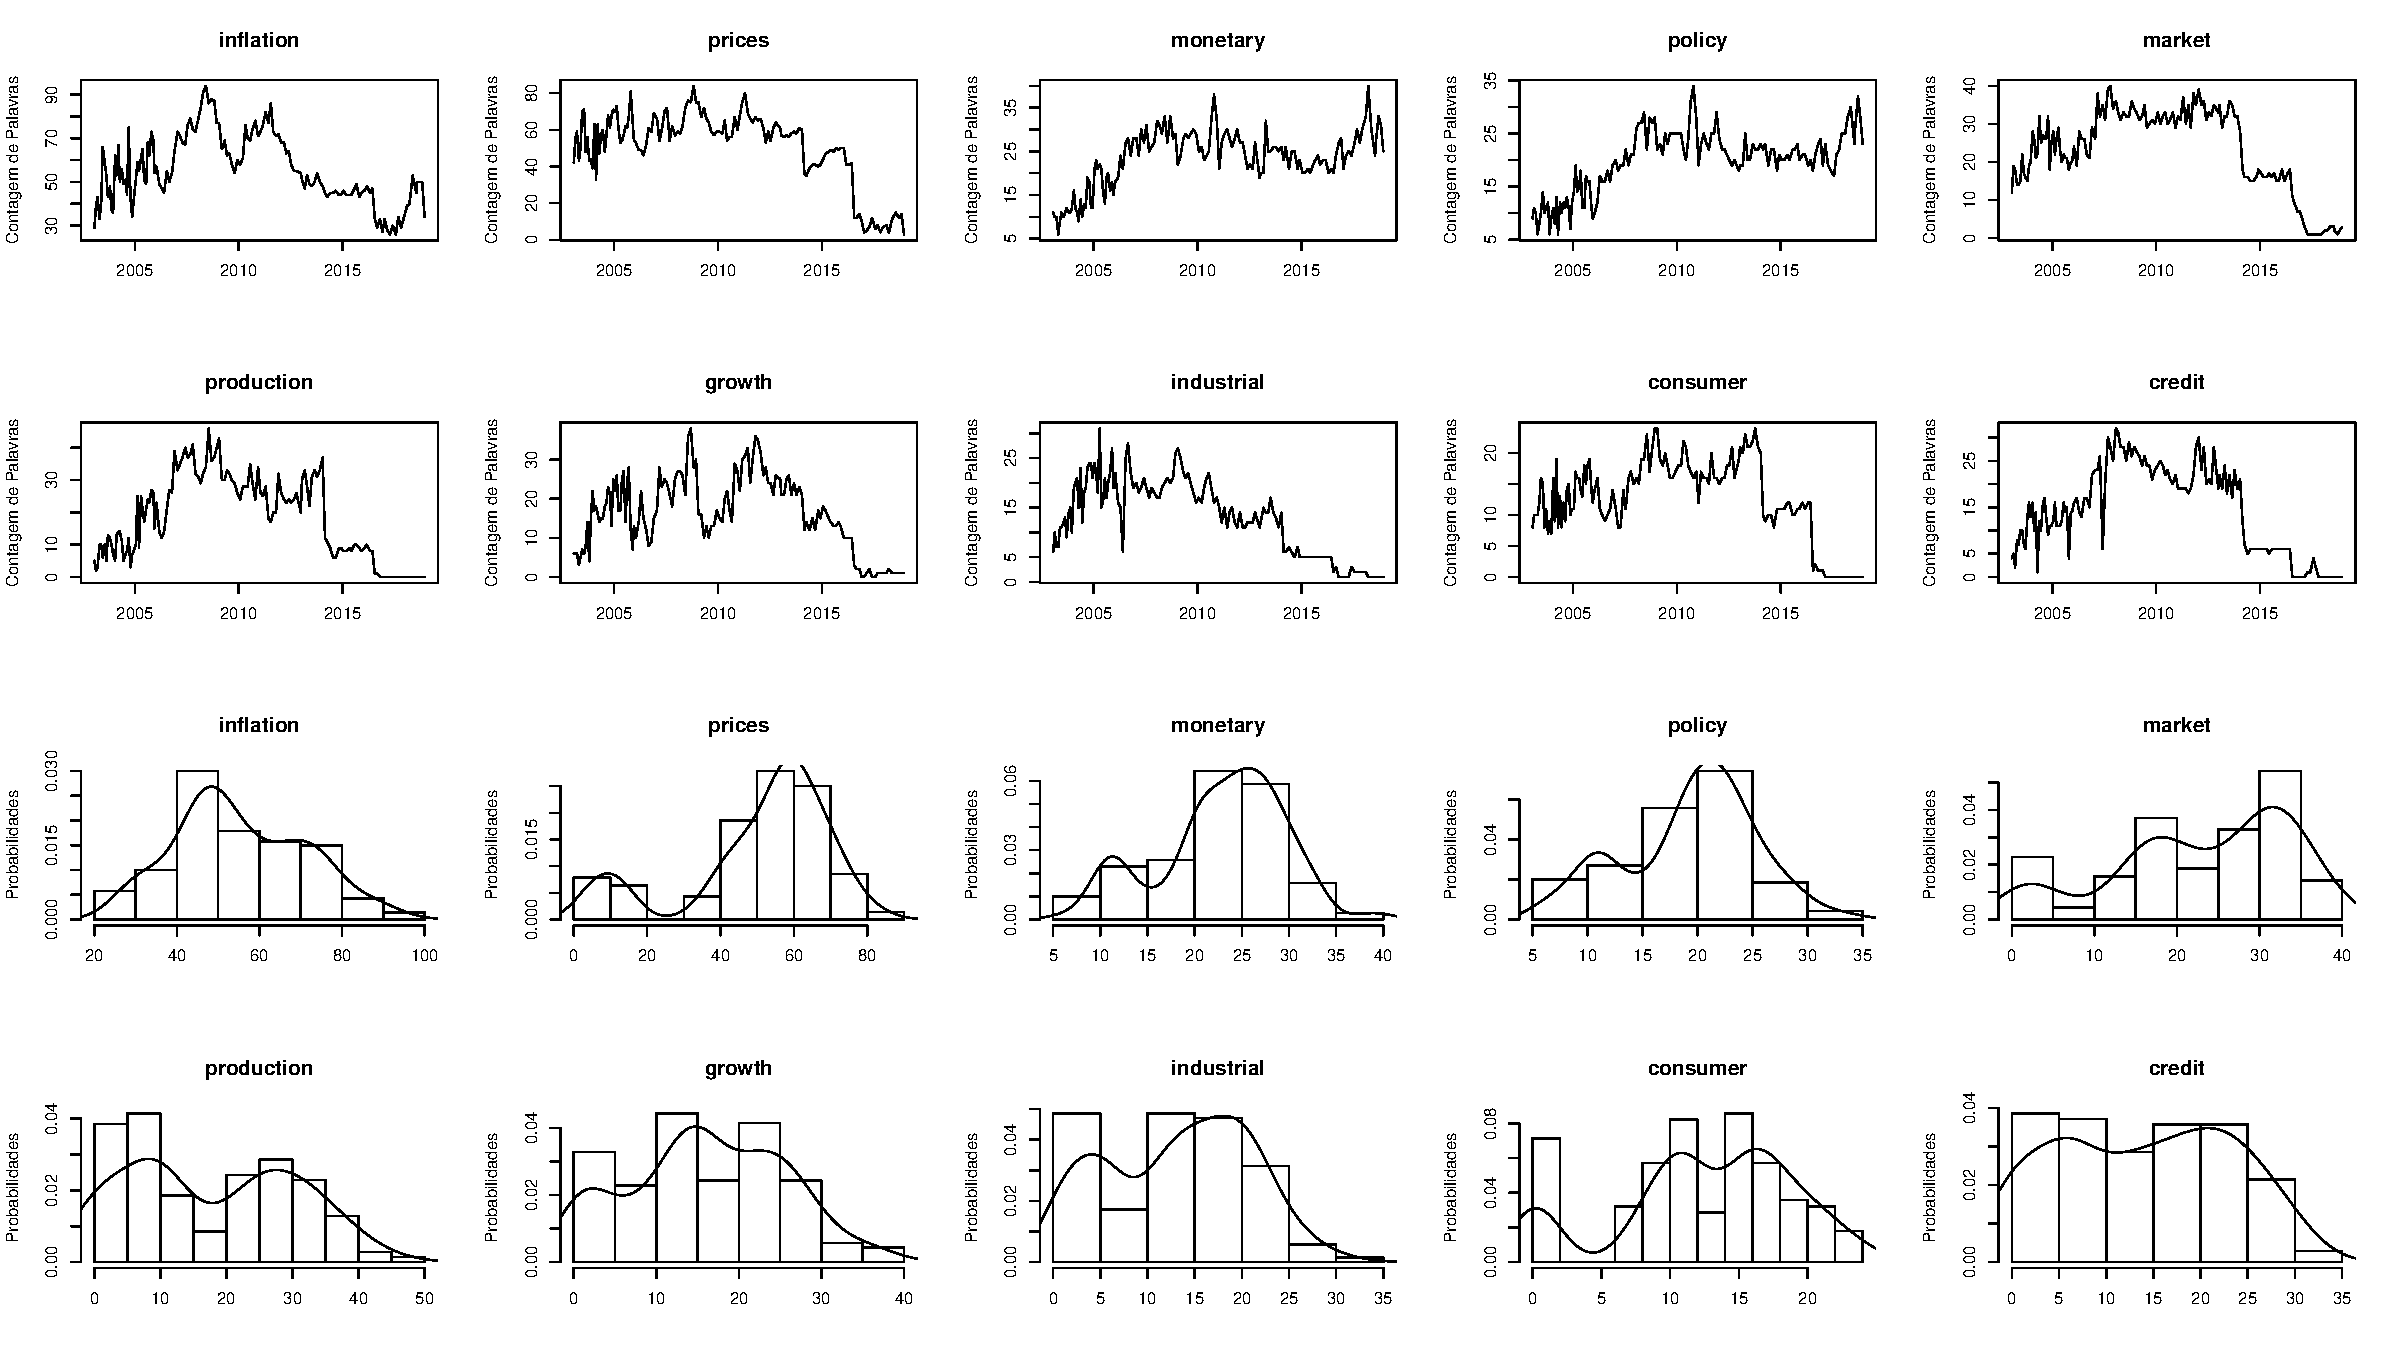
\includegraphics[width=1.5\textwidth]{capitulos/figures/analiseeconomicageral.pdf}
    \caption{Ocorrência das palavras de cunho econômico que mais aparecem (2003-2018)}
    \label{fig:analiseeconomicageral}
\end{figure}
\end{landscape}

\begin{landscape}
\begin{figure}
    \centering
    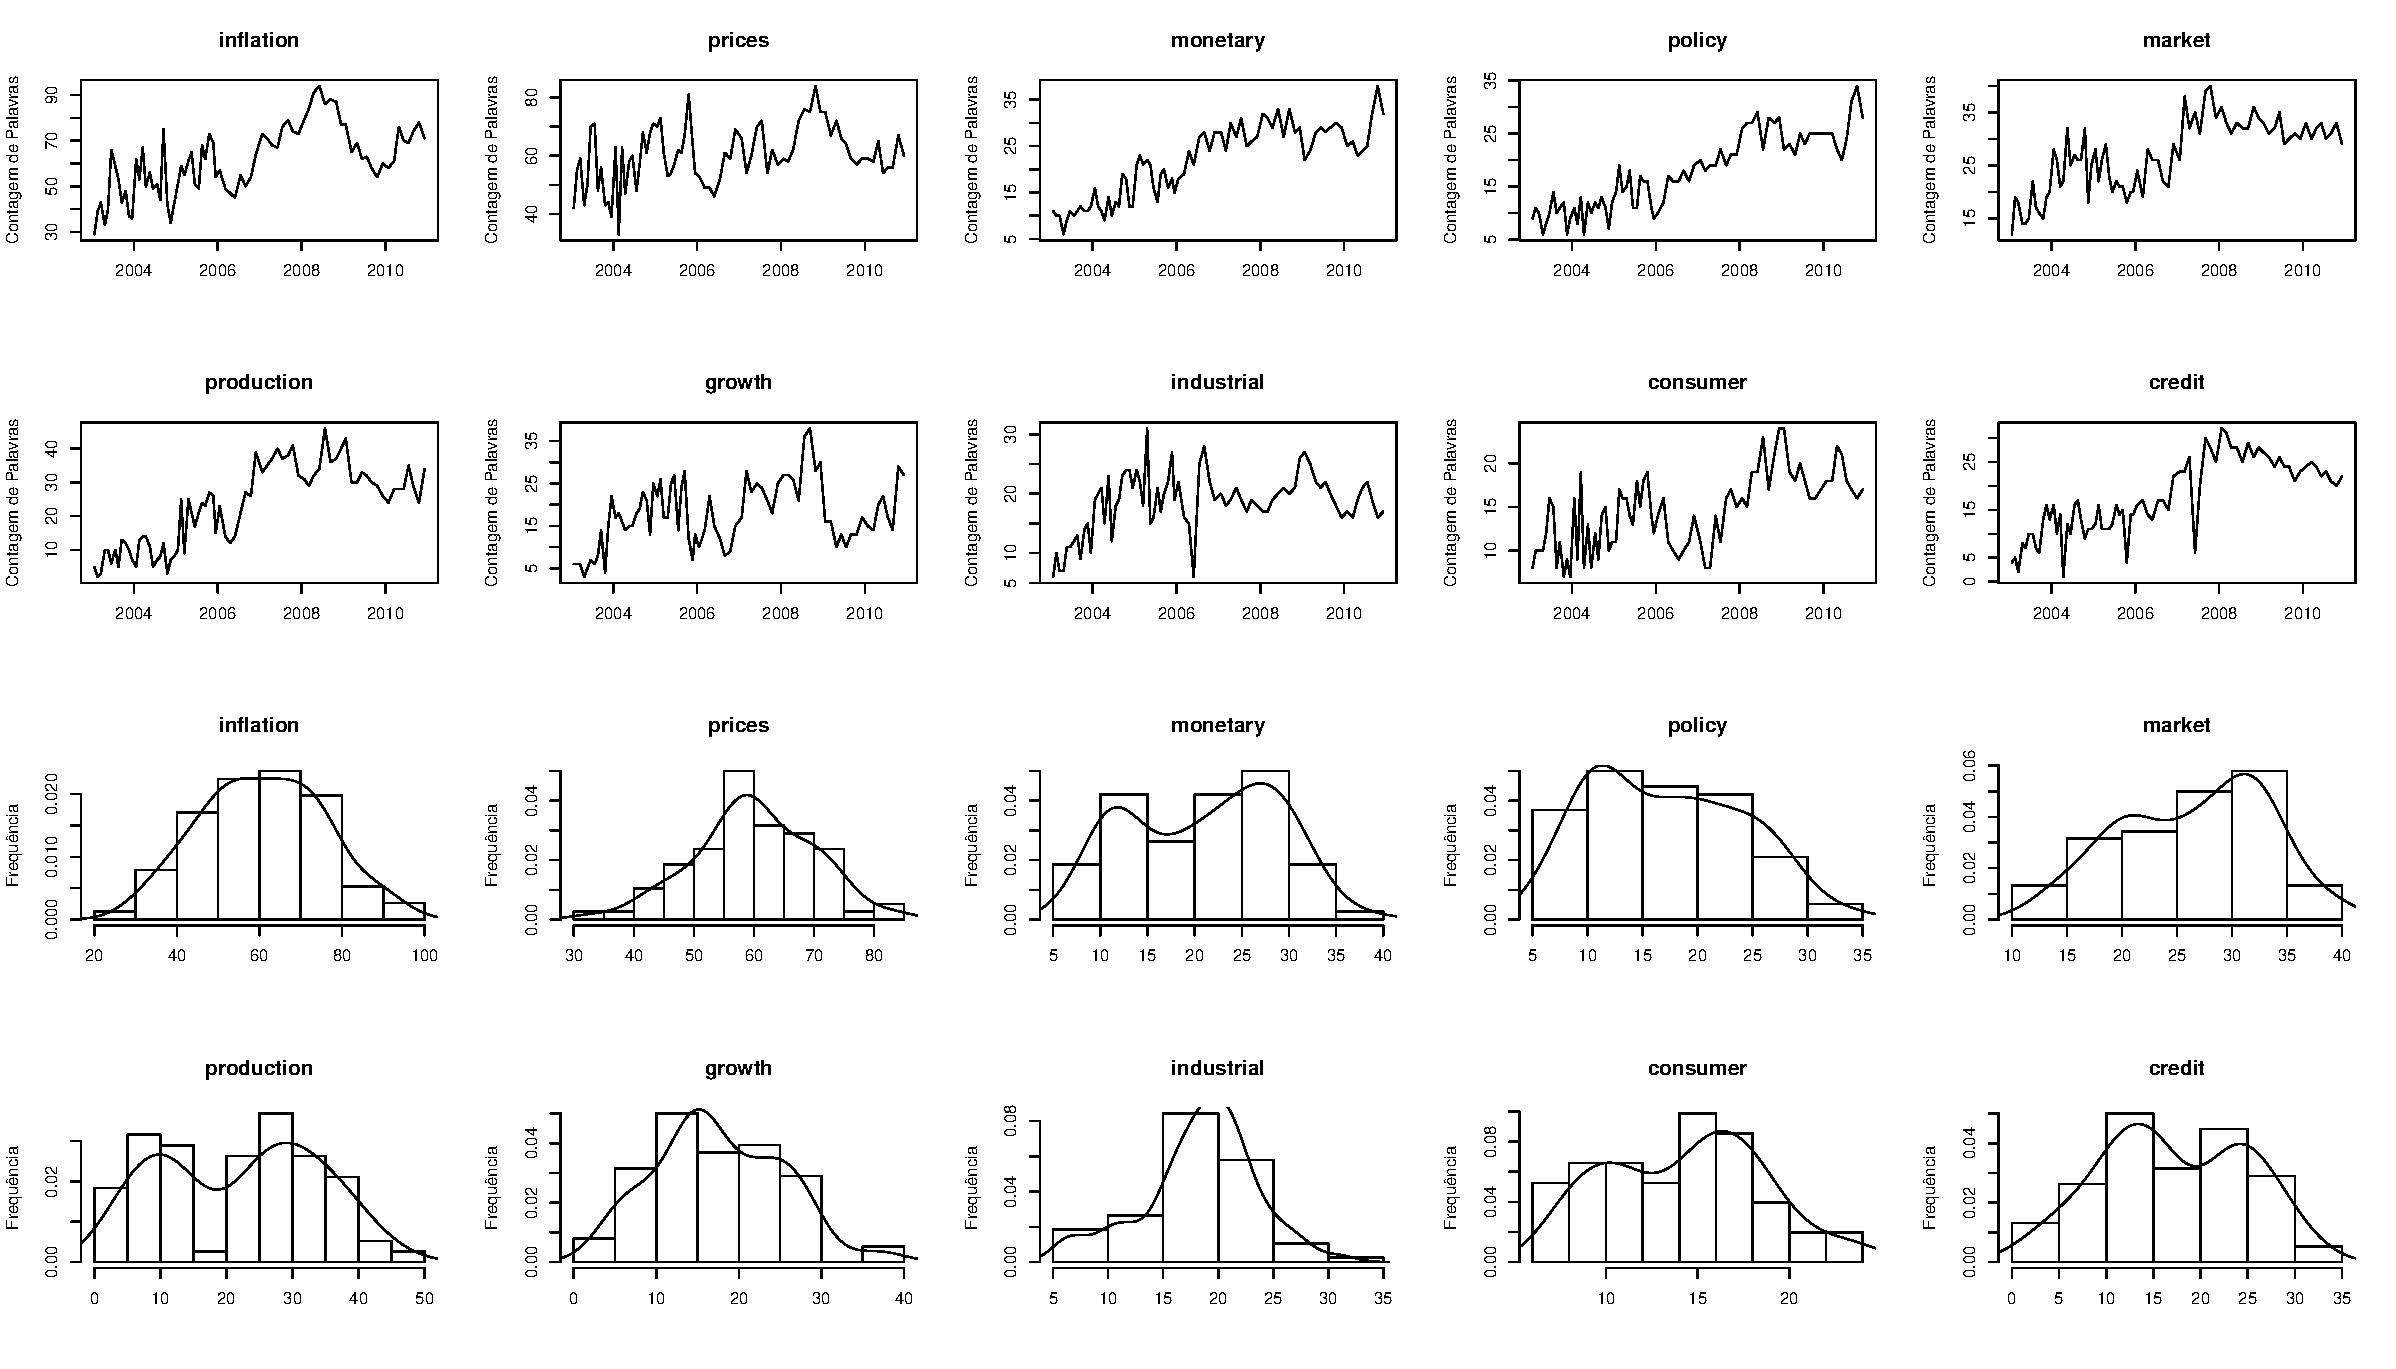
\includegraphics[width=1.5\textwidth]{capitulos/figures/analiseeconomicameirelles.pdf}
    \caption{Ocorrência das palavras de cunho econômico que mais aparecem (Gestão Meirelles)}
    \label{fig:analiseeconomicameirelles}
\end{figure}
\end{landscape}

\begin{landscape}
\begin{figure}
    \centering
    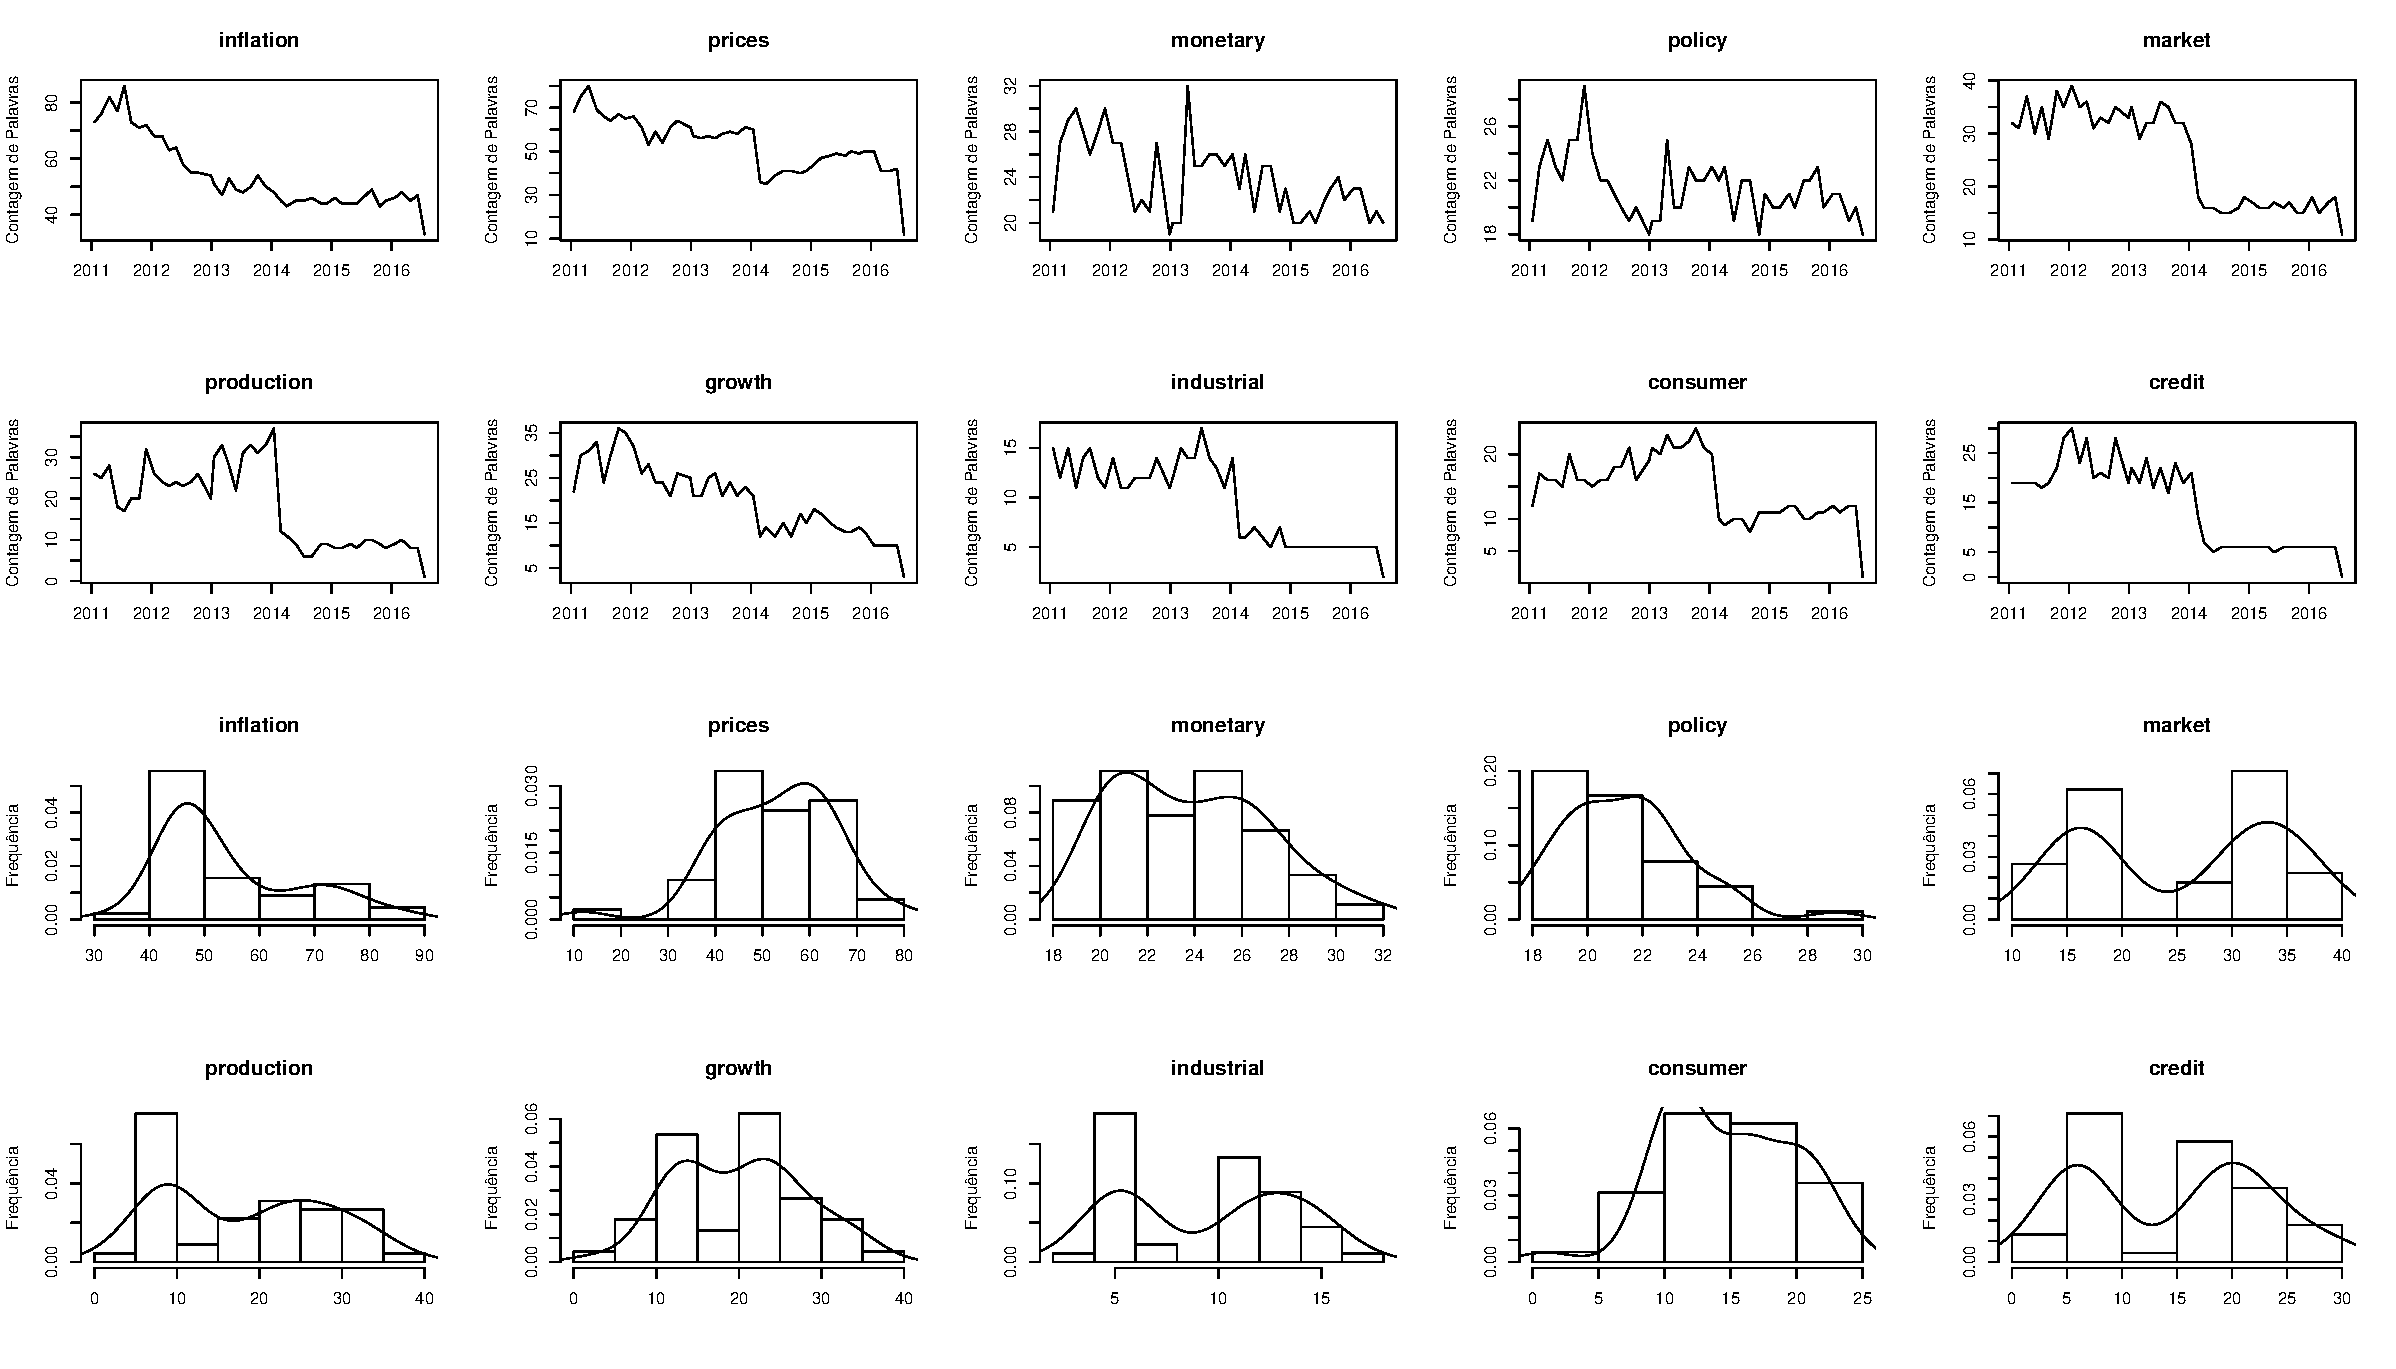
\includegraphics[width=1.5\textwidth]{capitulos/figures/analiseeconomicatombini.pdf}
    \caption{Ocorrência das palavras de cunho econômico que mais aparecem (Gestão Tombini)}
    \label{fig:analiseeconomicatombini}
\end{figure}
\end{landscape}

\begin{landscape}
\begin{figure}
    \centering
    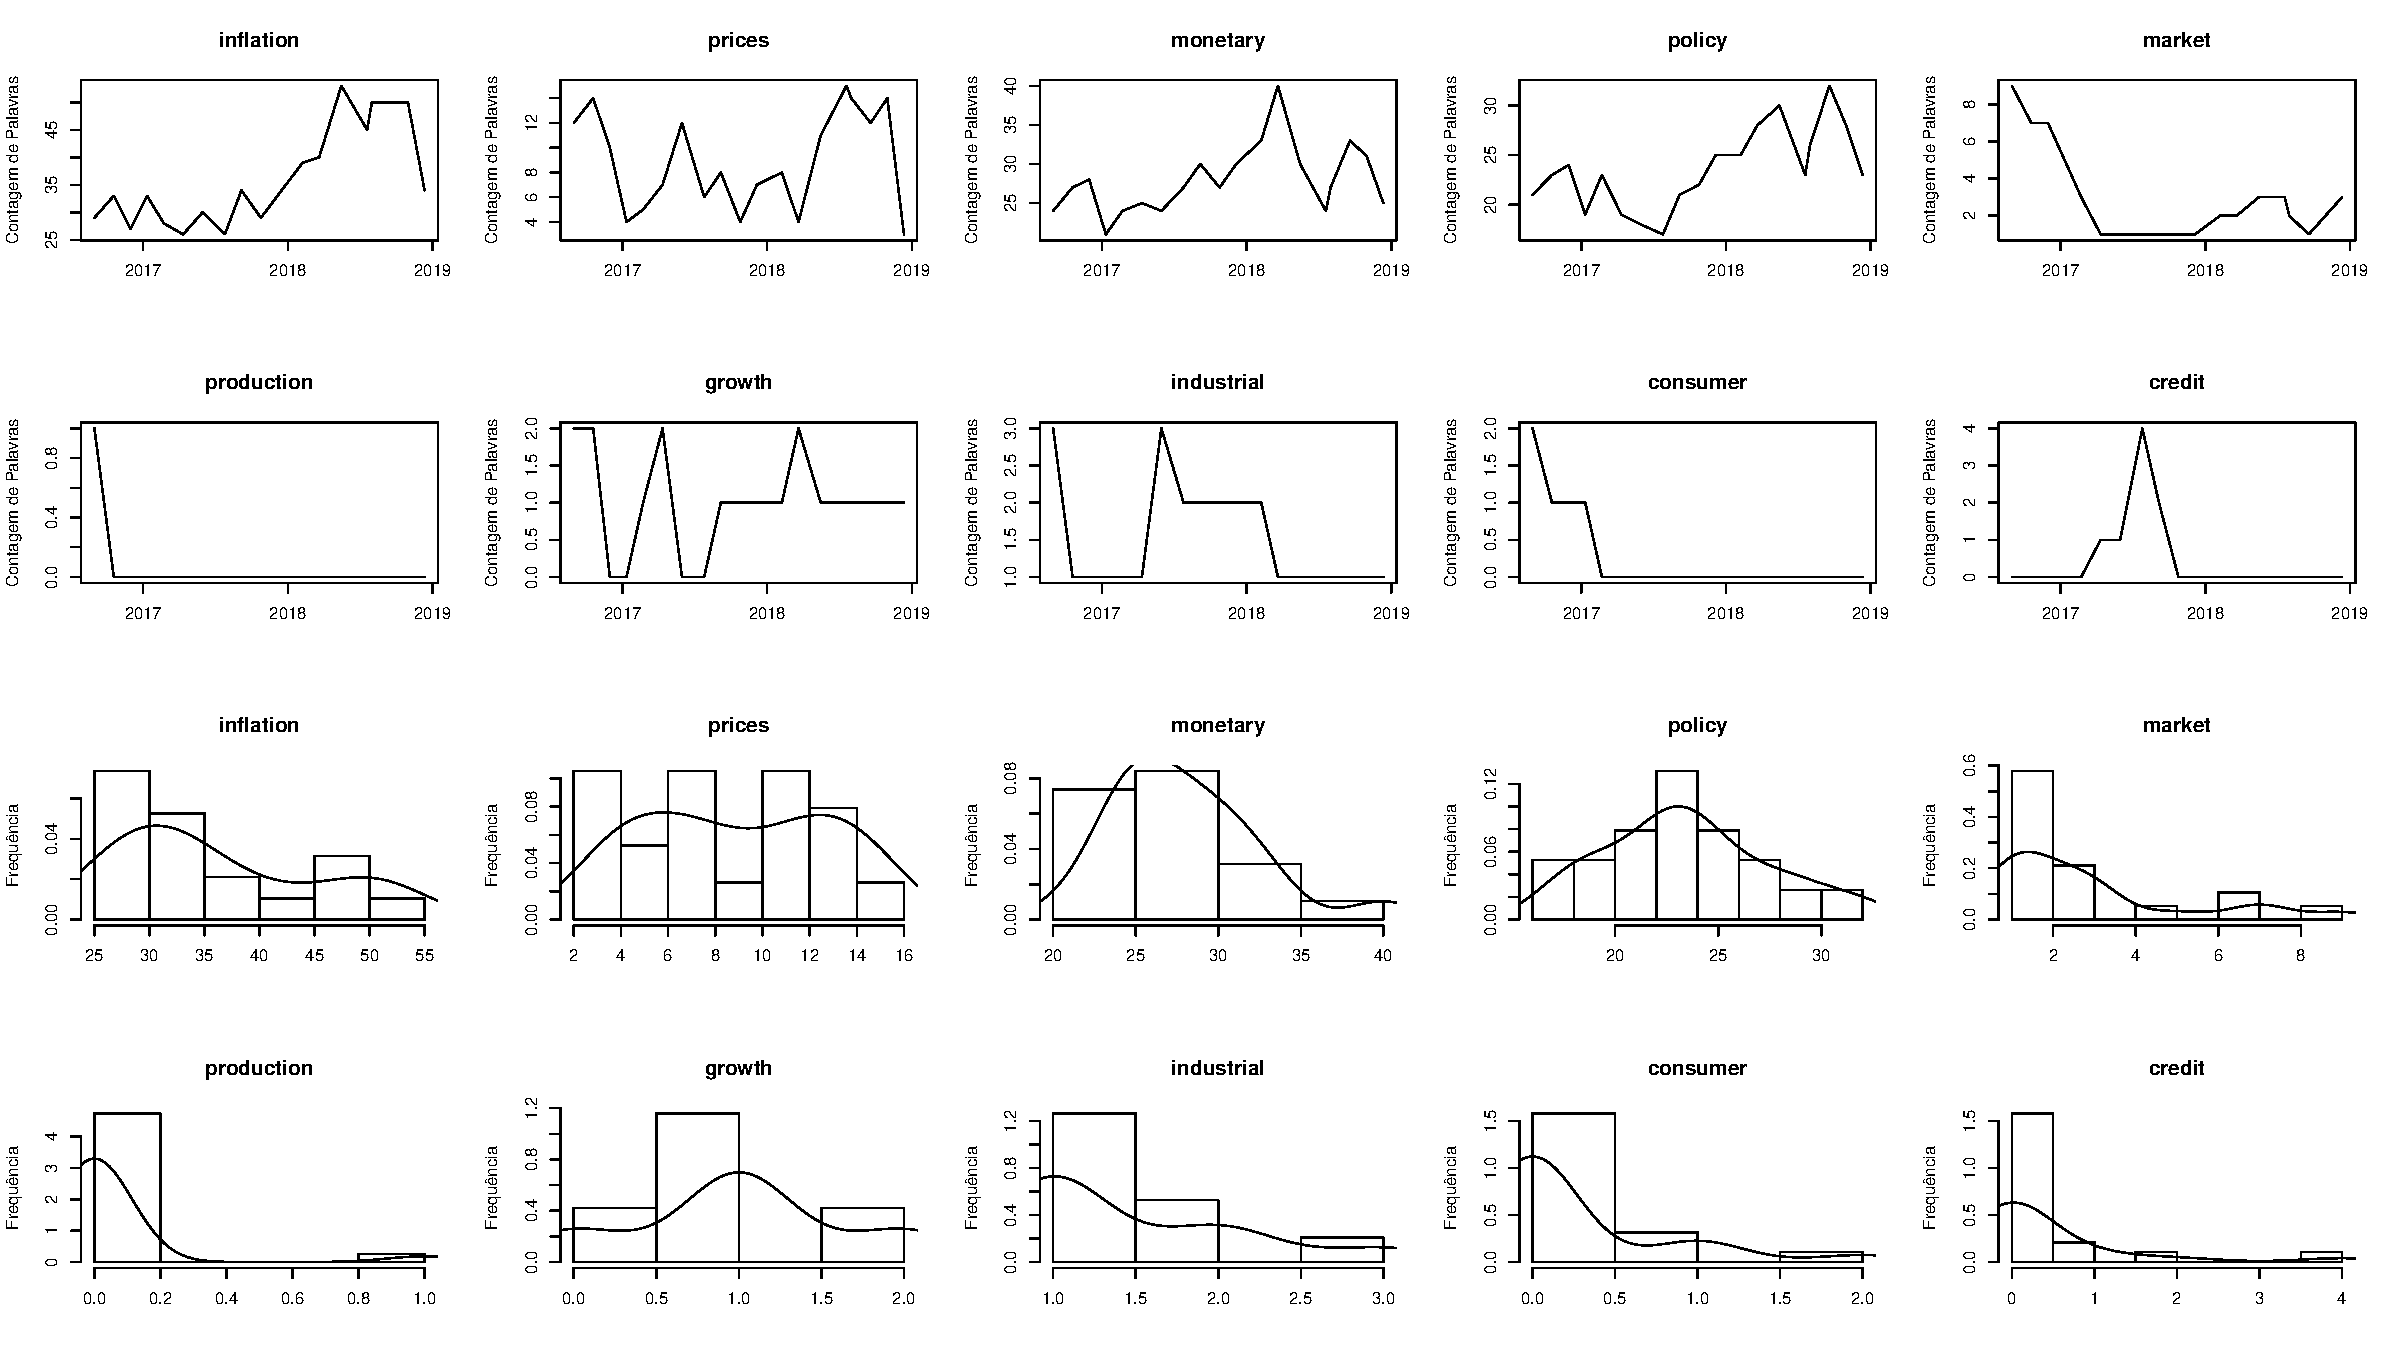
\includegraphics[width=1.5\textwidth]{capitulos/figures/analiseeconomicagoldfajn.pdf}
    \caption{Ocorrência das palavras de cunho econômico que mais aparecem (Gestão Goldfajn)}
    \label{fig:analiseeconomicagoldfajn}
\end{figure}
\end{landscape}
%\begin{landscape}
\chapter{Frequência relativa de palavras de cunho econômico e distribuição das palavras} \label{anexoa}

\begin{longtable}{rrrrrrrrrrr}
\caption{Frequência relativa de palavras de cunho econômico} \label{tab:long} \\
\hline
& inflation & prices & monetary & policy & market & production & growth & industrial & consumer & credit \\ \hline
\endfirsthead
 
\hline
& inflation & prices & monetary & policy & market & production & growth & industrial & consumer & credit \\ \hline
\endhead

\hline \multicolumn{11}{r}{{Continua na próxima página}} \\ \hline
\endfoot

\hline
\endlastfoot


ATA 80 & 0.0137 & 0.0198 & 0.0052 & 0.0042 & 0.0057 & 0.0024 & 0.0028 & 0.0028 & 0.0038 & 0.0019 \\ 
  ATA 81 & 0.0172 & 0.0243 & 0.0044 & 0.0049 & 0.0084 & 9e-04 & 0.0026 & 0.0044 & 0.0044 & 0.0022 \\ 
  ATA 82 & 0.0195 & 0.0267 & 0.0045 & 0.0045 & 0.0082 & 0.0014 & 0.0027 & 0.0032 & 0.0045 & 9e-04 \\ 
  ATA 83 & 0.0168 & 0.0218 & 0.003 & 0.003 & 0.0071 & 0.0051 & 0.0015 & 0.0036 & 0.0051 & 0.0041 \\ 
  ATA 84 & 0.0187 & 0.0233 & 0.0042 & 0.0037 & 0.0065 & 0.0047 & 0.0023 & 0.0051 & 0.0056 & 0.0033 \\ 
  ATA 85 & 0.026 & 0.0276 & 0.0043 & 0.0039 & 0.0059 & 0.0024 & 0.0028 & 0.0043 & 0.0063 & 0.0039 \\ 
  ATA 86 & 0.0206 & 0.0247 & 0.0035 & 0.0049 & 0.0077 & 0.0035 & 0.0021 & 0.0042 & 0.0052 & 0.0035 \\ 
  ATA 87 & 0.02 & 0.0182 & 0.0042 & 0.0038 & 0.0064 & 0.0019 & 0.003 & 0.0049 & 0.003 & 0.0026 \\ 
  ATA 88 & 0.0145 & 0.0188 & 0.004 & 0.0037 & 0.0054 & 0.0044 & 0.0047 & 0.003 & 0.0037 & 0.002 \\ 
  ATA 89 & 0.0178 & 0.0159 & 0.0041 & 0.0044 & 0.0056 & 0.0044 & 0.0015 & 0.0052 & 0.0026 & 0.0048 \\ 
  ATA 90 & 0.0129 & 0.0153 & 0.0038 & 0.0021 & 0.0066 & 0.0035 & 0.0052 & 0.0052 & 0.0031 & 0.0056 \\ 
  ATA 91 & 0.0135 & 0.0146 & 0.0045 & 0.0034 & 0.0075 & 0.0026 & 0.0083 & 0.0038 & 0.0026 & 0.0049 \\ 
  ATA 92 & 0.0209 & 0.0212 & 0.0054 & 0.0037 & 0.0094 & 0.0017 & 0.0057 & 0.0064 & 0.0054 & 0.0054 \\ 
  ATA 93 & 0.0196 & 0.0122 & 0.0044 & 0.003 & 0.0096 & 0.0048 & 0.0067 & 0.0074 & 0.0033 & 0.0037 \\ 
  ATA 94 & 0.0206 & 0.0194 & 0.0034 & 0.004 & 0.0065 & 0.0043 & 0.0049 & 0.0065 & 0.0058 & 0.0043 \\ 
  ATA 95 & 0.0195 & 0.0183 & 0.0035 & 0.0023 & 0.0086 & 0.0055 & 0.0055 & 0.0059 & 0.0031 & 4e-04 \\ 
  ATA 96 & 0.0182 & 0.0189 & 0.0046 & 0.0039 & 0.0104 & 0.0036 & 0.0049 & 0.0075 & 0.0042 & 0.0039 \\ 
  ATA 97 & 0.0191 & 0.0234 & 0.0039 & 0.0039 & 0.0097 & 0.0019 & 0.0058 & 0.0047 & 0.0031 & 0.0039 \\ 
  ATA 98 & 0.0178 & 0.0167 & 0.0045 & 0.0042 & 0.0094 & 0.0024 & 0.0063 & 0.0063 & 0.0042 & 0.0056 \\ 
  ATA 99 & 0.0143 & 0.0185 & 0.0039 & 0.0036 & 0.0084 & 0.0026 & 0.0062 & 0.0062 & 0.0029 & 0.0055 \\ 
  ATA 100 & 0.0202 & 0.0183 & 0.0051 & 0.0035 & 0.007 & 0.0032 & 0.0062 & 0.0062 & 0.0038 & 0.0035 \\ 
  ATA 101 & 0.0138 & 0.02 & 0.0059 & 0.0036 & 0.0105 & 0.001 & 0.0069 & 0.0079 & 0.0049 & 0.003 \\ 
  ATA 102 & 0.0117 & 0.0233 & 0.0041 & 0.0024 & 0.0062 & 0.0024 & 0.0045 & 0.0082 & 0.0034 & 0.0038 \\ 
  ATA 103 & 0.0126 & 0.0212 & 0.0036 & 0.0036 & 0.0075 & 0.0024 & 0.0075 & 0.0063 & 0.0033 & 0.0033 \\ 
  ATA 104 & 0.016 & 0.022 & 0.0066 & 0.0044 & 0.0088 & 0.0031 & 0.0069 & 0.0075 & 0.0035 & 0.0038 \\ 
  ATA 105 & 0.0169 & 0.021 & 0.0066 & 0.0055 & 0.0063 & 0.0072 & 0.0075 & 0.0063 & 0.0049 & 0.0046 \\ 
  ATA 106 & 0.0174 & 0.0193 & 0.0066 & 0.0044 & 0.0082 & 0.0028 & 0.0054 & 0.0057 & 0.0051 & 0.0035 \\ 
  ATA 107 & 0.0176 & 0.0153 & 0.0063 & 0.0043 & 0.0084 & 0.0072 & 0.0049 & 0.0089 & 0.0046 & 0.0032 \\ 
  ATA 108 & 0.0194 & 0.0161 & 0.0063 & 0.0054 & 0.0069 & 0.0063 & 0.0075 & 0.0045 & 0.0042 & 0.0033 \\ 
  ATA 109 & 0.0164 & 0.0183 & 0.0051 & 0.0035 & 0.0064 & 0.0055 & 0.0087 & 0.0051 & 0.0042 & 0.0039 \\ 
  ATA 110 & 0.0161 & 0.0204 & 0.0043 & 0.0036 & 0.0072 & 0.0069 & 0.0046 & 0.0069 & 0.0059 & 0.0053 \\ 
  ATA 111 & 0.0203 & 0.0182 & 0.0057 & 0.0051 & 0.0063 & 0.0072 & 0.0072 & 0.0051 & 0.0045 & 0.0042 \\ 
  ATA 112 & 0.0177 & 0.0191 & 0.0057 & 0.0046 & 0.006 & 0.0065 & 0.008 & 0.0057 & 0.0051 & 0.0043 \\ 
  ATA 113 & 0.021 & 0.0233 & 0.0046 & 0.0046 & 0.0052 & 0.0078 & 0.0035 & 0.0063 & 0.0055 & 0.0012 \\ 
  ATA 114 & 0.0207 & 0.0192 & 0.0054 & 0.0033 & 0.006 & 0.0078 & 0.0021 & 0.0081 & 0.0042 & 0.0042 \\ 
  ATA 115 & 0.0165 & 0.0165 & 0.0046 & 0.0027 & 0.0061 & 0.0046 & 0.004 & 0.0058 & 0.0037 & 0.0043 \\ 
  ATA 116 & 0.0176 & 0.0163 & 0.0055 & 0.0031 & 0.0074 & 0.0071 & 0.0031 & 0.0068 & 0.0043 & 0.0049 \\ 
  ATA 117 & 0.0149 & 0.0149 & 0.0058 & 0.0037 & 0.0058 & 0.0043 & 0.0043 & 0.0049 & 0.0049 & 0.0052 \\ 
  ATA 118 & 0.0139 & 0.0145 & 0.0071 & 0.005 & 0.0083 & 0.0035 & 0.0065 & 0.0044 & 0.0033 & 0.0041 \\ 
  ATA 119 & 0.0131 & 0.0134 & 0.0061 & 0.0047 & 0.0076 & 0.0041 & 0.0044 & 0.0018 & 0.0029 & 0.0038 \\ 
  ATA 120 & 0.015 & 0.0142 & 0.0074 & 0.0044 & 0.0071 & 0.0057 & 0.0033 & 0.0068 & 0.0025 & 0.0046 \\ 
  ATA 121 & 0.0126 & 0.0154 & 0.0071 & 0.0045 & 0.0055 & 0.0068 & 0.002 & 0.0071 & 0.0025 & 0.0043 \\ 
  ATA 122 & 0.0138 & 0.0151 & 0.0061 & 0.0041 & 0.0054 & 0.0067 & 0.0023 & 0.0056 & 0.0028 & 0.0038 \\ 
  ATA 123 & 0.0148 & 0.0159 & 0.0065 & 0.0044 & 0.0067 & 0.009 & 0.0035 & 0.0044 & 0.0032 & 0.0051 \\ 
  ATA 124 & 0.0171 & 0.0154 & 0.0065 & 0.0047 & 0.0061 & 0.0077 & 0.004 & 0.0047 & 0.0026 & 0.0054 \\ 
  ATA 125 & 0.0154 & 0.0117 & 0.0052 & 0.0039 & 0.0082 & 0.0076 & 0.0061 & 0.0039 & 0.0017 & 0.005 \\ 
  ATA 126 & 0.015 & 0.0132 & 0.0066 & 0.0042 & 0.0071 & 0.0082 & 0.0051 & 0.0042 & 0.0018 & 0.0057 \\ 
  ATA 127 & 0.0149 & 0.0156 & 0.006 & 0.0042 & 0.0078 & 0.0089 & 0.0056 & 0.0047 & 0.0031 & 0.0013 \\ 
  ATA 128 & 0.016 & 0.0152 & 0.0065 & 0.0046 & 0.0065 & 0.0078 & 0.0051 & 0.004 & 0.0023 & 0.0042 \\ 
  ATA 129 & 0.0178 & 0.0122 & 0.0056 & 0.0043 & 0.0088 & 0.0086 & 0.0047 & 0.0038 & 0.0036 & 0.0068 \\ 
  ATA 130 & 0.0159 & 0.0134 & 0.0056 & 0.0045 & 0.0086 & 0.0088 & 0.0039 & 0.0041 & 0.0037 & 0.006 \\ 
  ATA 131 & 0.0161 & 0.0126 & 0.0059 & 0.0046 & 0.0075 & 0.0071 & 0.0055 & 0.004 & 0.0033 & 0.0055 \\ 
  ATA 132 & 0.0169 & 0.0126 & 0.0068 & 0.0056 & 0.0077 & 0.0066 & 0.0058 & 0.0036 & 0.0034 & 0.0068 \\ 
  ATA 133 & 0.0177 & 0.0122 & 0.0065 & 0.0057 & 0.007 & 0.0061 & 0.0057 & 0.0036 & 0.0032 & 0.0065 \\ 
  ATA 134 & 0.0184 & 0.0125 & 0.0059 & 0.0055 & 0.0063 & 0.0065 & 0.0052 & 0.0038 & 0.0038 & 0.0057 \\ 
  ATA 135 & 0.0194 & 0.0149 & 0.0068 & 0.006 & 0.0068 & 0.007 & 0.0043 & 0.0041 & 0.0039 & 0.0058 \\ 
  ATA 136 & 0.0173 & 0.0153 & 0.0054 & 0.0044 & 0.0064 & 0.0092 & 0.0072 & 0.0042 & 0.0046 & 0.005 \\ 
  ATA 137 & 0.0173 & 0.0147 & 0.0065 & 0.0055 & 0.0063 & 0.0071 & 0.0075 & 0.0039 & 0.0033 & 0.0057 \\ 
  ATA 138 & 0.0163 & 0.0157 & 0.0052 & 0.0051 & 0.0067 & 0.0069 & 0.0052 & 0.0039 & 0.0039 & 0.0049 \\ 
  ATA 139 & 0.0141 & 0.0137 & 0.0053 & 0.0051 & 0.0062 & 0.0073 & 0.0055 & 0.0047 & 0.0044 & 0.0051 \\ 
  ATA 140 & 0.0144 & 0.014 & 0.0041 & 0.0041 & 0.0062 & 0.008 & 0.003 & 0.0051 & 0.0045 & 0.0051 \\ 
  ATA 141 & 0.0124 & 0.0128 & 0.0046 & 0.0044 & 0.0059 & 0.0057 & 0.0031 & 0.0048 & 0.0036 & 0.005 \\ 
  ATA 142 & 0.0144 & 0.015 & 0.0058 & 0.0044 & 0.0067 & 0.0063 & 0.0021 & 0.0046 & 0.0038 & 0.005 \\ 
  ATA 143 & 0.0121 & 0.0129 & 0.0057 & 0.0049 & 0.0069 & 0.0065 & 0.0025 & 0.0041 & 0.0039 & 0.0051 \\ 
  ATA 144 & 0.0127 & 0.0129 & 0.0056 & 0.0046 & 0.0058 & 0.0064 & 0.002 & 0.0044 & 0.0036 & 0.0048 \\ 
  ATA 145 & 0.0122 & 0.0124 & 0.0061 & 0.0053 & 0.0063 & 0.0063 & 0.0027 & 0.0042 & 0.0034 & 0.005 \\ 
  ATA 146 & 0.0114 & 0.012 & 0.0063 & 0.0053 & 0.0065 & 0.0061 & 0.0027 & 0.0038 & 0.0034 & 0.0044 \\ 
  ATA 147 & 0.013 & 0.0127 & 0.0063 & 0.0054 & 0.0065 & 0.0056 & 0.0037 & 0.0035 & 0.0037 & 0.005 \\ 
  ATA 148 & 0.0143 & 0.0146 & 0.0062 & 0.0062 & 0.0081 & 0.0059 & 0.0037 & 0.0042 & 0.0044 & 0.0059 \\ 
  ATA 149 & 0.0134 & 0.0127 & 0.0057 & 0.0055 & 0.0066 & 0.0062 & 0.0031 & 0.0035 & 0.004 & 0.0055 \\ 
  ATA 150 & 0.0162 & 0.0138 & 0.0049 & 0.0047 & 0.0068 & 0.006 & 0.0043 & 0.004 & 0.0047 & 0.0051 \\ 
  ATA 151 & 0.0153 & 0.0118 & 0.0052 & 0.0044 & 0.0072 & 0.0061 & 0.0048 & 0.0046 & 0.0046 & 0.0048 \\ 
  ATA 152 & 0.0156 & 0.0127 & 0.0057 & 0.0054 & 0.0068 & 0.0079 & 0.0039 & 0.005 & 0.0041 & 0.0052 \\ 
  ATA 153 & 0.0163 & 0.0123 & 0.007 & 0.0068 & 0.0068 & 0.0064 & 0.0031 & 0.0042 & 0.0037 & 0.0046 \\ 
  ATA 154 & 0.0155 & 0.0133 & 0.0076 & 0.0068 & 0.0066 & 0.0048 & 0.0058 & 0.0032 & 0.0032 & 0.004 \\ 
  ATA 155 & 0.0145 & 0.0123 & 0.0065 & 0.0057 & 0.0059 & 0.0069 & 0.0055 & 0.0035 & 0.0035 & 0.0045 \\ 
  ATA 156 & 0.0157 & 0.0146 & 0.0045 & 0.0041 & 0.0069 & 0.0056 & 0.0047 & 0.0032 & 0.0026 & 0.0041 \\ 
  ATA 157 & 0.0158 & 0.0156 & 0.0056 & 0.0048 & 0.0065 & 0.0052 & 0.0063 & 0.0025 & 0.0035 & 0.004 \\ 
  ATA 158 & 0.0154 & 0.015 & 0.0054 & 0.0047 & 0.0069 & 0.0052 & 0.0058 & 0.0028 & 0.003 & 0.0036 \\ 
  ATA 159 & 0.0155 & 0.0139 & 0.006 & 0.0046 & 0.006 & 0.0036 & 0.0066 & 0.0022 & 0.0032 & 0.0038 \\ 
  ATA 160 & 0.0178 & 0.0136 & 0.0058 & 0.0045 & 0.0072 & 0.0035 & 0.005 & 0.0029 & 0.0031 & 0.0037 \\ 
  ATA 161 & 0.0145 & 0.0127 & 0.0052 & 0.005 & 0.0058 & 0.004 & 0.006 & 0.003 & 0.004 & 0.0038 \\ 
  ATA 162 & 0.0135 & 0.0128 & 0.0053 & 0.0048 & 0.0072 & 0.0038 & 0.0069 & 0.0023 & 0.003 & 0.0042 \\ 
  ATA 163 & 0.0137 & 0.0123 & 0.0057 & 0.0055 & 0.0066 & 0.0061 & 0.0066 & 0.0021 & 0.003 & 0.0053 \\ 
  ATA 164 & 0.0127 & 0.0123 & 0.005 & 0.0045 & 0.0073 & 0.0048 & 0.006 & 0.0026 & 0.0028 & 0.0056 \\ 
  ATA 165 & 0.0126 & 0.0113 & 0.005 & 0.0041 & 0.0065 & 0.0045 & 0.0048 & 0.002 & 0.003 & 0.0043 \\ 
  ATA 166 & 0.0121 & 0.0102 & 0.0046 & 0.0042 & 0.0069 & 0.0044 & 0.0054 & 0.0021 & 0.0031 & 0.0054 \\ 
  ATA 167 & 0.0126 & 0.0117 & 0.0041 & 0.0041 & 0.0061 & 0.0047 & 0.0047 & 0.0024 & 0.0036 & 0.0039 \\ 
  ATA 168 & 0.0116 & 0.0108 & 0.0044 & 0.004 & 0.0066 & 0.0046 & 0.0048 & 0.0024 & 0.0036 & 0.0042 \\ 
  ATA 169 & 0.0109 & 0.012 & 0.0041 & 0.0038 & 0.0063 & 0.0047 & 0.0041 & 0.0024 & 0.0041 & 0.004 \\ 
  ATA 170 & 0.0106 & 0.0124 & 0.0052 & 0.0039 & 0.0068 & 0.005 & 0.005 & 0.0027 & 0.0031 & 0.0054 \\ 
  ATA 171 & 0.0112 & 0.0127 & 0.0039 & 0.0037 & 0.0069 & 0.0042 & 0.0052 & 0.0023 & 0.0039 & 0.0039 \\ 
  ATA 172 & 0.0102 & 0.0114 & 0.004 & 0.0038 & 0.007 & 0.006 & 0.0042 & 0.0024 & 0.0042 & 0.0044 \\ 
  ATA 173 & 0.0095 & 0.0113 & 0.004 & 0.0038 & 0.0058 & 0.0066 & 0.0042 & 0.003 & 0.004 & 0.0038 \\ 
  ATA 174 & 0.011 & 0.0118 & 0.0066 & 0.0052 & 0.0066 & 0.0058 & 0.0052 & 0.0029 & 0.0048 & 0.005 \\ 
  ATA 175 & 0.0105 & 0.012 & 0.0054 & 0.0043 & 0.0069 & 0.0047 & 0.0056 & 0.003 & 0.0045 & 0.0039 \\ 
  ATA 176 & 0.0106 & 0.0128 & 0.0055 & 0.0044 & 0.008 & 0.0069 & 0.0046 & 0.0038 & 0.0046 & 0.0049 \\ 
  ATA 177 & 0.0105 & 0.0124 & 0.0055 & 0.0048 & 0.0073 & 0.0069 & 0.005 & 0.0029 & 0.0046 & 0.0036 \\ 
  ATA 178 & 0.0111 & 0.0119 & 0.0054 & 0.0045 & 0.0066 & 0.0064 & 0.0043 & 0.0027 & 0.0049 & 0.0047 \\ 
  ATA 179 & 0.0105 & 0.0128 & 0.0053 & 0.0046 & 0.0067 & 0.0069 & 0.0048 & 0.0023 & 0.0044 & 0.004 \\ 
  ATA 180 & 0.0099 & 0.0123 & 0.0053 & 0.0047 & 0.0058 & 0.0076 & 0.0043 & 0.0029 & 0.0041 & 0.0043 \\ 
  ATA 181 & 0.0199 & 0.0159 & 0.0101 & 0.0097 & 0.0079 & 0.0053 & 0.0053 & 0.0026 & 0.0044 & 0.0053 \\ 
  ATA 182 & 0.019 & 0.0155 & 0.0115 & 0.0102 & 0.0071 & 0.0049 & 0.0062 & 0.0027 & 0.004 & 0.0031 \\ 
  ATA 183 & 0.0217 & 0.0188 & 0.0101 & 0.0092 & 0.0077 & 0.0043 & 0.0058 & 0.0034 & 0.0048 & 0.0024 \\ 
  ATA 184 & 0.0205 & 0.0187 & 0.0114 & 0.01 & 0.0068 & 0.0027 & 0.0068 & 0.0027 & 0.0046 & 0.0027 \\ 
  ATA 185 & 0.021 & 0.0187 & 0.0114 & 0.01 & 0.0068 & 0.0027 & 0.0055 & 0.0023 & 0.0036 & 0.0027 \\ 
  ATA 186 & 0.0209 & 0.019 & 0.01 & 0.0085 & 0.0076 & 0.0043 & 0.0081 & 0.0033 & 0.0052 & 0.0028 \\ 
  ATA 187 & 0.0204 & 0.019 & 0.0106 & 0.0097 & 0.0083 & 0.0042 & 0.0069 & 0.0023 & 0.0051 & 0.0028 \\ 
  ATA 188 & 0.0223 & 0.0213 & 0.0097 & 0.0097 & 0.0082 & 0.0039 & 0.0087 & 0.0024 & 0.0053 & 0.0029 \\ 
  ATA 189 & 0.0211 & 0.0226 & 0.0096 & 0.0096 & 0.0077 & 0.0038 & 0.0082 & 0.0024 & 0.0053 & 0.0029 \\ 
  ATA 190 & 0.021 & 0.023 & 0.01 & 0.01 & 0.0077 & 0.0043 & 0.0072 & 0.0024 & 0.0057 & 0.0029 \\ 
  ATA 191 & 0.0206 & 0.0229 & 0.0093 & 0.0093 & 0.0079 & 0.0037 & 0.0065 & 0.0023 & 0.0056 & 0.0023 \\ 
  ATA 192 & 0.022 & 0.0225 & 0.0103 & 0.0103 & 0.0075 & 0.0047 & 0.0061 & 0.0023 & 0.0047 & 0.0028 \\ 
  ATA 193 & 0.0216 & 0.022 & 0.0101 & 0.0097 & 0.0075 & 0.0044 & 0.0057 & 0.0022 & 0.0044 & 0.0026 \\ 
  ATA 194 & 0.0201 & 0.0229 & 0.0112 & 0.0108 & 0.007 & 0.0042 & 0.0065 & 0.0023 & 0.0051 & 0.0028 \\ 
  ATA 195 & 0.0206 & 0.0229 & 0.0101 & 0.0092 & 0.0069 & 0.0037 & 0.006 & 0.0023 & 0.005 & 0.0027 \\ 
  ATA 196 & 0.0204 & 0.0222 & 0.0102 & 0.0093 & 0.008 & 0.004 & 0.0044 & 0.0022 & 0.0053 & 0.0027 \\ 
  ATA 197 & 0.0216 & 0.0185 & 0.0104 & 0.0095 & 0.0068 & 0.0045 & 0.0045 & 0.0023 & 0.005 & 0.0027 \\ 
  ATA 198 & 0.0208 & 0.019 & 0.0093 & 0.0088 & 0.0079 & 0.0037 & 0.0046 & 0.0023 & 0.0056 & 0.0028 \\ 
  ATA 199 & 0.0213 & 0.019 & 0.0095 & 0.0091 & 0.0082 & 0.0036 & 0.0045 & 0.0023 & 0.0054 & 0.0027 \\ 
  ATA 200 & 0.0292 & 0.0106 & 0.0177 & 0.0159 & 0.0097 & 9e-04 & 0.0027 & 0.0018 & 9e-04 & 0 \\ 
  ATA 201 & 0.023 & 0.0095 & 0.0191 & 0.0167 & 0.0071 & 8e-04 & 0.0016 & 0.0024 & 0.0016 & 0 \\ 
  ATA 202 & 0.0252 & 0.0107 & 0.0207 & 0.0176 & 0.0054 & 0 & 0.0015 & 8e-04 & 8e-04 & 0 \\ 
  ATA 203 & 0.0224 & 0.0083 & 0.0232 & 0.0199 & 0.0058 & 0 & 0 & 8e-04 & 8e-04 & 0 \\ 
  ATA 204 & 0.0278 & 0.0034 & 0.0177 & 0.016 & 0.0042 & 0 & 0 & 8e-04 & 8e-04 & 0 \\ 
  ATA 205 & 0.0233 & 0.0042 & 0.02 & 0.0191 & 0.0025 & 0 & 8e-04 & 8e-04 & 0 & 0 \\ 
  ATA 206 & 0.0212 & 0.0057 & 0.0204 & 0.0155 & 8e-04 & 0 & 0.0016 & 8e-04 & 0 & 8e-04 \\ 
  ATA 207 & 0.0235 & 0.0094 & 0.0188 & 0.0141 & 8e-04 & 0 & 0 & 0.0024 & 0 & 8e-04 \\ 
  ATA 208 & 0.0202 & 0.0047 & 0.021 & 0.0132 & 8e-04 & 0 & 0 & 0.0016 & 0 & 0.0031 \\ 
  ATA 209 & 0.0236 & 0.0055 & 0.0208 & 0.0146 & 7e-04 & 0 & 7e-04 & 0.0014 & 0 & 0.0014 \\ 
  ATA 210 & 0.0234 & 0.0032 & 0.0218 & 0.0178 & 8e-04 & 0 & 8e-04 & 0.0016 & 0 & 0 \\ 
  ATA 211 & 0.0248 & 0.0053 & 0.0225 & 0.0188 & 8e-04 & 0 & 8e-04 & 0.0015 & 0 & 0 \\ 
  ATA 212 & 0.0286 & 0.0059 & 0.0242 & 0.0183 & 0.0015 & 0 & 7e-04 & 0.0015 & 0 & 0 \\ 
  ATA 213 & 0.0273 & 0.0027 & 0.0273 & 0.0191 & 0.0014 & 0 & 0.0014 & 7e-04 & 0 & 0 \\ 
  ATA 214 & 0.0349 & 0.0072 & 0.0198 & 0.0198 & 0.002 & 0 & 7e-04 & 7e-04 & 0 & 0 \\ 
  ATA 215 & 0.0307 & 0.0102 & 0.0163 & 0.0157 & 0.002 & 0 & 7e-04 & 7e-04 & 0 & 0 \\ 
  ATA 216 & 0.0335 & 0.0094 & 0.0181 & 0.0174 & 0.0013 & 0 & 7e-04 & 7e-04 & 0 & 0 \\ 
  ATA 217 & 0.0337 & 0.0081 & 0.0222 & 0.0215 & 7e-04 & 0 & 7e-04 & 7e-04 & 0 & 0 \\ 
  ATA 218 & 0.0342 & 0.0096 & 0.0212 & 0.0192 & 0.0014 & 0 & 7e-04 & 7e-04 & 0 & 0 \\ 
  ATA 219 & 0.028 & 0.0025 & 0.0206 & 0.0189 & 0.0025 & 0 & 8e-04 & 8e-04 & 0 & 0 \\ 
   \hline
\end{longtable}
\end{landscape}

\begin{landscape}
\begin{figure}
    \centering
    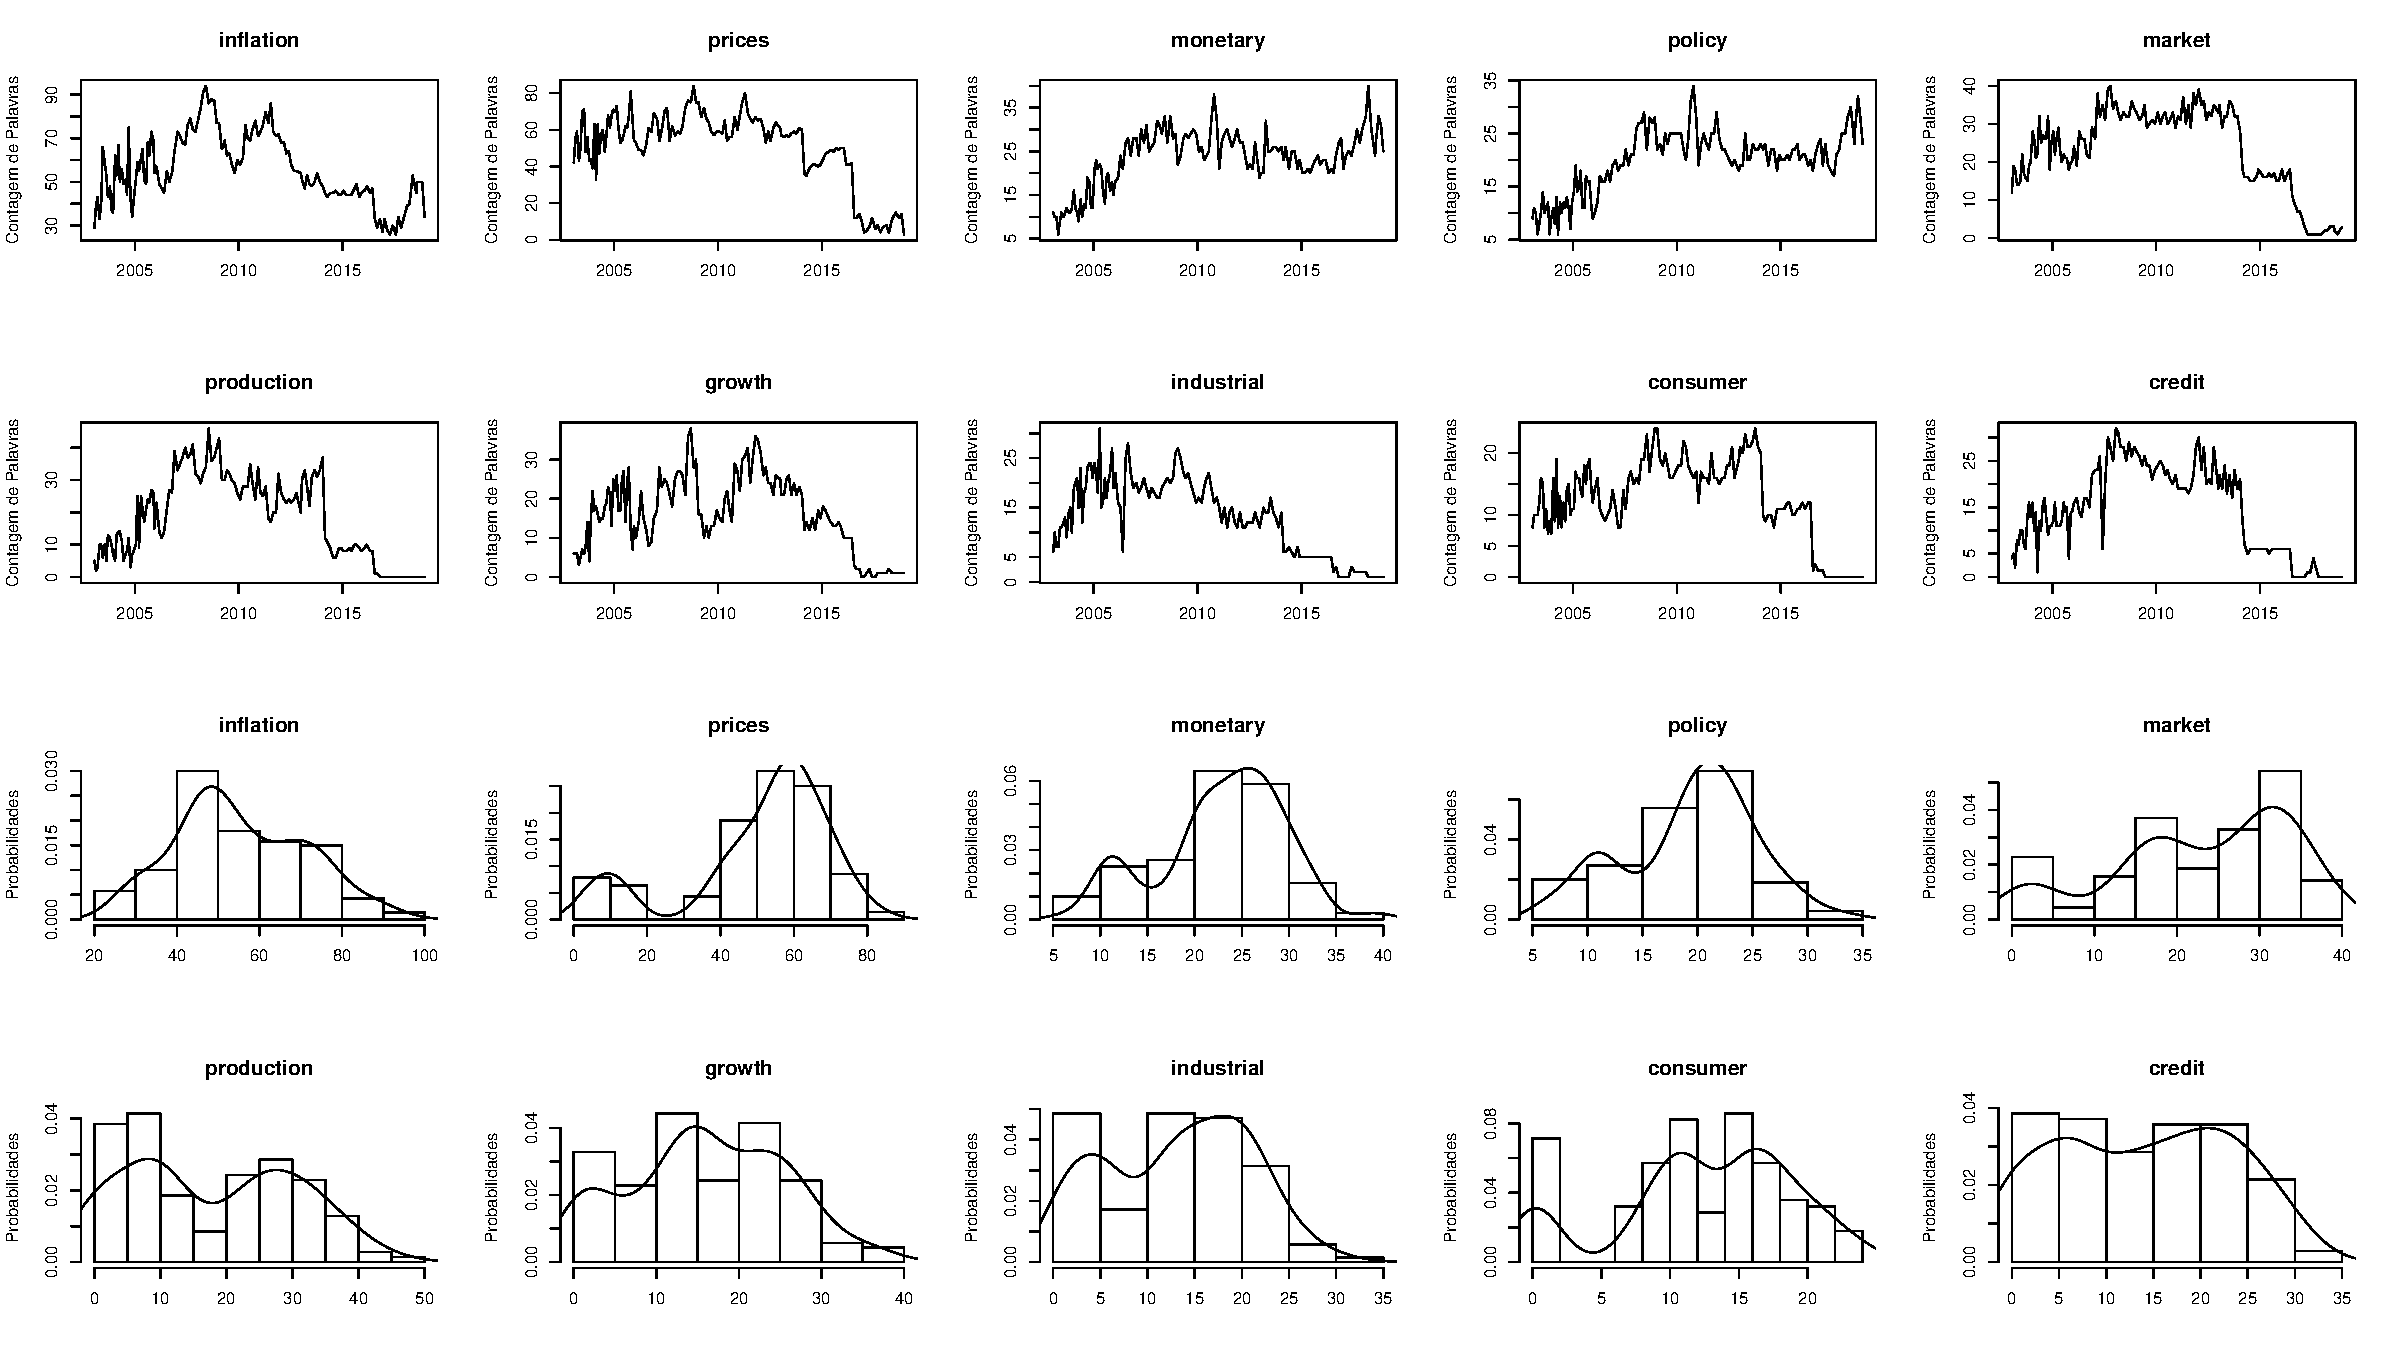
\includegraphics[width=1.5\textwidth]{capitulos/figures/analiseeconomicageral.pdf}
    \caption{Frequência relativa das palavras de cunho econômico que mais aparecem (2003-2018)}
    \label{fig:analiseeconomicageral}
\end{figure}
\end{landscape}

\begin{landscape}
\begin{figure}
    \centering
    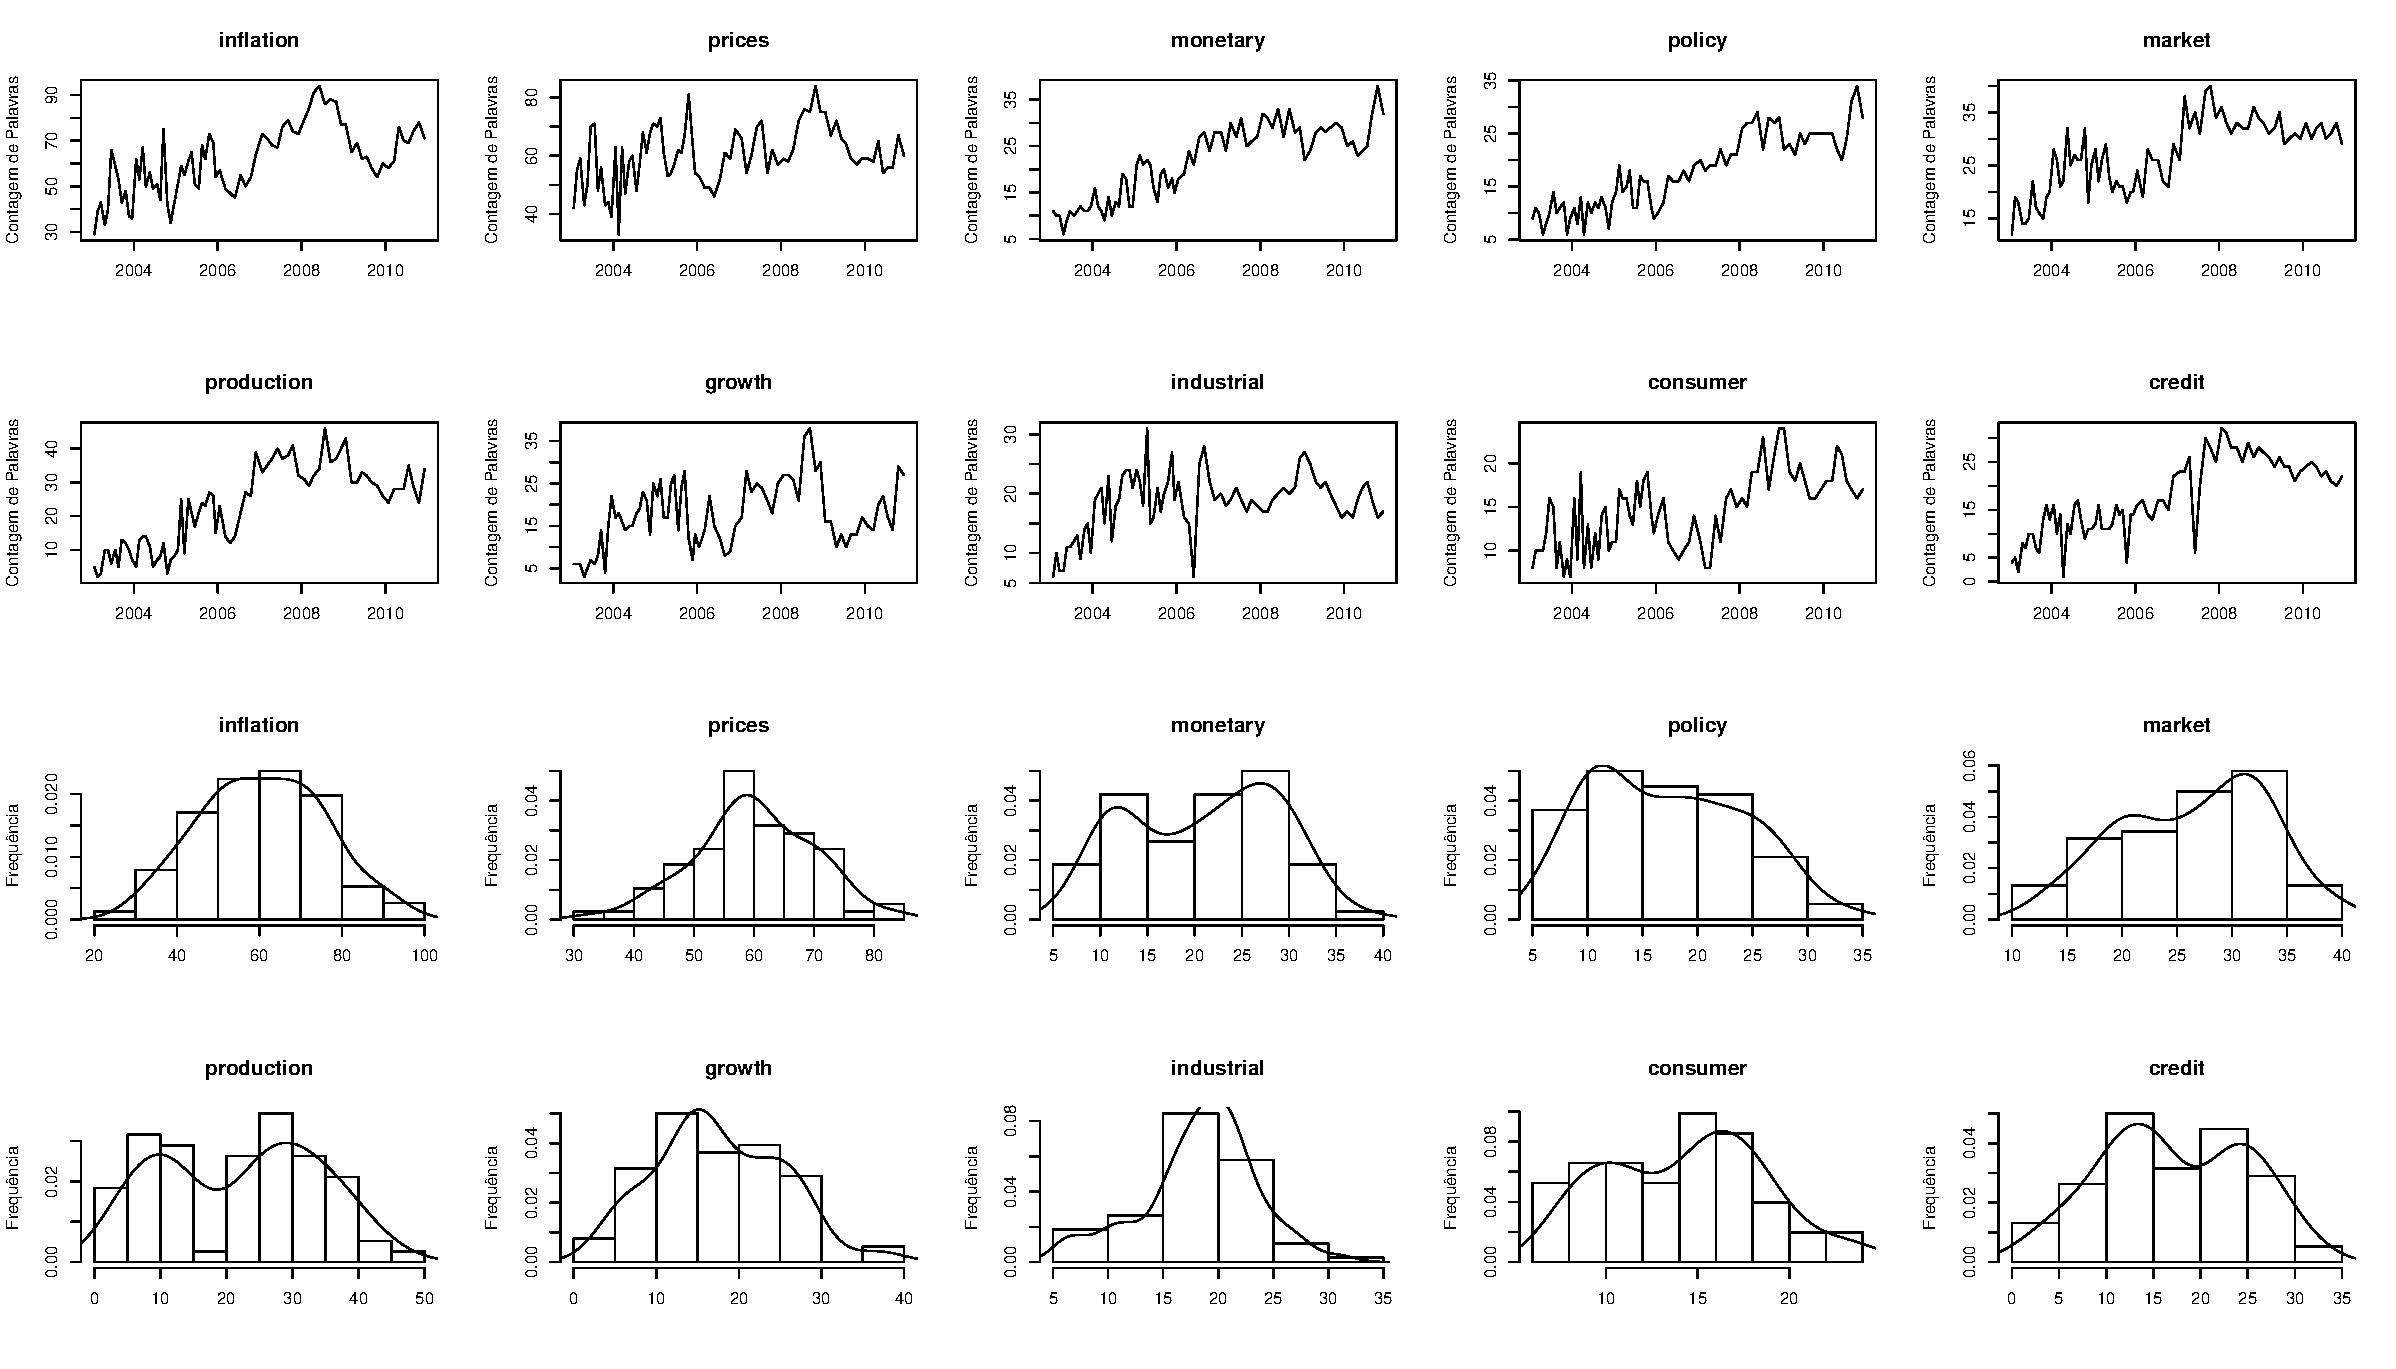
\includegraphics[width=1.5\textwidth]{capitulos/figures/analiseeconomicameirelles.pdf}
    \caption{Frequência relativa das palavras de cunho econômico que mais aparecem (Gestão Meirelles)}
    \label{fig:analiseeconomicameirelles}
\end{figure}
\end{landscape}

\begin{landscape}
\begin{figure}
    \centering
    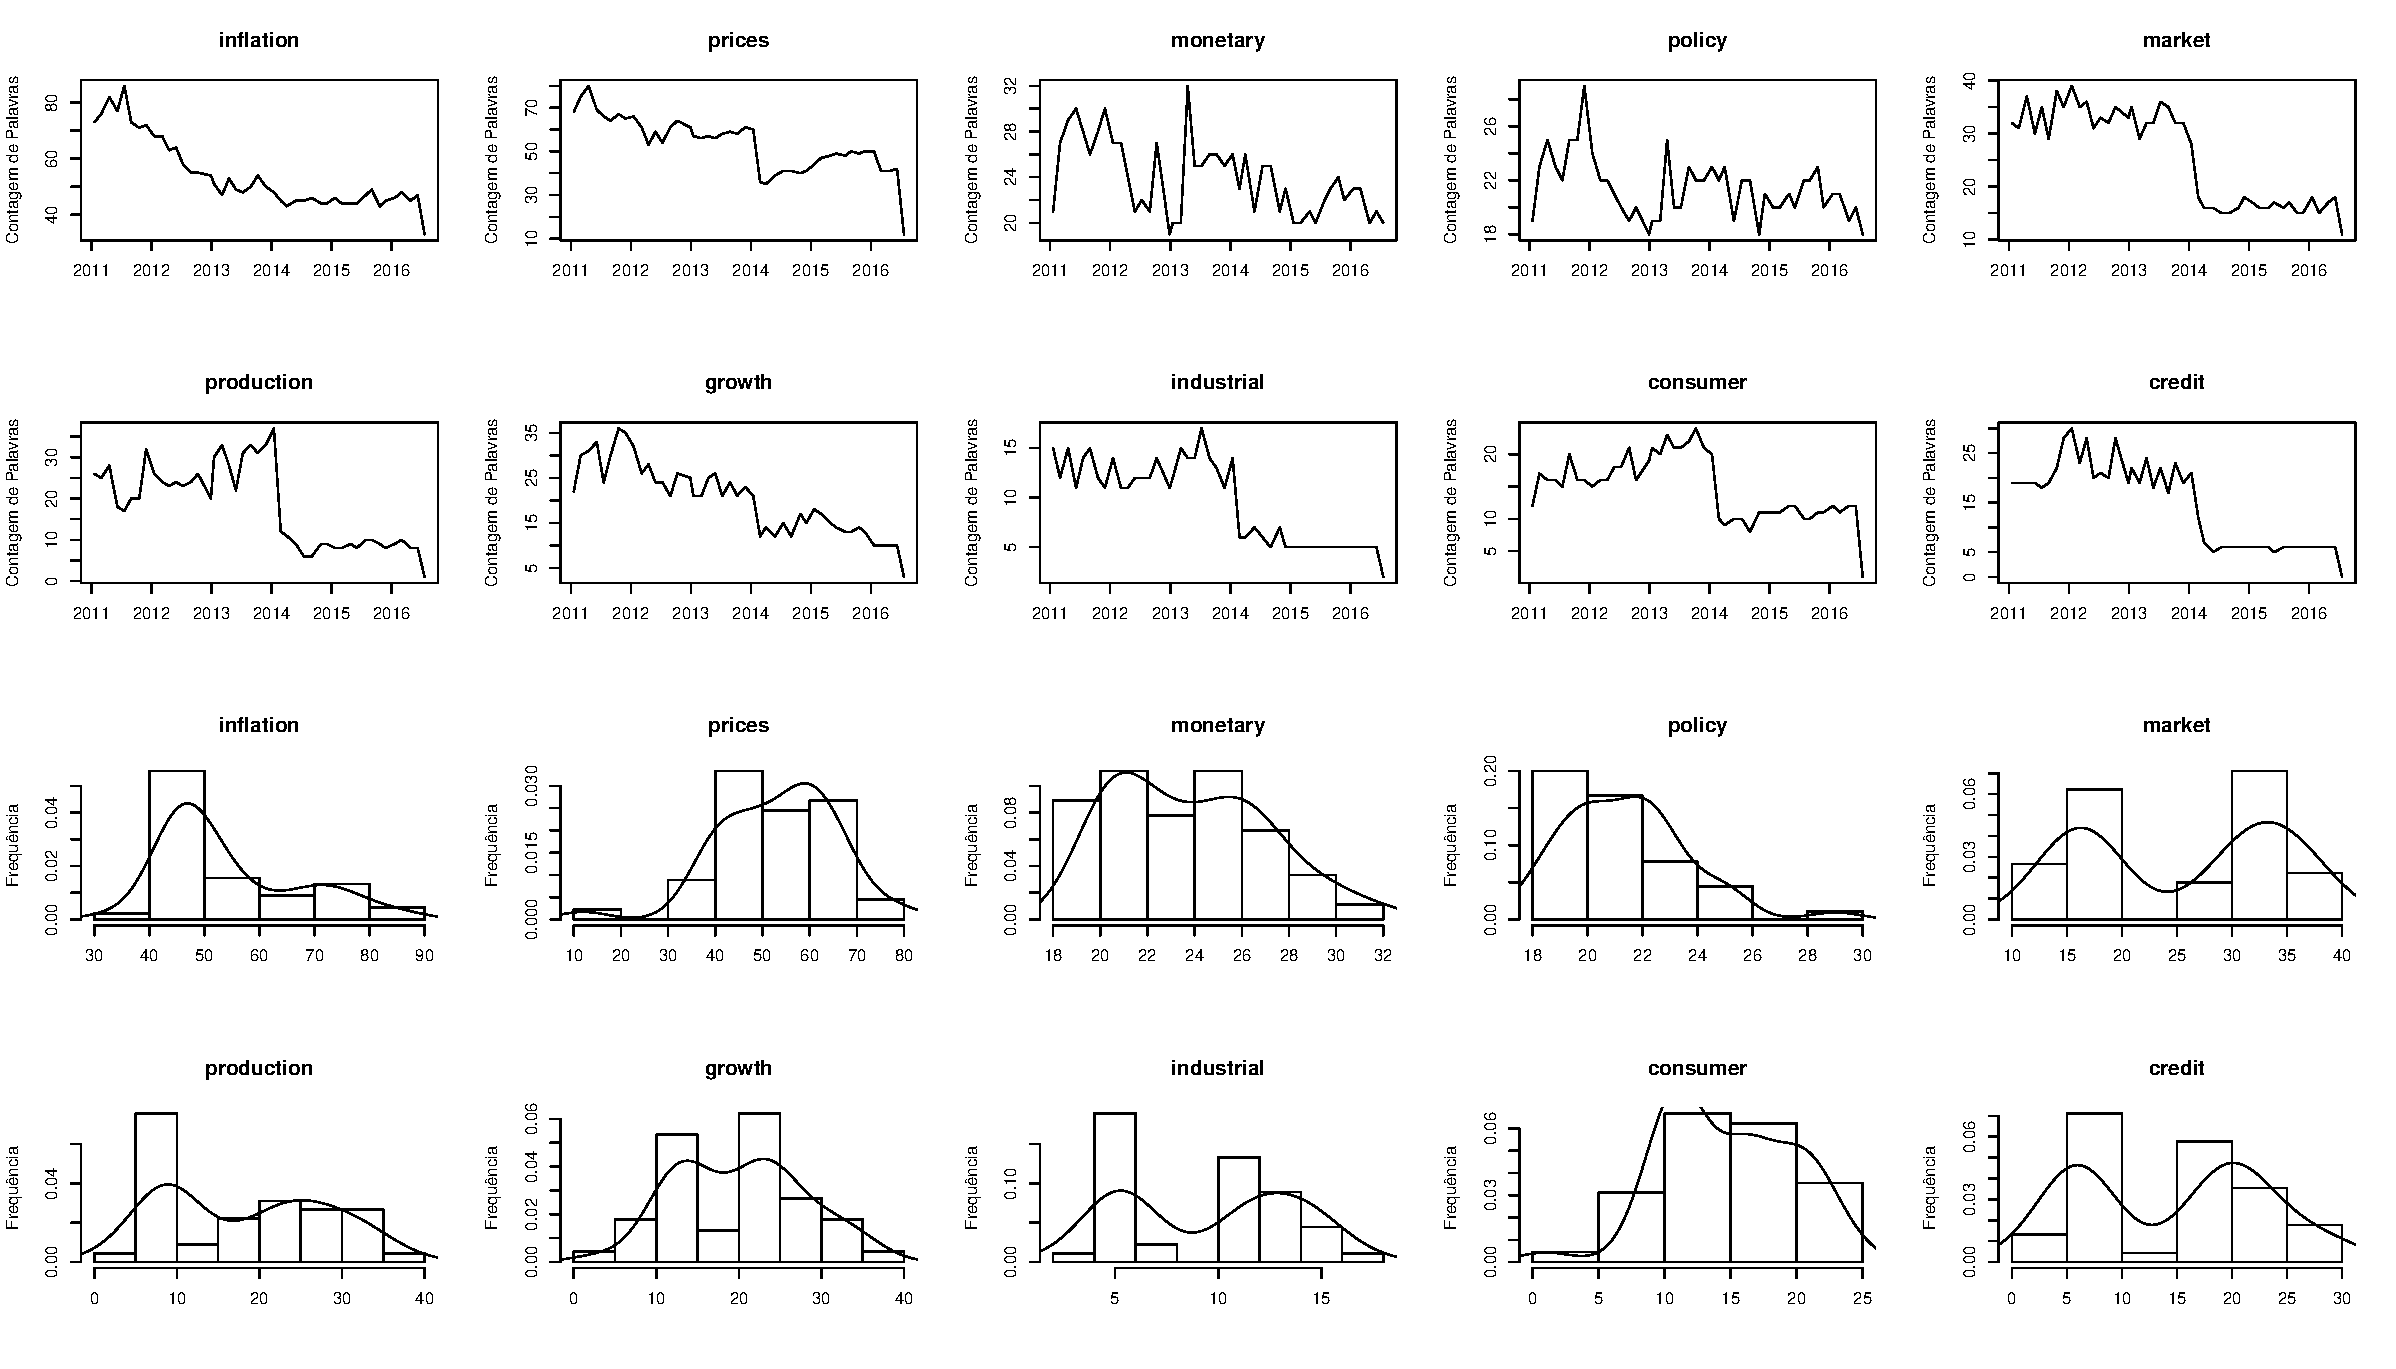
\includegraphics[width=1.5\textwidth]{capitulos/figures/analiseeconomicatombini.pdf}
    \caption{Frequência relativa das palavras de cunho econômico que mais aparecem (Gestão Tombini)}
    \label{fig:analiseeconomicatombini}
\end{figure}
\end{landscape}

\begin{landscape}
\begin{figure}
    \centering
    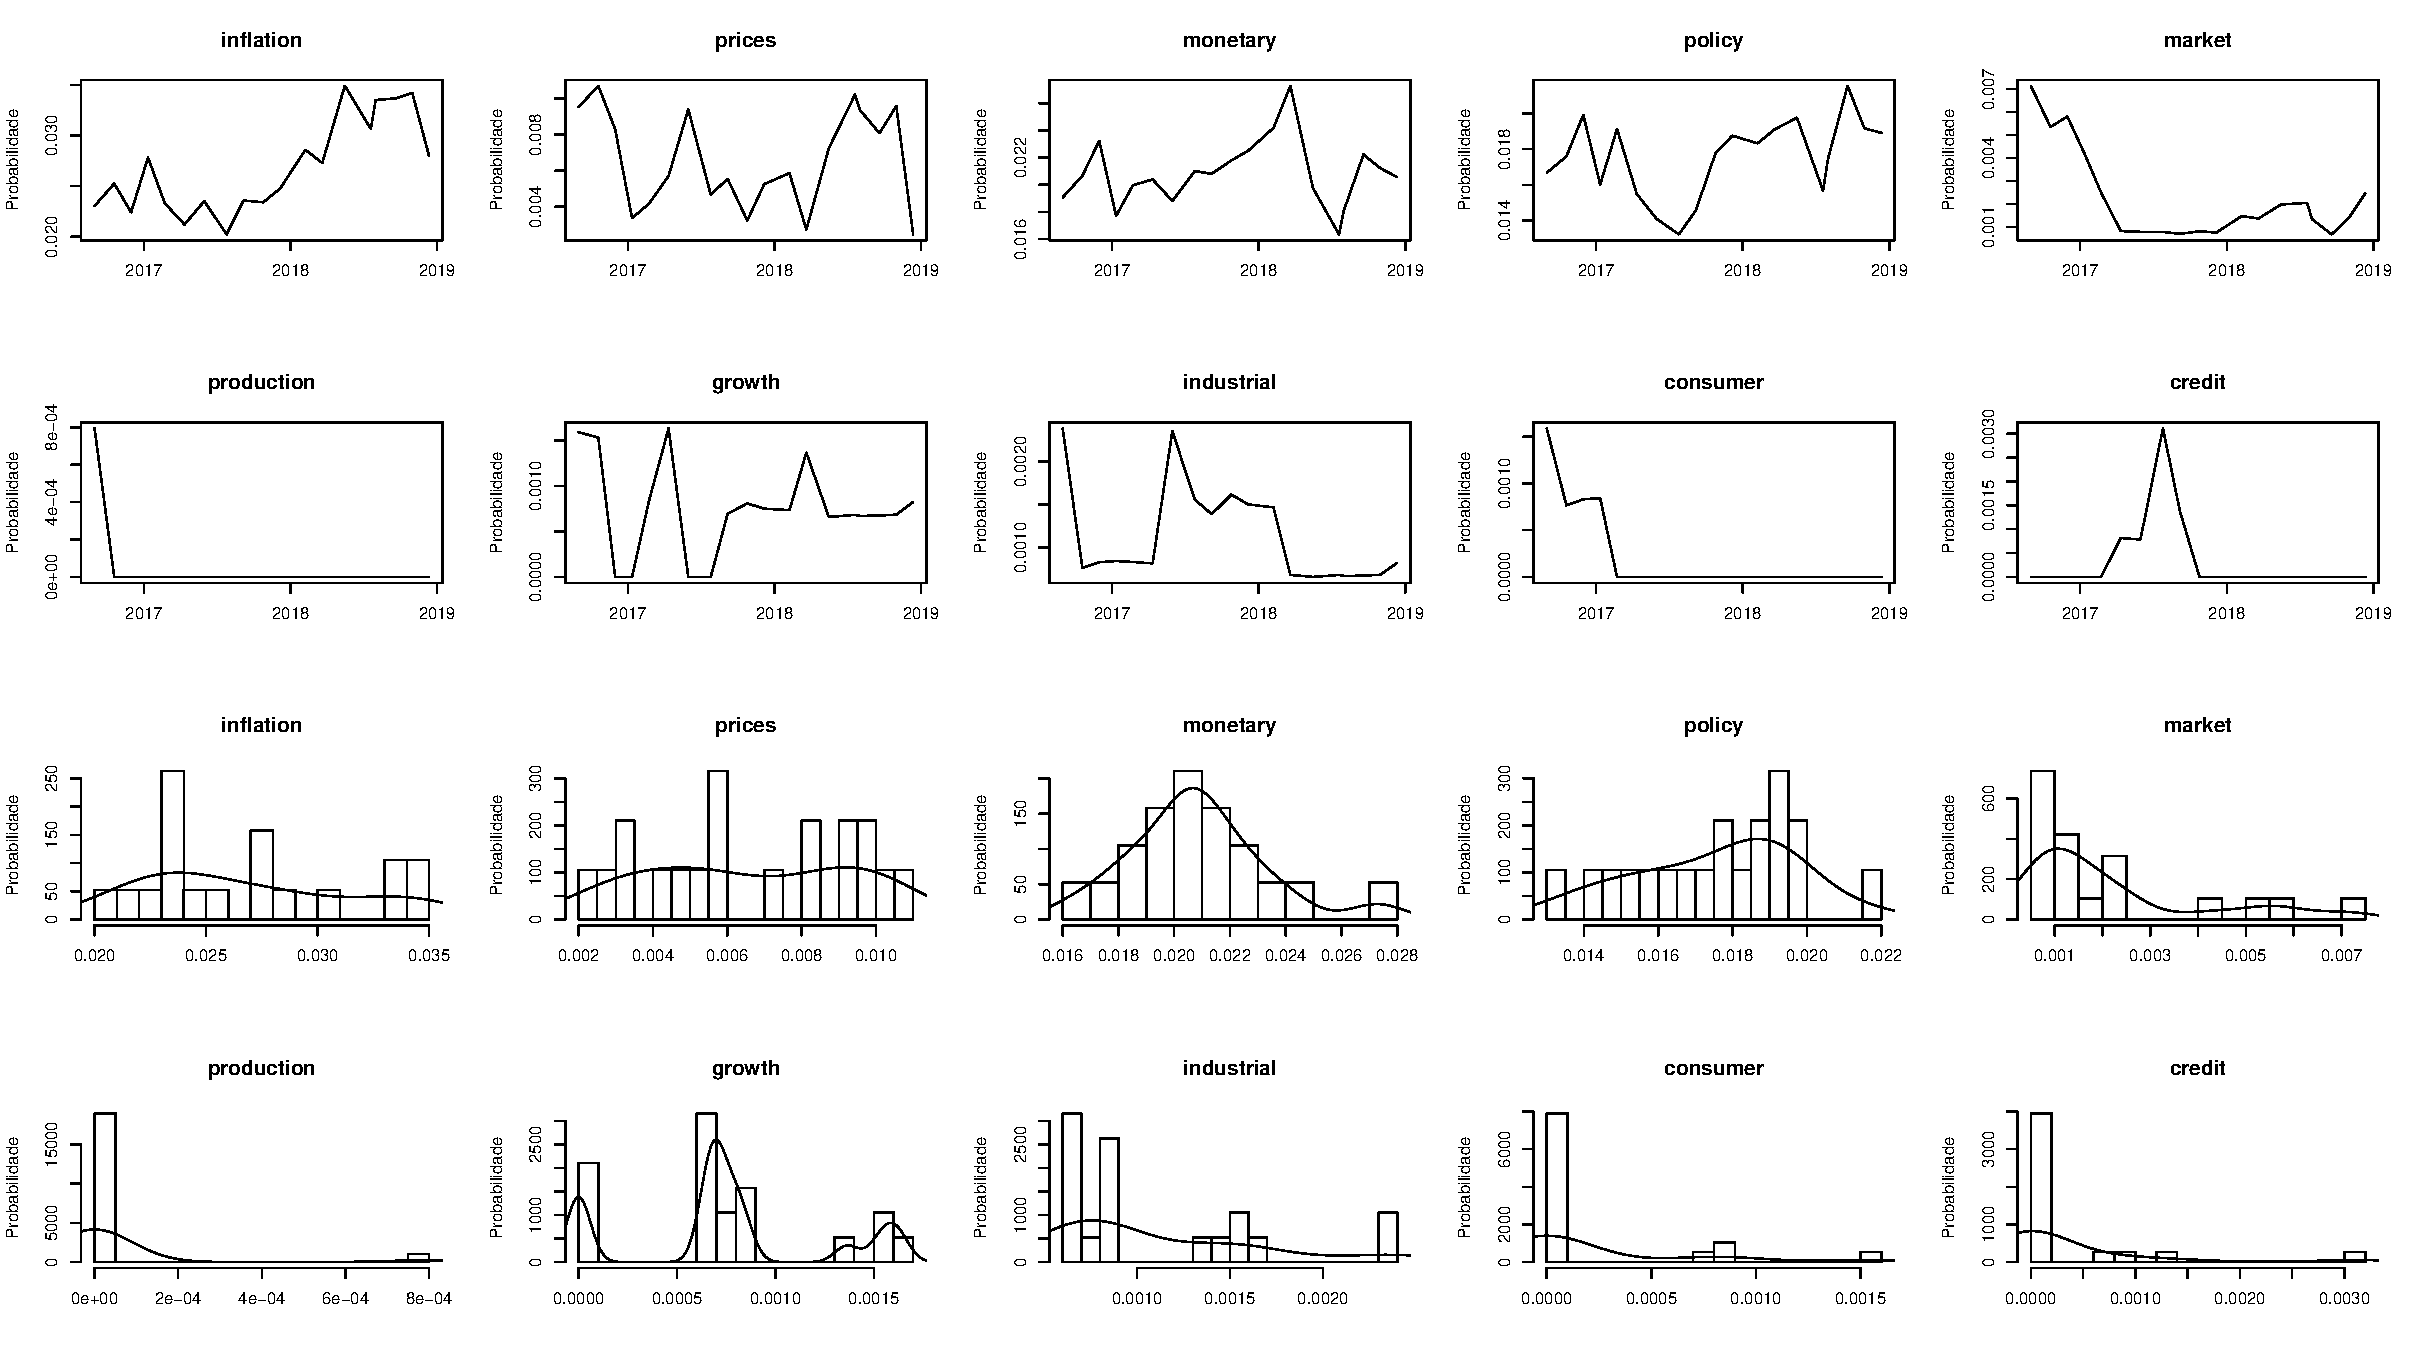
\includegraphics[width=1.5\textwidth]{capitulos/figures/analiserelativagoldfajn.pdf}
    \caption{Frequência relativa das palavras de cunho econômico que mais aparecem (Gestão Goldfajn)}
    \label{fig:analiserelativagoldfajn}
\end{figure}
\end{landscape}


%\end{apendicesenv}


\end{document}
